\chapter{用于快速采样的高阶求解器}\label{ch:solvers}


扩散模型的生成过程（将噪声映射到数据样本）可以通过反时 SDE 或其
相关的 PF-ODE。此过程本质上很慢，因为它依赖于通过许多小的积分步骤来近似解轨迹的数值求解器（有关简要介绍，请参阅 \Cref{app:de}）。因此，加速推理已成为一个中心研究目标。一般来说，现有的方法分为两类：
\begin{itemize}
    \item \textbfs{免训练方法：} 本章的重点。这些方法开发了先进的数值求解器，无需额外训练即可提高扩散采样的效率。
    \item \textbfs{ 基于训练的方法：} 在 \Cref{ch:distillation,ch:fast-scratch} 中进行了介绍。这些技术要么将预先训练的扩散模型蒸馏为快速生成器，要么直接学习 ODE 流映射（解决方案），以便只需要几个采样步骤。
\end{itemize}
基于 SDE 的采样器（例如，Euler--Maruyama）由于随机性可能会产生更多样的样本，但通常需要更多的步骤~\citep{xu2023restart}。在这里，我们关注基于 ODE 的生成，其原理自然延伸到 SDE 设置。

\chapterlearning{

  \item 将扩散采样视为 PF-ODE 的数值积分问题；

  \item 区分模型逼近误差和数值离散误差；

  \item 了解 DDIM、DEIS、DPM-Solver 和 DPM-Solver\texttt{++} 背后的主要数值思想；

  \item 将现代扩散采样器与经典数值方法连接起来，包括 Euler、Runge-Kutta (RK)、Adams-Bashforth (AB) 和指数积分器。

}{ 不熟悉微分方程或数值求解器的读者可以首先参考 \Cref{app:de}。在本章中，请记住一个问题：每个求解器精确积分什么，以及它在数值上近似什么？}


\clearpage


\section{序言}\label{sec:prologue-solvers}
\subsection{快速采样数值积分}

Score SDE 框架~\citep{song2020score} 建立了关键基础：
连接离散时间扩散模型和基于 ELBO 的公式
\citep{sohl2015deep,ho2020denoising} 具有连续时间 SDE/ODE
生成建模。这种联系提供了一种思考采样的清晰方法：
训练扩散模型后，生成可以被视为解决
学习了从噪声到数据的微分方程。

实际的困难是速度。一个天真的采样器遵循这个逆时
具有许多小数值步长的轨迹，通常需要数百或
数千次神经网络评估。快速采样询问我们是否可以
使用更少的模型调用来近似相同的生成过程。本章重点介绍 \emph{training-free} 加速：预训练
扩散模型保持固定，我们设计了更好的数值求解器
抽样。基于训练的加速方法，例如蒸馏或直接
几个步骤的训练，稍后会讨论
\Cref{ch:distillation,ch:fast-scratch}。

因此，本章的主要信息很简单：
\msgu{Message}{}{一旦训练了扩散模型，免训练快速采样在很大程度上是一个
数值积分问题.}

文献中包含许多命名的扩散采样器，它们可以使
主题看起来比实际情况更加支离破碎。在这一章中，我们首先
介绍这些方法背后的少量数值思想。
只有在之后我们才将熟悉的方法名称附加到它们上。这个
组织明确表示采样器并不是不相关的技巧：它们
是近似相同 PF-ODE 轨迹的不同方法。

\paragraph{采样求解经验PF-ODE.}
假设我们有一个预先训练的扩散模型
\[
    \rvs_{\bm{\phi}^\times}(\rvx,t)
    \approx
    \nabla_{\rvx}\log p_t(\rvx),
\]
或等效地用其他标准参数化之一编写的模型
来自 \Cref{sec:equivalent-parametrizations}。经验 PF-ODE 使用此
学习模型代替真实分数：
\[
    \frac{\diff \rvx(t)}{\diff t}
    =
    \rvf(\rvx(t),t)
    -
    \frac{1}{2}g^2(t)\,
    \rvs_{\bm{\phi}^\times}(\rvx(t),t).
\]
从$\rvx(T)\sim p_{\mathrm{prior}}$开始，一代集成了这个
ODE 从 $t=T$ 向后到 $t=0$。

对于两次$s>t$，精确的经验更新可以写成积分
形式为
\begin{align}
\label{eq:solution-int-score}
\begin{aligned}
    \widetilde\bPsi_{s\to t}(\rvx_s)
    =
    \rvx_s
    +
    \int_s^t
    \left[
        \rvf(\rvx(\tau),\tau)
        -
        \frac{1}{2}g^2(\tau)
        \rvs_{\bm{\phi}^\times}(\rvx(\tau),\tau)
    \right]\diff \tau .
\end{aligned}
\end{align}
这里，$\widetilde{\bPsi}_{s\to t}$ 表示经验的流映射
PF-ODE，通过将预言机分数替换为学习模型而获得。
在本书中，\emph{ 流映射} 指的是经典的 ODE
\Cref{eq:flow-map-def}中介绍的解决方案图。我们表示
相应的预言机流映射由$\bPsi_{s\to t}$提供。经验流
映射旨在近似预言机映射：
\[
    \widetilde{\bPsi}_{s\to t}(\rvx_s)
    \approx
    \bPsi_{s\to t}(\rvx_s).
\]
因为\Cref{eq:solution-int-score}中的积分不能通用
以封闭形式进行评估，数值采样器将
使用递减网格反转时间间隔
\begin{align}
\label{eq:time-step-def}
    T=t_0>t_1>\cdots>t_M=0,
\end{align}
开始于
\[
    \tilde{\rvx}_{t_0}=\rvx_T\sim p_{\mathrm{prior}},
\]
并产生一个序列
\[
    \tilde{\rvx}_{t_0},\tilde{\rvx}_{t_1},\ldots,\tilde{\rvx}_{t_M},
\]
其中 $\tilde{\rvx}_{t_i}$ 近似
$\widetilde\bPsi_{T\to t_i}(\rvx_T)$。最终迭代
$\tilde{\rvx}_{t_M}$用作生成的样本。

因此，本章中的每个免训练求解器都回答相同的问题：
\begin{question}
我们应该如何使用尽可能少的值准确地近似 PF-ODE 积分
模型评估是否可能？
\end{question}

\paragraph{求解器设计中的三种独立选择。}
一旦\Cref{eq:time-step-def}中的递减时间网格被引入，
区分经常交织在一起的三个选择是有用的
扩散采样。

\begin{enumerate}
    \item \textbfs{预测参数化.}
    预训练的扩散模型提供了哪些数量：
    分数 $\rvs_{\bm{\phi}^\times}$，噪音
    $\beps_{\bm{\phi}^\times}$，干净的数据
    $\rvx_{\bm{\phi}^\times}$，或速度
    $\rvv_{\bm{\phi}^\times}$？

    \item \textbfs{时间参数化。}
    哪个变量用于参数化沿着相同连续轨迹的进度？原始扩散时间 $t$ 是一种选择；其他重新参数化将在稍后有用时引入。

    \item \textbfs{数值近似。}
    求解器如何在有限区间内近似未知的模型相关量？它可以仅使用当前评估、在当前步骤中获取附加评估或重用先前步骤中的评估。
\end{enumerate}
这种分离在整章中都很重要。前两个选择确定呈现给求解器的数值形式，而第三个选择确定求解器如何使用可用的模型评估。




\paragraph{求解器如何使用模型评估？}
组织数值求解器的一种有用方法是询问下一次更新的信息来自哪里。从当前状态开始，求解器可以获取附加信息 \emph{在当前步骤内} 或重复使用来自 \emph{之前的步骤}.

A \emph{单步法} 仅使用当前状态和同一时间间隔内生成的评估来构造下一个状态。欧拉方法是最简单的示例，仅使用当前速度。高阶龙格-库塔 (RK) 方法可以在完成该步骤之前评估一个或多个中间状态的速度。因此，“单步”并不意味着“一个函数评估”；这意味着不需要先前完成的步骤中的信息。一个 \emph{多步法} 重用之前已完成步骤中的信息。存储的模型评估提供有关动态最近如何变化的信息，允许进行更高阶的更新，而无需在当前步骤中进行多次新的评估。 Adams--Bashforth（AB）家族是一个典型的典型例子。另一个想法是改变跨时间更新的安排方式。我们可以多次初始化状态并重复纠正它们，直到它们与 ODE 一致，而不是严格按顺序计算所有时间点。这种定点迭代可以允许在不同时间点并行进行模型评估。代表性的经典例子，包括欧拉、RK、AB 和皮卡德迭代，在
\Cref{app:de-solver-examples};它们的结构组织总结为
\Cref{eq:classic-solvers}.

\paragraph{计算成本和实际性能。}
数值时间步长不需要对应于单个神经网络评估。 Euler 每一步使用一次评估，而高阶 RK 方法可能需要多次评估。相反，多步方法会重用存储的评估，并且在初始化后，通常可以每一步仅使用一个新的评估来推进。因此，我们通过函数的 \emph{ 数量来衡量采样成本
评估} (NFE)。如果一种方法使用大约 $m$ 模型评估
跨过 $M$ 步骤，然后 
\[
\mathrm{NFE}\approx mM.
\]
例如，无分类器引导（参见 \Cref{sec:cfg}）需要
有条件和无条件模型预测，因此大约翻倍
每个采样步骤的神经网络评估成本。

这个经典的分类法告诉我们 \emph{ 数字信息来自哪里}
以及需要多少模型评估费用。扩散 PF-ODE 提供了额外的
机会：并非矢量场的每个部分都同样未知。取决于
在预测参数化上，确定了部分动态
通过噪声表进行分析，而仅剩余数量需要
神经网络评估。接下来我们研究如何暴露这种分离
改变 PF-ODE 的数值形式并激发特定扩散
积分器。






\subsection{扩散专用求解器的设计}
\label{subsec:common_design_solvers}

\Cref{app:de-solver} 中回顾的经典数值方法处理
通过评估其向量场来计算一般 ODE。扩散 PF-ODE 提供
附加结构：噪声表通过分析可知，而
扩散模型预测由神经网络提供。

这创造了一个有用的机会。而不是数值近似
以相同的方式处理动力学的每个部分，求解器可以保留已知的
依赖于时间表的项仅进行分析并近似
模型相关的预测。该结构暴露的清晰程度取决于
预测参数化。


\paragraph{I。超越分数的参数化。}
尽管 PF-ODE 可以写成分数形式，但现代实现通常
使用噪声预测、干净数据预测或速度预测。这些
参数化在代数上相关，但它们揭示了不同的数值
结构。还有一个重要的稳定性原因是避免直接分数预测
许多求解器。如$t\to 0$，真实分数
$\nabla_{\rvx}\log p_t(\cdot)$ 可以非常迅速地变化，特别是当
数据分布集中在低维流形附近
\citep{kim2022soft}。这使得训练有素的神经网络很难
直接近似分数以在小噪声水平附近保持准确~\footnote{要查看缩放比例，请回忆来自的预言机关系
\Cref{eq:predictions-equivalence}：
\[
    \beps^*(\rvx_t,t)
    =
    -\sigma_t\nabla_{\rvx}\log p_t(\rvx_t),
\]
其中$\beps^*(\rvx_t,t)
    =
    \mathbb{E}[\beps|\rvx_t]$是预言机噪声预测器，扰动核是$ \rvx_t|\rvx_0
    \sim
    \mathcal{N}(\rvx_t; \alpha_t\rvx_0,\sigma_t^2\rmI)$。由$L^2$中条件期望的正交性，
\[
    \mathbb{E}\|\beps\|_2^2
    =
    \mathbb{E}\|\beps^*\|_2^2
    +
    \mathbb{E}\|\beps-\beps^*\|_2^2,
\]
因此
\[
    \mathbb{E}\|\beps^*\|_2^2
    \le
    \mathbb{E}\|\beps\|_2^2
    =
    D,
\]
其中 $D$ 是数据维度。因此，预言机噪声预测器具有统一有界的期望平方范数。相比之下，oracle评分
\[
    \rvs^*(\rvx_t,t)
    :=
    \nabla_{\rvx}\log p_t(\rvx_t)
\]
满足
\[
    \mathbb{E}\|\rvs^*(\rvx_t,t)\|_2^2
    =
    \sigma_t^{-2}\,
    \mathbb{E}\|\beps^*(\rvx_t,t)\|_2^2
    \le
    \frac{D}{\sigma_t^2}.
\]
因此，直接分数预测可能会变得越来越糟糕，因为
$\sigma_t$ 变小，因为噪声预测转换为分数
通过因子 $1/\sigma_t$。这种缩放可以直接分数
在小噪声水平附近，数值参数化不太有利。}。


因此，一种广泛使用的替代方法是预测噪声
$\beps_{\bm{\phi}^\times}$，或相关目标，例如干净数据预测
或速度预测。在噪声预测形式中，分数近似为
\[
    \rvs_{\bm{\phi}^\times}(\rvx,t)
    =
    -\frac{1}{\sigma_t}\,
    \beps_{\bm{\phi}^\times}(\rvx,t).
\]
这些预测参数化在代数上是相关的，但是
神经网络提供的量只是求解器的一个组成部分
设计。接下来我们检查相同的 PF-ODE 如何在这些下以数字形式出现
不同的参数化。



\paragraph{II。一个 PF-ODE，两种数值形式.}
一旦选择了预测参数化，就可以使用相同的 PF-ODE
以两种特别有用的形式呈现给数值求解器。

\subparagraph{直速形式.}
最直接的体现就是
\begin{equation}
\label{eq:direct-pfode-form}
\frac{\diff \rvx(t)}{\diff t}
=
\rvv_{\bm{\phi}^\times}(\rvx(t),t).
\end{equation}
这里，在 $\rvv$ 预测下，模型直接提供完整的
经验 PF-ODE 速度 $\rvv_{\bm{\phi}^\times}(\rvx(t),t)$。数值
因此，积分方法将整个右侧离散为一个整体。\subparagraph{因子半线性形式.}
分数、噪声和干净数据预测自然会暴露额外的
依赖于时间表的结构。在每种情况下，PF-ODE 都可以写成
通用\emph{半线性}形式
\begin{equation}
\label{eq:general-semilinear-pfode}
\frac{\diff\rvx(t)}{\diff t}
=
\underbrace{
a(t)\rvx(t)
}_{\substack{\text{known}\\\text{linear part}}}
+
\underbrace{
b(t)
}_{\substack{\text{known}\\\text{coefficient}}}
\underbrace{
\rmN_{\bm{\phi}^\times}(\rvx(t),t)
}_{\substack{\text{neural}\\\text{evaluation}}},
\quad
\rmN_{\bm{\phi}^\times}
\in
\left\{
\rvs_{\bm{\phi}^\times},
\beps_{\bm{\phi}^\times},
\rvx_{\bm{\phi}^\times}
\right\}.
\end{equation}
这里，$a(t)$和$b(t)$是由噪声表确定的已知函数，
而 $\rmN_{\bm{\phi}^\times}$ 表示神经预测\footnote{In
标准半线性表示法，$b(t)\rmN_{\bm{\phi}^\times}$可吸收
转化为单个非线性项。我们将这两个因素分开，因为 $b(t)$
从噪声表中可以分析得知，而
$\rmN_{\bm{\phi}^\times}$ 需要神经网络评估。这允许
求解器近似积分内的神经预测，同时保留
并对已知的进度相关系数进行分析积分。}。术语
\emph{半线性}指的是这种分解：第一项是线性的
状态 $\rvx(t)$，而神经项可能非线性地依赖于 $\rvx(t)$。
这种分离并不唯一，但在数值上特别有用，因为
已知的线性部分通常可以进行分析处理，只留下神经网络
贡献以数字形式近似。

对于三个标准半线性参数化\footnote{如下
部分，我们在 SDE 系数 $(f(t),g(t))$ 和高斯系数之间切换
扰动核 $\rvx_t | \rvx_0
    \sim
    \mathcal{N}
    \bigl(
        \rvx_t;
        \alpha_t\rvx_0,
        \sigma_t^2\rmI
    \bigr)$。
它们的关系是
\[
    f(t)
    =
    \frac{\alpha_t'}{\alpha_t},
    \qquad
    g^2(t)
    =
    \frac{\diff}{\diff t}\bigl(\sigma_t^2\bigr)
    -
    2\frac{\alpha_t'}{\alpha_t}\sigma_t^2
    =
    2\sigma_t\sigma_t'
    -
    2\frac{\alpha_t'}{\alpha_t}\sigma_t^2.
\]
}，$a(t)$、$b(t)$的对应选择，以及
$\rmN_{\bm{\phi}^\times}$ 列在 \Cref{tb:pf-ode-parameterizations} 中。例如，在噪声预测下，
\begin{equation}
\label{eq:noise_pf_ode}
\frac{\diff\rvx(t)}{\diff t}
=
\underbrace{
f(t)\rvx(t)
}_{\text{linear part}}
+
\underbrace{
\frac{1}{2}\frac{g^2(t)}{\sigma_t}
\beps_{\bm{\phi}^\times}(\rvx(t),t)
}_{\text{nonlinear neural part}}.
\end{equation}
乘以神经预测的系数完全可以从
噪音时间表；第二项中唯一学到的量是
$\beps_{\bm{\phi}^\times}(\rvx(t),t)$。

\begin{table}[th!]
\caption{ 用于分数、噪声和干净数据预测的因子 PF-ODE 形式。}
\small
\centering
\renewcommand{\arraystretch}{1.35}
\begin{tabularx}{0.88\linewidth}{
    @{}
    >{\raggedright\arraybackslash}p{0.20\linewidth}
    >{\centering\arraybackslash}p{0.19\linewidth}
    >{\centering\arraybackslash}X
    >{\centering\arraybackslash}p{0.22\linewidth}
    @{}
}
\toprule
\textbfs{预测} &
$\boldsymbol{a(t)}$ &
$\boldsymbol{b(t)}$ &
$\boldsymbol{\rmN_{\bm{\phi}^\times}}$ \\
\midrule

$\rvs$-预测&
$f(t)$ &
$-\frac{1}{2}g^2(t)$ &
$\rvs_{\bm{\phi}^\times}$ \\

\graymidrule

$\beps$-预测&
$f(t)$ &
$\displaystyle \tfrac{1}{2}\tfrac{g^2(t)}{\sigma_t}$ &
$\beps_{\bm{\phi}^\times}$ \\

\graymidrule

$\rvx$-预测&
$\displaystyle \tfrac{\sigma_t'}{\sigma_t}$ &
$\displaystyle
\alpha_t
\left(
\tfrac{\alpha_t'}{\alpha_t}
-
\tfrac{\sigma_t'}{\sigma_t}
\right)$ &
$\rvx_{\bm{\phi}^\times}$ \\

\bottomrule
\end{tabularx}
\label{tb:pf-ode-parameterizations}
\end{table}

在预言机级别，分数、噪声、干净数据和速度预测是同一 PF-ODE 的完全相同的表示。对于经验模型，当通过同一模型输出的精确代数转换获得不同的预测参数化时，相同的等价性成立（参见
\Cref{eq:predictions-equivalence}）。在这种情况下，相同的经验 PF-ODE 可以通过分数、噪声、干净数据或速度预测来表达。得到的公式看起来不同，因为它们暴露了不同的数值结构，但它们描述了相同的学习连续动态。然而，如果针对不同的预测目标独立训练单独的网络，则它们的经验 PF-ODE 不需要完全一致。在这种情况下，采样器之间的差异可能反映模型近似和数值离散。
\paragraph{三．半线性 PF-ODE 的指数积分器。}
因式分解的半线性形式 \Cref{eq:general-semilinear-pfode} 将分析已知的线性动力学与模型相关的预测分开。对于 $s>t$，定义积分因子
\[
\mathcal{E}(s\shortrightarrow t)
:=
\exp\left(
\int_s^t a(u)\diff u
\right).
\]
常数变分公式给出精确的经验 PF-ODE 流
\begin{mdframed}
\begin{equation}
\label{eq:factored-variation-of-constants}
\widetilde\bPsi_{s\to t}(\rvx_s)
=
\mathcal{E}(s\shortrightarrow t)\rvx_s
+
\int_s^t
\mathcal{E}(\tau\shortrightarrow t)
b(\tau)
\rmN_{\bm{\phi}^\times}(\rvx_\tau,\tau)
\diff\tau .
\end{equation}
\end{mdframed}
我们建议读者参考 \Cref{app:exp-int-factor} 用于一般推导。例如，在噪声预测下，
$a(t)=f(t)$,
$b(t)=\tfrac{1}{2}g^2(t)/\sigma_t$, 和
$\rmN_{\bm{\phi}^\times}=\beps_{\bm{\phi}^\times}$，所以
\begin{equation}
\label{eq:variation_of_constants}
\widetilde\bPsi_{s\to t}(\rvx_s)
=
\underbrace{
\mathcal{E}(s\shortrightarrow t)\rvx_s
}_{\text{exact linear evolution}}
+
\frac{1}{2}
\int_s^t
\frac{g^2(\tau)}{\sigma_\tau}
\mathcal{E}(\tau\shortrightarrow t)
\beps_{\bm{\phi}^\times}(\rvx_\tau,\tau)
\diff\tau,
\end{equation}
其中
$\mathcal{E}(s\shortrightarrow t)
=
\exp\!\left(\int_s^t f(u)\diff u\right)$。现在，数字机会已经很明显了。积分因子和系数 $b(\tau)$ 由扩散时间表确定；积分内唯一的未知量是沿轨迹评估的神经预测。因此，保持这些已知因素的明确性允许一阶近似仅作用于神经预测，而不是吸收系数加权乘积
$b(\tau)\rmN_{\bm{\phi}^\times}(\rvx_\tau,\tau)$ 转化为单个未知残差。

\paragraph{为什么因式分解指数积分器形式有帮助。}
要了解这种分离的好处，请将其与从精确经验 PF-ODE 状态向后一步的普通欧拉进行比较 $\rvx_s$ 当时 $s$ 至
$t<s$。定义 $\Delta s:=s-t>0$ 和
$\rmN_s:=\rmN_{\bm{\phi}^\times}(\rvx_s,s)$.Plain Euler 将完整的 PF-ODE 速度视为局部常数，
$a(\tau)\rvx_\tau+
b(\tau)\rmN_{\bm{\phi}^\times}(\rvx_\tau,\tau)
\approx a(s)\rvx_s+b(s)\rmN_s$ 为 $\tau\in[t,s]$，给出
\begin{align}
\label{eq:euler-step}
\tilde\rvx_t^{\mathrm{Euler}}
=
\rvx_s
-
\Delta s
\left[
a(s)\rvx_s+b(s)\rmN_s
\right].
\end{align}
相反，我们可以只固定神经预测，
$\rmN_{\bm{\phi}^\times}(\rvx_\tau,\tau)\approx\rmN_s$，同时保留
已知的时间表依赖性
\Cref{eq:factored-variation-of-constants}。这给出了
\emph{一阶因式分解指数积分器更新}\footnote{更新
\Cref{eq:factored-ei-step} 中的原始状态和时间不是普通欧拉
变量。在对状态进行积分因子变换之后，每隔一段时间
其中生成的时间坐标是单调的，相应的时间
重新参数化，它可以写成普通的显式欧拉步骤。我们使这种连接具体化以利于扩散
DDIM部分采样。}
\begin{align}
\label{eq:factored-ei-step}
\tilde\rvx_t^{\mathrm{EI}}
=
\mathcal E(s\shortrightarrow t)\rvx_s
+
\left[
\int_s^t
\mathcal E(\tau\shortrightarrow t)b(\tau)\diff\tau
\right]\rmN_s.
\end{align}
两种方法每一步都使用一次神经网络评估。普通欧拉冻结
完整的 PF-ODE 速度，而因子更新保持已知
时间表依赖性并仅冻结神经预测。这个因式分解
重要事项：如果
$b(\tau)\rmN_{\bm{\phi}^\times}(\rvx_\tau,\tau)$
相反，被视为单个残差并保持固定，结果是
传统指数欧拉。因此，因子更新又保留了一项
已知量，$b(\tau)$，在积分内；两个更新同时发生
$b(\tau)$ 在步长上保持恒定。

一个简单的冻结预测示例使这种差异变得具体。假设
$a(t)\equiv a$、$b(t)\equiv b$ 和
$\rmN_{\bm{\phi}^\times}(\rvx_\tau,\tau)\equiv\rmN_s$ 越过台阶。对于
$a\neq0$，
\begin{align*}
\tilde\rvx_t^{\mathrm{EI}}
&=
e^{-a\Delta s}\rvx_s
+
\frac{b}{a}
\left(
e^{-a\Delta s}-1
\right)\rmN_s,
\\
\tilde\rvx_t^{\mathrm{Euler}}
&=
(1-a\Delta s)\rvx_s
-
b\Delta s\,\rmN_s.
\end{align*}
扩展分解更新给出
\begin{align*}
\tilde\rvx_t^{\mathrm{EI}}
=
\tilde\rvx_t^{\mathrm{Euler}}
+
\frac{(\Delta s)^2}{2}
\left[
a^2\rvx_s
+
ab\,\rmN_s
\right]
+
\mathcal O((\Delta s)^3).
\end{align*}
因此，这两个更新同意小步骤的第一顺序，而分解后的
更新保留了已知动态的高阶效应。区别
对于更大的步骤来说可能变得很重要。例如，当 $a>0$ 时，确切的
乘数 $e^{-a\Delta s}$ 保持正值且收缩
$\Delta s>0$，而欧拉近似 $1-a\Delta s$ 变为负数
当 $a\Delta s>1$ 时，并且当 $a\Delta s>2$ 时幅度大于 1。
因此，普通欧拉可能会扭曲分解形式已经存在的动力学
进行分析处理。

在完整的 PF-ODE 中，神经预测通常沿着
轨迹。从精确值中减去 \Cref{eq:factored-ei-step}
常数变分公式给出
\begin{align}
\label{eq:ei-local-defect}
\widetilde\bPsi_{s\to t}(\rvx_s)
-
\tilde\rvx_t^{\mathrm{EI}}
=
\int_s^t
\mathcal E(\tau\shortrightarrow t)b(\tau)
\Big[
\rmN_{\bm{\phi}^\times}(\rvx_\tau,\tau)
-
\rmN_s
\Big]\diff\tau.
\end{align}
因此，一旦对已知的与时间表相关的动态进行分析处理，
剩余的离散化误差由神经网络的变化控制
沿着轨迹进行预测。这种分离是基本的数值
几个特定于扩散的求解器将在不同的情况下利用的原理
方式。\subsection{从数值思想到扩散采样器的路线图}
本章的其余部分将展示这些数字概念如何在现代中出现
扩散采样器。我们从 \Cref{sec:revisit-ddim} 中的 DDIM 开始，其中
根据当前模型预测构造一阶更新。然后我们研究
\Cref{sec:exponential} 中的 DEIS，它使用之前步骤的预测来
建立高阶近似。 \Cref{sec:dpm} 中的 DPM-Solver 开发
使用当前的额外模型评估进行高阶更新
步骤。 DPM-Solver\texttt{++}在\Cref{sec:dpm++}中开发了两个对应的
基于干净数据预测的变体：单步变体，
DPM-Solver\texttt{++}(2S)，它使用当前的附加评估
步骤，以及多步骤变体 DPM-Solver\texttt{++}(2M)，它重用
之前步骤的预测。最后，\Cref{sec:picard}介绍
ParaDiGMS，通过定点一起更新几个时间点
迭代以实现跨时间的并行计算。

下表提供了将这些扩散采样器与
\Cref{eq:classic-solvers} 中回顾了经典的数值思想。

\begin{center}
\small
\renewcommand{\arraystretch}{1.25}
\begin{tabularx}{0.98\linewidth}{
    @{}
    >{\raggedright\arraybackslash}p{0.21\linewidth}
    >{\raggedright\arraybackslash}p{0.32\linewidth}
    >{\raggedright\arraybackslash}X
    >{\raggedright\arraybackslash}p{0.13\linewidth}
    @{}
}
\toprule
\textbfs{经典理念} &
\textbfs{更新是如何构建的} &
\textbfs{扩散示例} &
\textbfs{其中} \\
\midrule

欧拉型一阶更新 &
使用该步骤开始时的模型预测前进到下一步
状态。 &
DDIM； DPM-Solver-1 &
\Cref{sec:revisit-ddim,sec:dpm} \\

\graymidrule

RK型分阶段更新&
在完成之前在其他中间状态评估模型
当前步骤。 &
高阶 DPM-Solver； DPM-Solver\texttt{++}(2S) &
\Cref{sec:dpm,sec:dpm++} \\

\graymidrule

AB型多步更新 &
重用先前步骤中的模型预测来构建下一个更新。 &
DEIS； DPM-Solver\texttt{++}(2M) &
\Cref{sec:exponential,sec:dpm++} \\

\graymidrule

Picard型定点迭代 &
一起更新几个时间点并反复细化它们的状态。 &
ParaDiGMS &
\Cref{sec:picard} \\

\bottomrule
\end{tabularx}
\end{center}

这些联系为这些方法提供了高级数字路线图
下面展开。扩散求解器进一步受益于特定的结构
PF-ODE，包括不同的预测参数化，分析已知
与时间表相关的系数和替代时间参数化。

为了保持演示的系统性，每个部分都遵循相同的大致结构：我们首先推导扩散求解器并解释它所利用的数值思想，然后将其与相应的经典求解器原理联系起来，最后将其与本章中开发的其他扩散求解器联系起来。该组织明确了共同的数字主干和区分所得方法的特定扩散成分。





\clearpage
\newpage

\section{\texorpdfstring{DDIM}{DDIM}}\label{sec:revisit-ddim}

\emph{去噪扩散隐式模型} （DDIM）~\citep{song2020denoising}
是最早、应用最广泛的加速扩散采样方法之一。尽管 DDIM 最初是从概率角度引入的，但其确定性更新也允许通过 PF-ODE 进行特别清晰的解释。因此，我们在本章的通用数值 ODE 求解框架下引入 DDIM，并将其原始变分视角推迟到 \Cref{subsec:ddim}。序言在 \Cref{sec:prologue-solvers} 给我们留下了一个具体的数值问题：一旦通过分析保留了已知的与时间表相关的因素，我们应该如何近似剩余积分内的神经预测？ DDIM 采用最简单的答案： \emph{在步骤开始时使用其值}。我们首先推导所得更新，然后阐明其与经典欧拉积分以及稍后介绍的高阶扩散求解器的关系。


\subsection{DDIM 作为一阶扩散求解器}\label{subsec:ddim-different-para}

考虑从起点开始的一个采样步骤\footnote{在本章中， $\tilde{\rvx}_s$ 表示时间级别的状态 $s$ 用于初始化当前求解器步骤，通常从先前的数值步骤获得。波形符将其与 $\rvx_s$，表示来自精确扩散分布的预言样本，或者 $\rvx_s \sim p_s$ 或者，条件为 $\rvx_0$, $\rvx_s \sim p_s(\,\cdot \mid \rvx_0)$。因此， $\tilde{\rvx}_s$ 不需要根据 $p_s$.} $\tilde\rvx_s$ 当时 $s$ 至 $t<s$。在噪声预测下，
\Cref{eq:variation_of_constants} 给出精确的经验 PF-ODE 流
\begin{align*}
\widetilde\bPsi_{s\to t}(\tilde\rvx_s)
=
\mathcal E(s\shortrightarrow t)\tilde\rvx_s
+
\frac{1}{2}
\int_s^t
\frac{g^2(\tau)}{\sigma_\tau}
\mathcal E(\tau\shortrightarrow t)
\beps_{\bm{\phi}^\times}(\rvx_\tau,\tau)
\diff\tau .
\end{align*}
通过分析可知与进度相关的因素；积分中唯一未知的量是神经预测
$\beps_{\bm{\phi}^\times}(\rvx_\tau,\tau)$ 沿着未知轨迹评估。从 PF-ODE 的角度来看，确定性 DDIM 使用最简单的一阶近似：它将噪声预测固定在步骤开始时的值，
\[
\beps_{\bm{\phi}^\times}(\rvx_\tau,\tau)
\approx
\beps_{\bm{\phi}^\times}(\tilde\rvx_s,s),\quad\text{for}\quad \tau\in[t,s],
\]
 同时保留积分内已知的与计划相关的因素。这给出了
\begin{align*}
\tilde\rvx_t
=
\mathcal E(s\shortrightarrow t)\tilde\rvx_s
+
\left[
\frac{1}{2}
\int_s^t
\frac{g^2(\tau)}{\sigma_\tau}
\mathcal E(\tau\shortrightarrow t)
\diff\tau
\right]
\beps_{\bm{\phi}^\times}(\tilde\rvx_s,s).
\end{align*}

使用 $f(t)=\alpha_t'/\alpha_t$，积分因子简化为
$\mathcal E(s\shortrightarrow t)=\alpha_t/\alpha_s$。剩余的与计划相关的系数也有一个方便的封闭形式：
$\tfrac{1}{2}\tfrac{g^2(\tau)}{\sigma_\tau}
\mathcal E(\tau\shortrightarrow t)
=
\alpha_t
\tfrac{\diff}{\diff\tau}
\bigl(\tfrac{\sigma_\tau}{\alpha_\tau}\bigr)$。因此，一旦神经预测在该步骤中保持固定，就可以根据噪声表准确地评估剩余积分。

\proppp{DDIM 作为一阶因子 EI 更新}{ddim-euler}{
对于 $s>t$，确定性 DDIM 给出
\begin{align}
\label{eq:ddim-euler}
\tilde\rvx_t
=
\frac{\alpha_t}{\alpha_s}\tilde\rvx_s
+
\alpha_t
\left(
\frac{\sigma_t}{\alpha_t}
-
\frac{\sigma_s}{\alpha_s}
\right)
\beps_{\bm{\phi}^\times}(\tilde\rvx_s,s).
\end{align}
}{
积分得出结果
$\frac{\diff}{\diff\tau}(\sigma_\tau/\alpha_\tau)$
来自 $s$ 至 $t$.
}

因此，DDIM 所做的近似非常具体：在整个时间间隔内保留已知的时间表演化，而仅忽略神经预测的变化。在干净数据预测下有类似的推导。精确的经验 PF-ODE 流可以写为
\begin{align*}
\widetilde\bPsi_{s\to t}(\tilde\rvx_s)
=
\frac{\sigma_t}{\sigma_s}\tilde\rvx_s
+
\sigma_t
\int_s^t
\frac{\diff}{\diff\tau}
\left(
\frac{\alpha_\tau}{\sigma_\tau}
\right)
\rvx_{\bm{\phi}^\times}(\rvx_\tau,\tau)
\diff\tau.
\end{align*}
使用与上面相同的一阶近似，我们认为
$\rvx_{\bm{\phi}^\times}(\rvx_\tau,\tau)$ 固定为当时的值 $s$。然后精确评估剩余的与计划相关的积分，给出
\[
\tilde\rvx_t
=
\frac{\sigma_t}{\sigma_s}\tilde\rvx_s
+
\alpha_s
\left(
\frac{\alpha_t}{\alpha_s}
-
\frac{\sigma_t}{\sigma_s}
\right)
\rvx_{\bm{\phi}^\times}(\tilde\rvx_s,s).
\]
因此，冻结噪声预测 PF-ODE 中的噪声预测或冻结干净数据 PF-ODE 中的干净数据预测会产生相同的 DDIM 更新。此对应关系稍后将再次出现在 DPM-Solver 和 DPM-Solver 中\texttt{++}，分别根据噪声和干净数据预测公式构建高阶近似。

\paragraph{等效形式和解释。}
在预言机级别，标准预测目标通过以下方式在点代数上等效 \Cref{eq:predictions-equivalence}。因此，上面从噪声预测导出的确定性DDIM更新可以在起点重写 $s$ 在干净数据或分数预测方面，不改变有限步更新。以下推论收集了这些等价表达式。

\cornp{确定性 DDIM 更新的等效形式}{
让 $s>t$，并考虑一个状态 $\tilde\rvx_s$ 当时 $s$。 oracle 确定性 DDIM 更新接受等效表达式
\begin{align}
\begin{aligned}
\label{eq:ddim-update-all}
\tilde\rvx_t
&=
\frac{\alpha_t}{\alpha_s}\tilde\rvx_s
+
\alpha_t
\left(
\frac{\sigma_t}{\alpha_t}
-
\frac{\sigma_s}{\alpha_s}
\right)
\beps^*(\tilde\rvx_s,s)
\\
&=
\frac{\sigma_t}{\sigma_s}\tilde\rvx_s
+
\alpha_s
\left(
\frac{\alpha_t}{\alpha_s}
-
\frac{\sigma_t}{\sigma_s}
\right)
\rvx^*(\tilde\rvx_s,s)
\\
&=
\frac{\alpha_t}{\alpha_s}\tilde\rvx_s
+
\sigma_s^2
\left(
\frac{\alpha_t}{\alpha_s}
-
\frac{\sigma_t}{\sigma_s}
\right)
\rvs^*(\tilde\rvx_s,s)
\\
&=
\alpha_t
\underset{\substack{
\approx\rvx_{\bm{\phi}^\times}\\
\text{estimated clean}
}}{
\underbrace{\rvx^*(\tilde\rvx_s,s)}
}
+
\sigma_t
\underset{\substack{
\approx\beps_{\bm{\phi}^\times}\\
\text{estimated noise}
}}{
\underbrace{\beps^*(\tilde\rvx_s,s)}
}.
\end{aligned}
\end{align}
}

最后一个恒等式 \Cref{eq:ddim-update-all} 给出了 DDIM 特别直观的视图。开始于 $\tilde\rvx_s$，DDIM 保持及时推断的干净和噪声估计 $s$ 使用目标调度系数修复并重新组合它们：
\[
\tilde\rvx_t
=
\alpha_t\rvx^*(\tilde\rvx_s,s)
+
\sigma_t\beps^*(\tilde\rvx_s,s).
\]
这反映了前向高斯路径的共享噪声耦合，
$\rvx_\tau=\alpha_\tau\rvx_0+\sigma_\tau\beps$: 以固定对为条件
$(\rvx_0,\beps)$，从一个时间移动到另一个时间仅更改系数
$(\alpha_\tau,\sigma_\tau)$。 DDIM 使用步骤开始时可用的干净和噪声估计来应用相同的想法。在条件层面上，其中 $\rvx_0$ 和 $\beps$ 是固定的，这种重组完全遵循相应的共享噪声路径。然而，在边缘水平上， $\rvx^*(\tilde\rvx_s,s)$ 和
$\beps^*(\tilde\rvx_s,s)$ 后验估计是从
$\tilde\rvx_s$。因此，有限 DDIM 步骤通常是边缘 PF-ODE 流的近似值，而不是从 $p_t$.\begin{figure}[th!]
    \centering
    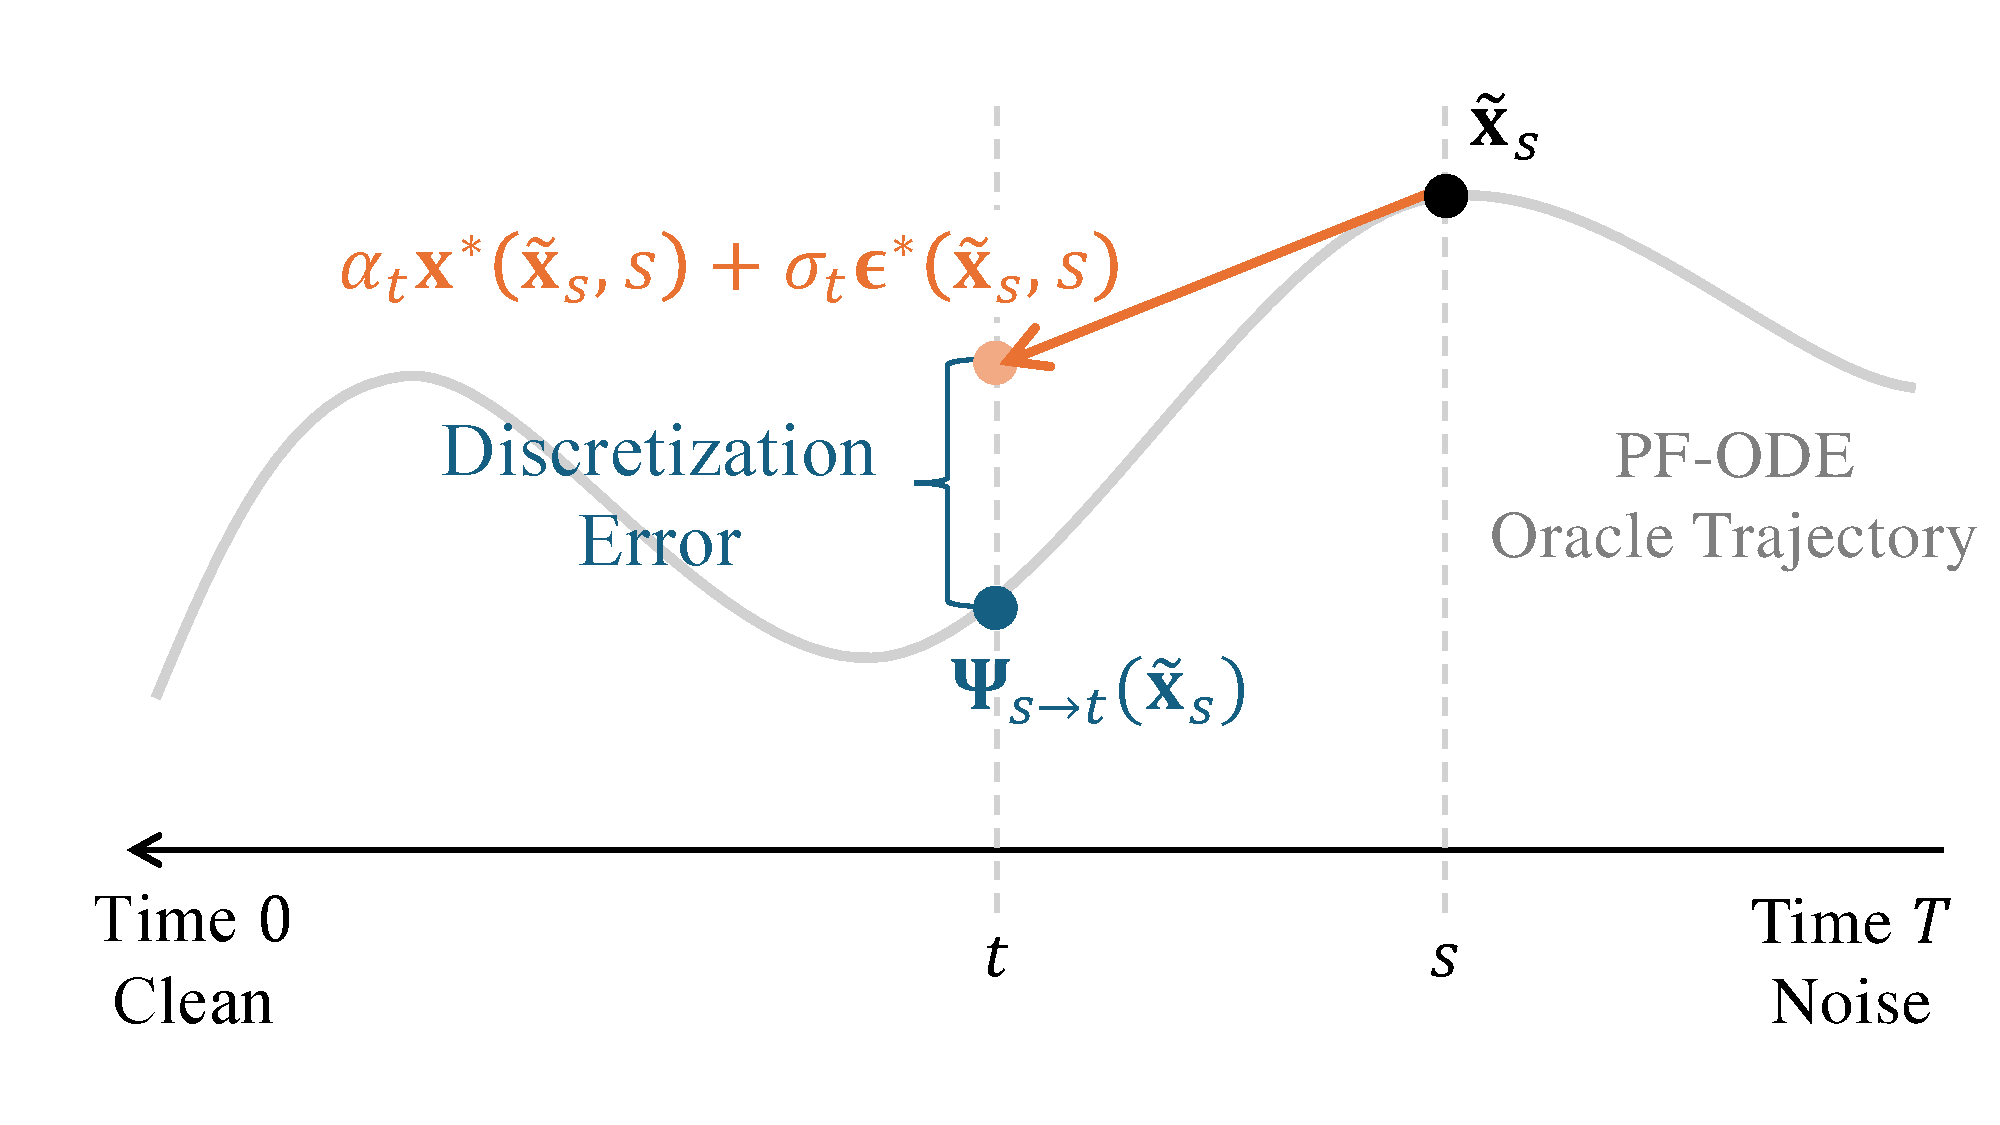
\includegraphics[width=0.86\linewidth]{Images/PartB/Euler.pdf}
    \caption{\textbfs{有限步 DDIM 与经验 PF-ODE 流。}
    从$\tilde\rvx_s$开始，经验PF-ODE不断演化
    为 $\widetilde\bPsi_{s\to t}(\tilde\rvx_s)$，而 DDIM 保留
    整个时间间隔的开始时间神经预测，同时进化
    分析已知的时间表。他们的差异是一步到位
    \Cref{eq:ddim-local-defect} 中的离散化错误。
    \figcredit{由作者创建。}}
    \label{fig:euler}
\end{figure}



\paragraph{为什么预测是固定的？}
在任何固定状态和时间，标准预测参数化为
通过 \Cref{eq:predictions-equivalence} 进行代数等效。一个
然而，有限步求解器通过保持
一个选定的预测在一段时间内固定。这样的冻结近似是
仅当转换后的预测在参数化更改下才保留
沿着所得的近似轨迹也保持恒定。

DDIM 提供了一个特别干净的示例。让
\[
\widehat\rvx_0
:=
\rvx_{\bm{\phi}^\times}(\tilde\rvx_s,s),
\qquad
\widehat\beps
:=
\beps_{\bm{\phi}^\times}(\tilde\rvx_s,s),
\]
其中，如果模型仅直接预测一个量，则另一个量为
由\Cref{eq:predictions-equivalence}中的代数转换定义。
因此，通过构建，
$\tilde\rvx_s=\alpha_s\widehat\rvx_0+\sigma_s\widehat\beps$。

保持此开始时间清洁/噪声对固定定义了 DDIM 插值
整个步骤：
\[
\tilde\rvx_\tau^{\mathrm{DDIM}}
=
\alpha_\tau\widehat\rvx_0
+
\sigma_\tau\widehat\beps,
\qquad
\tau\in[t,s].
\]
这不需要额外的模型评估：一次
$(\widehat\rvx_0,\widehat\beps)$ 固定在时间 $s$，时间表
每个中间体的系数 $(\alpha_\tau,\sigma_\tau)$ 都是已知的
$\tau$。在 $\tau=s$ 处，表达式恢复起始状态，而在
$\tau=t$ 它提供了 DDIM 更新。中间值简单描述
由 DDIM 近似导出的有限步轨迹。

噪声和干净数据预测的特殊作用现在是立竿见影的。沿
这个轨迹，
\[
\frac{
\tilde\rvx_\tau^{\mathrm{DDIM}}
-
\sigma_\tau\widehat\beps
}{
\alpha_\tau
}
=
\widehat\rvx_0,
\qquad
\frac{
\tilde\rvx_\tau^{\mathrm{DDIM}}
-
\alpha_\tau\widehat\rvx_0
}{
\sigma_\tau
}
=
\widehat\beps.
\]
因此，代数转换后的干净和噪声预测保持不变
沿着 DDIM 轨迹一起。因此，持有
$\beps_{\bm{\phi}^\times}(\rvx_\tau,\tau)
\approx\beps_{\bm{\phi}^\times}(\tilde\rvx_s,s)$ 或持有
$\rvx_{\bm{\phi}^\times}(\rvx_\tau,\tau)
\approx\rvx_{\bm{\phi}^\times}(\tilde\rvx_s,s)$ 导致相同的 DDIM
更新。从这个意义上说，$\widehat\rvx_0$和$\widehat\beps$是两个固定的
DDIM 共享噪声路径的组成部分，同时
$(\alpha_\tau,\sigma_\tau)$ 提供已知的时间相关权重。


然而，分数和速度的表现不同。 DDIM 保留推断的
干净/噪音对 $(\widehat\rvx_0,\widehat\beps)$ 已修复，但分数和
从这对获得的速度通常随时间变化。

例如，转换固定（在时间 $s$) 噪声估计以在中间时间对预测进行评分 $\tau$ 给出
\[
\rvs(\tilde\rvx_\tau^{\mathrm{DDIM}},\tau)
=
-\frac{\widehat\beps}{\sigma_\tau}
=
\frac{\sigma_s}{\sigma_\tau}
\rvs_{\bm{\phi}^\times}(\tilde\rvx_s,s).
\]
因此，即使 $\widehat\beps$ 是固定的，其对应的分数一般随 $\tau$ 通过因子 $1/\sigma_\tau$。直接强加
\[
\rvs_{\bm{\phi}^\times}(\rvx_\tau,\tau)
\approx
\rvs_{\bm{\phi}^\times}(\tilde\rvx_s,s),
\qquad
\tau\in[t,s],
\]
因此进行不同的有限步近似，通常会产生不同的一阶因式分解求解器。类似地，固定的清洁/噪声对会引起速度
\[
\frac{\diff}{\diff\tau}
\tilde\rvx_\tau^{\mathrm{DDIM}}
=
\alpha_\tau'\widehat\rvx_0
+
\sigma_\tau'\widehat\beps.
\]
该速度通常随 $\tau$ 因为时间表衍生品
$\alpha_\tau'$ 和 $\sigma_\tau'$ 改变。相反，保持原始速度预测固定，
$\rvv_{\bm{\phi}^\times}(\rvx_\tau,\tau)
\approx
\rvv_{\bm{\phi}^\times}(\tilde\rvx_s,s)$，给出原始扩散时间内的普通欧拉；它与 DDIM 的关系在 \Cref{subsec:ddim-classical-euler}.

\rmkb{
预测参数化在点代数上是等价的，但有限步冻结不需要与时间相关的转换进行交换。 DDIM 保持一致的启动时间清洁/噪声对固定；相应的分数和完整速度通常会随着步骤的变化而变化。因此，直接冻结原始分数或速度定义了不同的一阶方法。速度情况被量化为 \Cref{subsec:ddim-classical-euler}.
}



\subsection{与欧拉型方法的关系}
\label{subsec:ddim-classical-euler}


上面的讨论表明，DDIM 是一阶方法，但它与经典欧拉方法的关系需要小心。一旦已知的扩散方案与学习的预测分离，就会出现不同的一阶方案，具体取决于 \emph{在有限步长内保持固定的内容}。我们比较三种单评估结构：
\begin{enumerate}
    \item \emph{普通欧拉}，保持完整 PF-ODE 速度固定；
    \item \emph{指数欧拉}，以解析方式处理已知的线性传播，但保持剩余的系数加权残差固定；
    \item \emph{DDIM}，它保持启动时间清洁/噪声估计固定，同时在已知扩散计划下保留其有限步演化。
\end{enumerate}
从同一 DDIM 更新的两个等效视图中最容易看出这些区别。干净/噪声形式使其与普通欧拉的区别变得透明，而因子半线性形式则阐明了其与指数欧拉的关系。然后，我们识别剩余的离散化误差，并展示 DDIM 本身在按计划对齐坐标更改后可以被视为欧拉方法的精确含义。


\paragraph{DDIM 与普通欧拉。}
DDIM 和普通 Euler 使用相同的开始时间模型信息，但在有限步长上的传播方式不同。 Plain Euler 局部近似完整的 PF-ODE 速度，而 DDIM 保留已知扩散方案的有限步演化，同时保持模型预测固定。因此，为了顺利进行时间表，两个更新同意第一顺序，并且通常顺序条款有所不同 $\mathcal O((\Delta s)^2)$。我们在下面明确说明这种差异。考虑一下时间倒退一步 $s$ 至 $t<s$，与
$\Delta s:=s-t>0$，并假设开始时间清洁和噪声预测在代数上是一致的：
\[
\tilde\rvx_s
=
\alpha_s
\rvx_{\bm{\phi}^\times}(\tilde\rvx_s,s)
+
\sigma_s
\beps_{\bm{\phi}^\times}(\tilde\rvx_s,s).
\]
此时对应的经验 PF-ODE 速度 $s$ 是
\[
\rvv_{\bm{\phi}^\times}(\tilde\rvx_s,s)
=
\alpha_s'
\rvx_{\bm{\phi}^\times}(\tilde\rvx_s,s)
+
\sigma_s'
\beps_{\bm{\phi}^\times}(\tilde\rvx_s,s).
\]
普通欧拉将这个完整速度保持在步骤上固定， $\tau\in[t,s]$，并给出：
\[
\tilde\rvx_t^{\mathrm{Euler}}
=
\tilde\rvx_s
-
\Delta s\,
\rvv_{\bm{\phi}^\times}(\tilde\rvx_s,s).
\]
相比之下，DDIM 在开始时间保持清洁/噪声预测对固定，同时从 $(\alpha_s,\sigma_s)$ 至 $(\alpha_t,\sigma_t)$:
\[
\tilde\rvx_t^{\mathrm{DDIM}}
=
\tilde\rvx_s
+
(\alpha_t-\alpha_s)
\rvx_{\bm{\phi}^\times}(\tilde\rvx_s,s)
+
(\sigma_t-\sigma_s)
\beps_{\bm{\phi}^\times}(\tilde\rvx_s,s).
\]
因此，它们的精确有限步差是
\begin{align*}
\tilde\rvx_t^{\mathrm{DDIM}}
-
\tilde\rvx_t^{\mathrm{Euler}}
={}&
\left[
\alpha_t-\alpha_s+\Delta s\,\alpha_s'
\right]
\rvx_{\bm{\phi}^\times}(\tilde\rvx_s,s)
+
\left[
\sigma_t-\sigma_s+\Delta s\,\sigma_s'
\right]
\beps_{\bm{\phi}^\times}(\tilde\rvx_s,s).
\end{align*}
为了顺利进行日程，
\[
\alpha_t-\alpha_s+\Delta s\,\alpha_s'
=
\tfrac{(\Delta s)^2}{2}\alpha_s''
+
\mathcal O((\Delta s)^3), \quad
\sigma_t-\sigma_s+\Delta s\,\sigma_s'
=
\tfrac{(\Delta s)^2}{2}\sigma_s''
+
\mathcal O((\Delta s)^3).
\]
因此，
\begin{align*}
\tilde\rvx_t^{\mathrm{DDIM}}
-
\tilde\rvx_t^{\mathrm{Euler}}
=
\tfrac{(\Delta s)^2}{2}
\left[
\alpha_s''
\rvx_{\bm{\phi}^\times}(\tilde\rvx_s,s)
+
\sigma_s''
\beps_{\bm{\phi}^\times}(\tilde\rvx_s,s)
\right]
+
\mathcal O((\Delta s)^3).
\end{align*}
因此，DDIM 和普通欧拉同意一阶，但通常在有限步长上有所不同。普通欧拉取代了有限的时间表变化
$(\alpha_t-\alpha_s,\sigma_t-\sigma_s)$ 通过局部线性化，而 DDIM 在分析上保留了有限调度演化。接下来是一个有用的特殊情况。如果两者都 $\alpha_\tau$ 和
$\sigma_\tau$ 是 \emph{仿射 $\tau$ 结束 $[t,s]$}，那么
\[
\alpha_t-\alpha_s=-\Delta s\,\alpha_s',
\qquad
\sigma_t-\sigma_s=-\Delta s\,\sigma_s',
\]
所以 DDIM 和普通欧拉完全一致。例如，这包括时间表（另见中的讨论 \Cref{subsec:concept-why-v-affine}) 
\[(\alpha_t,\sigma_t)=(1,t)\quad \text{and}\quad (\alpha_t,\sigma_t)=(1-t,t) .
\]
因此，两种方法之间的有限步区别是由原始扩散时间中已知时间表的非线性驱动的。



\paragraph{DDIM 与指数欧拉。}
上面的比较使用干净/噪声表示来显示 DDIM 在原始扩散时间方面与普通欧拉有何不同。现在我们回到序言中的半线性表示，以区分 DDIM 和传统的指数欧拉。区别很简单：两种方法在分析上都保留了已知的线性演化，但它们在剩余积分内固定了不同的量。在噪声预测下，因式分解 PF-ODE
\Cref{eq:general-semilinear-pfode} 有
\[
a(\tau)=f(\tau),
\qquad
b(\tau)=\frac{g^2(\tau)}{2\sigma_\tau},
\qquad
\rmN_{\bm{\phi}^\times}
=
\beps_{\bm{\phi}^\times}.
\]
其精确的常数变分公式包含模型相关项
\[
b(\tau)\beps_{\bm{\phi}^\times}(\rvx_\tau,\tau).
\]

传统指数欧拉将此系数加权量视为单个残差，并将整个残差固定在步骤开始时：
\[
b(\tau)\beps_{\bm{\phi}^\times}(\rvx_\tau,\tau)
\approx
b(s)\beps_{\bm{\phi}^\times}(\tilde\rvx_s,s), \quad\tau\in[t,s]
\]
因此给出
\[
\tilde\rvx_t^{\mathrm{ExpEuler}}
=
\mathcal E(s\shortrightarrow t)\tilde\rvx_s
+
b(s)
\left[
\int_s^t
\mathcal E(\tau\shortrightarrow t)
\diff\tau
\right]
\beps_{\bm{\phi}^\times}(\tilde\rvx_s,s).
\]

DDIM 使用序言中强调的更精细的分解。自从
$b(\tau)$ 从扩散表可知，它保留在积分内；只有神经预测保持固定：
\[
\beps_{\bm{\phi}^\times}(\rvx_\tau,\tau)
\approx
\beps_{\bm{\phi}^\times}(\tilde\rvx_s,s).
\]
因此，
\[
\tilde\rvx_t^{\mathrm{DDIM}}
=
\mathcal E(s\shortrightarrow t)\tilde\rvx_s
+
\left[
\int_s^t
\mathcal E(\tau\shortrightarrow t)b(\tau)
\diff\tau
\right]
\beps_{\bm{\phi}^\times}(\tilde\rvx_s,s).
\]

因此两次更新之间的有限步差完全来自已知系数 $b(\tau)$:
\[
\tilde\rvx_t^{\mathrm{DDIM}}
-
\tilde\rvx_t^{\mathrm{ExpEuler}}
=
\left[
\int_s^t
\mathcal E(\tau\shortrightarrow t)
\bigl(b(\tau)-b(s)\bigr)
\diff\tau
\right]
\beps_{\bm{\phi}^\times}(\tilde\rvx_s,s).
\]
用于平滑 $b$,
\[
\tilde\rvx_t^{\mathrm{DDIM}}
-
\tilde\rvx_t^{\mathrm{ExpEuler}}
=
\frac{(\Delta s)^2}{2}
b'(s)
\beps_{\bm{\phi}^\times}(\tilde\rvx_s,s)
+
\mathcal O((\Delta s)^3).
\]
因此，DDIM 和传统指数欧拉同意一阶。唯一的区别是指数欧拉冻结 $b(\tau)$ 在 $b(s)$ 与神经预测一起，而DDIM保留了已知的变化
$b(\tau)$。因此，每当 $b(\tau)$ 在步长上是常数，包括常数-$b$ Prologue 示例中使用的设置。与前面的普通欧拉比较一起，三个一阶规则的不同之处仅在于在对上进行常数近似之前保留了多少已知结构 $\tau\in[t,s]$:
\[
\begin{array}{rcl}
\text{Plain Euler}
&:&
f(\tau)\rvx_\tau+b(\tau)\beps_\tau
\;\approx\;
f(s)\tilde\rvx_s+b(s)\widehat\beps,
\\[4pt]
\text{Exponential Euler}
&:&
b(\tau)\beps_\tau
\;\approx\;
b(s)\widehat\beps,
\\[4pt]
\text{DDIM}
&:&
\beps_\tau
\;\approx\;
\widehat\beps,
\end{array}
\]
其中
$\widehat\beps
:=
\beps_{\bm{\phi}^\times}(\tilde\rvx_s,s)$。所有三个在步骤开始时都使用相同的单个神经网络评估。普通欧拉近似于完整速度；指数欧拉首先保留已知的线性传播； DDIM 还保留已知系数 $b(\tau)$ 仅近似神经预测。这一层次结构关注的是哪些分析已知的术语被保留，而不是一步错误的通用排序。其主要数值结果是 DDIM 中的剩余近似值可以完全与神经预测的变化隔离，如下所示。



\paragraph{每种方法仍然会出现什么错误？}
上面的比较描述了三个数字更新之间的差异。现在，我们将每次更新与精确的经验 PF-ODE 流程进行比较。对于此局部误差分析，假设该步骤从精确的经验状态开始 $\rvx_s$ 当时 $s$。对于普通欧拉，精确的经验流可以写成直接速度形式：
\[
\widetilde\bPsi_{s\to t}(\rvx_s)
=
\rvx_s
+
\int_s^t
\rvv_{\bm{\phi}^\times}(\rvx_\tau,\tau)
\diff\tau.
\]
由于普通欧拉将完整速度固定在其开始时间值，因此其精确的一步缺陷为
\begin{align*}
\widetilde\bPsi_{s\to t}(\rvx_s)
-
\tilde\rvx_t^{\mathrm{Euler}}
=
\int_s^t
\Big[
\rvv_{\bm{\phi}^\times}(\rvx_\tau,\tau)
-
\rvv_{\bm{\phi}^\times}(\rvx_s,s)
\Big]
\diff\tau.
\end{align*}

对于指数欧拉，已知的线性传播已经被解析处理，但是系数加权残差
$b(\tau)\beps_{\bm{\phi}^\times}(\rvx_\tau,\tau)$ 保持固定。因此
\begin{align*}
\widetilde\bPsi_{s\to t}(\rvx_s)
-
\tilde\rvx_t^{\mathrm{ExpEuler}}
=
\int_s^t
\mathcal E(\tau\shortrightarrow t)
\Big[
b(\tau)
\beps_{\bm{\phi}^\times}(\rvx_\tau,\tau)
-
b(s)
\beps_{\bm{\phi}^\times}(\rvx_s,s)
\Big]
\diff\tau.
\end{align*}

最后，DDIM保留了已知的线性传播和已知的系数 $b(\tau)$，并且仅保留固定的神经预测：
\begin{align}
\label{eq:ddim-local-defect}
\widetilde\bPsi_{s\to t}(\rvx_s)
-
\tilde\rvx_t^{\mathrm{DDIM}}
=
\int_s^t
\mathcal E(\tau\shortrightarrow t)b(\tau)
\Big[
\beps_{\bm{\phi}^\times}(\rvx_\tau,\tau)
-
\beps_{\bm{\phi}^\times}(\rvx_s,s)
\Big]
\diff\tau.
\end{align}

这些恒等式揭示了每个一阶方案的相关平滑概念。如果相应的量沿着精确的经验轨迹缓慢变化，则一步近似是准确的。更准确地说，与 $\Delta s:=s-t$，标准平滑度给出
\begin{align*}
\left\|
\widetilde\bPsi_{s\to t}(\rvx_s)
-
\tilde\rvx_t^{\mathrm{Euler}}
\right\|
&\le
\frac{(\Delta s)^2}{2}
\sup_{\tau\in[t,s]}
\left\|
\tfrac{\diff}{\diff\tau}
\rvv_{\bm{\phi}^\times}(\rvx_\tau,\tau)
\right\|,
\\
\left\|
\widetilde\bPsi_{s\to t}(\rvx_s)
-
\tilde\rvx_t^{\mathrm{ExpEuler}}
\right\|
&\le
\frac{(\Delta s)^2}{2}
\sup_{\tau\in[t,s]}
\left|
\mathcal E(\tau\shortrightarrow t)
\right|\cdot
\sup_{\tau\in[t,s]}
\left\|
\tfrac{\diff}{\diff\tau}
\left[
b(\tau)
\beps_{\bm{\phi}^\times}(\rvx_\tau,\tau)
\right]
\right\|,
\\
\left\|
\widetilde\bPsi_{s\to t}(\rvx_s)
-
\tilde\rvx_t^{\mathrm{DDIM}}
\right\|
&\le
\frac{(\Delta s)^2}{2}
\sup_{\tau\in[t,s]}
\left|
\mathcal E(\tau\shortrightarrow t)b(\tau)
\right| \cdot
\sup_{\tau\in[t,s]}
\left\|
\tfrac{\diff}{\diff\tau}
\beps_{\bm{\phi}^\times}(\rvx_\tau,\tau)
\right\|.
\end{align*}在通常的平滑性和稳定性假设下，这三种方法都是
\emph{全局一阶}，每个只需要一次神经网络评估
步骤。此外，每种方法在其所持有的数量时都是精确的
固定实际上沿着精确的经验轨迹是恒定的：完整的
普通欧拉的 PF-ODE 速度，系数加权残差
$b(\tau)\beps_{\bm{\phi}^\times}(\rvx_\tau,\tau)$ 为指数欧拉，以及
噪声预测
$\beps_{\bm{\phi}^\times}(\rvx_\tau,\tau)$ 适用于 DDIM。

因此，这三种方法之间不存在通用的错误排序：
当其保持固定的数量在整个时间内缓慢变化时，每个都是最准确的
步骤。 DDIM 特别适合神经预测的情况
变化缓慢，但已知的扩散时间表变化明显，因为它
分析上保留后者。因此，利用更已知的结构可以
减少离散化误差，但不保证每次误差都较小
单独的步骤。


这里讨论的误差是相对于
经验PF-ODE；经验和预言 PF-ODE 之间的模型不匹配是
一个单独的错误源。


\paragraph{A DDIM的精确欧拉解释.}
尽管 DDIM 和普通欧拉同意一阶，但它们通常给出
原始状态$\rvx$的不同有限步更新和扩散时间
$t$。然而，在经过了精确的欧拉解释之后
状态和时间坐标的日程调整变化。

在噪声预测下，定义
\begin{equation*}
\rvy_t
:=
\frac{\rvx_t}{\alpha_t},
\qquad
\rho_t
:=
\frac{\sigma_t}{\alpha_t}.
\end{equation*}
这两种转变发挥着互补作用。国家正常化
$\rvx_t\mapsto\rvx_t/\alpha_t$ 分解出已知的信号缩放
$\alpha_t$，而新时钟
$\rho_t=\sigma_t/\alpha_t$ 通过噪声信号比来衡量进度
而不是原始的扩散时间。

要首先在条件级别看到这一点，请考虑一个固定对
高斯扰动路径中的 $(\rvx_0,\beps)$
\[
\rvx_t
=
\alpha_t\rvx_0+\sigma_t\beps,
\qquad
\beps\sim\mathcal N(\mathbf 0,\mathbf I).
\]
这里，$\beps$ 是固定潜在噪声实现，而不是神经预测。
变换后的状态满足
\[
\rvy_t
=
\frac{\rvx_t}{\alpha_t}
=
\rvx_0+\rho_t\beps.
\]
因此，沿着这条特定的条件路径，
\[
\frac{\diff\rvy}{\diff\rho}
=
\beps.
\]
因此，对于固定的 $(\rvx_0,\beps)$，已知的时间表依赖性变为仿射
在变换后的坐标 $\rho$ 中。

相应的经验PF-ODE具有相同的坐标结构，但是
固定的潜在噪声 $\beps$ 被学习到的、与状态相关的噪声所取代
噪声预测。使用\Cref{eq:noise_pf_ode}，
\[
\frac{\diff\rvx_t}{\diff t}
=
\frac{\alpha_t'}{\alpha_t}\rvx_t
+
\left(
\sigma_t'
-
\frac{\alpha_t'}{\alpha_t}\sigma_t
\right)
\beps_{\bm{\phi}^\times}(\rvx_t,t),
\]
我们得到
\begin{align}
\frac{\diff\rvy_t}{\diff t}
=
\frac{1}{\alpha_t}
\left(
\frac{\diff\rvx_t}{\diff t}
-
\frac{\alpha_t'}{\alpha_t}\rvx_t
\right)=
\frac{\diff\rho_t}{\diff t}\,
\beps_{\bm{\phi}^\times}(\rvx_t,t).
\label{eq:ddim-coordinate-ode-t}
\end{align}
因此，在 $\alpha_t>0$ 和 $\rho_t$ 严格单调的任何区间上，
我们可以使用 $\rho$ 作为时间坐标。编写$t=t(\rho)$并定义
变换后的神经场
\[
\bar{\beps}_{\bm{\phi}^\times}(\rvy,\rho)
:=
\beps_{\bm{\phi}^\times}
\bigl(
\alpha_{t(\rho)}\rvy,
t(\rho)
\bigr),
\]
经验 PF-ODE 变为
\begin{equation}
\label{eq:ddim-coordinate-ode-rho}
\frac{\diff\rvy}{\diff\rho}
=
\bar{\beps}_{\bm{\phi}^\times}(\rvy,\rho).
\end{equation}
因此，模型的空间和时间依赖性仍然存在；
它简单地表示为变换后的变量 $(\rvy,\rho)$。显式欧拉应用于 \Cref{eq:ddim-coordinate-ode-rho}
$\rho_s$ 到 $\rho_t$ 给出
\[
\tilde\rvy_t
=
\tilde\rvy_s
+
(\rho_t-\rho_s)
\bar{\beps}_{\bm{\phi}^\times}(\tilde\rvy_s,\rho_s).
\]
自从
\[
\bar{\beps}_{\bm{\phi}^\times}(\tilde\rvy_s,\rho_s)
=
\beps_{\bm{\phi}^\times}(\tilde\rvx_s,s),
\]
替代
$\rvy=\rvx/\alpha$ 和 $\rho=\sigma/\alpha$ 产量
\[
\tilde\rvx_t
=
\frac{\alpha_t}{\alpha_s}\tilde\rvx_s
+
\alpha_t
\left(
\frac{\sigma_t}{\alpha_t}
-
\frac{\sigma_s}{\alpha_s}
\right)
\beps_{\bm{\phi}^\times}(\tilde\rvx_s,s),
\]
这正是确定性 DDIM 更新。

\msgu{坐标选择是数值方法的一部分}{}{
状态和时间坐标的可逆变化给出了等价的
相同连续 ODE 解的表示。有限步
然而，离散化通常对于该表示并不是不变的：
“改变坐标然后应用欧拉”不需要等于
“应用欧拉，然后改变坐标”。


数值意义在于合适的坐标系可以吸收
离散化之前动力学的分析已知部分。在DDIM中，
$\rvx/\alpha$ 删除了已知的信号缩放和
$\rho=\sigma/\alpha$吸收相应的时间表相关时间
缩放，留下变换后的神经场
$\bar{\beps}_{\bm{\phi}^\times}(\rvy,\rho)$ 的数量近似为
欧拉。因此，DDIM 通常与 $(\rvx,t)$ 中的普通欧拉不同，而它是
在时间表对齐坐标中精确显式的欧拉
$(\rvy,\rho)$。
}

对偶结构在干净数据预测下成立。通过 $\sigma_t$ 对状态进行标准化并使用 $\alpha_t/\sigma_t$ 作为时间坐标给出 
\[
\frac{\diff}{\diff t} \left( \frac{\rvx_t}{\sigma_t} \right) = \frac{\diff}{\diff t} \left( \frac{\alpha_t}{\sigma_t} \right) \rvx_{\bm{\phi}^\times}(\rvx_t,t), 
\] 
因此，DDIM 的干净数据形式在其相应的调度对齐坐标中同样是显式的欧拉。

此\emph{状态--时间坐标变换视点}也预览了角色
高阶扩散求解器中的坐标选择。 DPM-Solver，已开发
稍后在 \Cref{sec:dpm} 中，使用半对数 SNR
\[
\lambda_t
:=
\log\frac{\alpha_t}{\sigma_t},
\]
这与 DDIM 的欧拉时钟直接相关：
\[
\rho_t
=
\frac{\sigma_t}{\alpha_t}
=
e^{-\lambda_t},
\qquad
\diff\rho
=
-e^{-\lambda}\diff\lambda.
\]
因此，精确的变换方程
\[
\frac{\diff\rvy}{\diff\rho}
=
\bar{\beps}_{\bm{\phi}^\times}(\rvy,\rho)
\]
可以等效地积分为
\[
\rvy_t
=
\rvy_s
-
\int_{\lambda_s}^{\lambda_t}
e^{-\lambda}
\hat{\beps}_{\bm{\phi}^\times}
(\hat\rvx_\lambda,\lambda)
\diff\lambda,
\]
使用稍后介绍的常用 $\lambda$ 参数化模型符号
\Cref{sec:dpm}。

首先，保持神经预测固定，同时保留已知的
变量权重的变化给出了相同的有限步更新，所以
DPM-Solver-1 正是 DDIM。然而，除了一阶之外，坐标
状态时间相关的神经预测被近似成为一部分
的数值方法。 DPM-Solver 使用 $\lambda$ 因为它产生
具有方便的高阶展开式的指数加权积分。



\subsection{（选读） DDIM}\label{subsec:ddim} 的原始变分视角

上面的 PF-ODE 视角将确定性 DDIM 解释为数值
求解器。然而，从历史上看，DDIM 是从变分法引入的
DDPM 的观点。它的起始问题是不同的：
\emph{去噪目标是否唯一确定噪声状态
不同时间必须耦合？}

\paragraph{重新审视 DDPM 的变分视图。}
回想一下，DDPM 引入了一种固定的马尔可夫推理过程，其一次性扰动边缘采用高斯形式
\[
p_t(\rvx_t|\rvx_0)
=
\mathcal N
\bigl(
\rvx_t;
\alpha_t\rvx_0,
\sigma_t^2\rmI
\bigr).
\]
相应的变分推导涉及易于处理的条件，例如
$p(\rvx_t|\rvx_s,\rvx_0)$ 用于 $t<s$，而用于生成的学习反向模型不能直接以未知的干净样本为条件
$\rvx_0$ 而是依赖于扩散模型预测。 DDIM 背后的关键观察涉及去噪目标。我们记得噪声预测 DDPM 损失可以写为
\[
\E_t
\E_{\rvx_0,\beps}
\left[
\left\|
\beps_{\bm{\phi}}
\bigl(
\alpha_t\rvx_0+\sigma_t\beps,t
\bigr)
-
\beps
\right\|_2^2
\right],
\]
这取决于通过一次性边缘的推理过程
$p_t(\rvx_t|\rvx_0)$，而不是通过全关节耦合
$\rvx_1,\ldots,\rvx_T$ 条件为 $\rvx_0$.


\paragraph{原始 DDIM 动机。}
DDIM 背后的核心观察是去噪训练目标并不能唯一确定不同时间的噪声状态如何耦合。对于固定的干净样本 $\rvx_0$，通常的去噪替代项由一次性扰动边缘确定
$p_t(\rvx_t|\rvx_0)$，而不同时间的许多不同联合过程可以共享完全相同的边缘。 DDIM 利用了这种自由度：它保留了训练期间使用的扰动边缘，同时改变了不同噪声级别之间的耦合。具体来说，对于任意 $t<s$，考虑条件转换
${\color{orange}\pi(\rvx_t|\rvx_s,\rvx_0)}$。我们要求它是
\emph{一步略微一致}:
\begin{mdframed}
\begin{align}
\label{eq:ddim-reverse-kernel-def}
\int
{\color{orange}\pi(\rvx_t|\rvx_s,\rvx_0)}
\,p_s(\rvx_s|\rvx_0)
\diff\rvx_s
=
p_t(\rvx_t|\rvx_0).
\end{align}
\end{mdframed}
换句话说，如果
$\rvx_s\sim p_s(\cdot|\rvx_0)$，然后应用所选的转换一次会产生
$\rvx_t\sim p_t(\cdot|\rvx_0)$。因此，即使之间的依赖性，每个噪声水平的边缘分布也被保留。
$\rvx_s$ 和 $\rvx_t$ 可能会改变。由原始马尔可夫 DDPM 前向过程引起的贝叶斯逆后验是这种转变的一种有效选择，\footnote{对于马尔可夫前向过程，
$\rvx_0\to\rvx_t\to\rvx_s$ 与 $t<s$，条件后验
$p(\rvx_t|\rvx_s,\rvx_0)$ 满足
\[
p_t(\rvx_t|\rvx_0)
=
\int
p(\rvx_t|\rvx_s,\rvx_0)
\,p_s(\rvx_s|\rvx_0)
\diff\rvx_s
\]
根据全概率定律。}
但它不是由边缘唯一决定的。相反，DDIM 允许其他边缘一致耦合，包括在广泛分离的噪声水平之间直接转换。这是相同训练的降噪器可以在跳过中间时间的较粗采样网格上重复使用的概率原因。

\paragraph{离散时间 DDIM 的推导。}
我们现在为高斯扰动模型明确上述耦合自由度
\[
p_t(\rvx_t|\rvx_0)
:=
\mathcal{N}
\bigl(
\rvx_t;
\alpha_t\rvx_0,
\sigma_t^2\mathbf{I}
\bigr),
\qquad
\rvx_0\sim p_{\mathrm{data}}.
\]
目标是为任何 $t<s$，条件转换
${\color{orange}\pi(\rvx_t|\rvx_s,\rvx_0)}$ 满足边缘一致性条件 \Cref{eq:ddim-reverse-kernel-def}，不需要它与原始马尔可夫前向过程相关的贝叶斯后验一致。自然的选择是高斯族
\begin{align}
\label{eq:ddim-reverse-kernel-param}
{\color{orange}\pi(\rvx_t|\rvx_s,\rvx_0)}
=
\mathcal{N}
\bigl(
\rvx_t;\,
a_{t,s}\rvx_0+b_{t,s}\rvx_s,\,
c_{t,s}^2\mathbf{I}
\bigr),
\end{align}
其中 $(a_{t,s},b_{t,s},c_{t,s})$ 确定 $s$ 时刻的状态，
干净的样本和新注入的噪声相结合。

为了强加边缘一致性，首先绘制
\[
\rvx_s
=
\alpha_s\rvx_0+\sigma_s\beps',
\qquad
\beps'\sim\mathcal{N}(\mathbf{0},\mathbf{I}),
\]
然后从中绘制$\rvx_t$
\Cref{eq:ddim-reverse-kernel-param}。等价地，
\begin{align}
\label{eq:ddim-derivation}
\begin{aligned}
\rvx_t
&=
a_{t,s}\rvx_0
+
b_{t,s}\rvx_s
+
c_{t,s}\beps
\\
&=
a_{t,s}\rvx_0
+
b_{t,s}
\bigl(
\alpha_s\rvx_0+\sigma_s\beps'
\bigr)
+
c_{t,s}\beps
\\
&=
\bigl(
a_{t,s}+b_{t,s}\alpha_s
\bigr)\rvx_0
+
\sqrt{
b_{t,s}^2\sigma_s^2+c_{t,s}^2
}\,
\beps'',
\end{aligned}
\end{align}
其中 $\beps$ 和 $\beps'$ 是独立的标准高斯变量，并且
$\beps''$ 是代表其归一化线性的标准高斯
组合。

为了使所得边缘等于规定的扰动边缘 $\rvx_t
\sim
p_t(\rvx_t|\rvx_0)
=
\mathcal{N}
\bigl(
\rvx_t;
\alpha_t\rvx_0,
\sigma_t^2\mathbf{I}
\bigr)$，均值和方差必须一致。因此，
\begin{align*}
\alpha_t
&=
a_{t,s}+b_{t,s}\alpha_s,
\\
\sigma_t^2
&=
b_{t,s}^2\sigma_s^2+c_{t,s}^2.
\end{align*}

重要的一点是，这只是对这三个因素的两个限制。
系数$(a_{t,s},b_{t,s},c_{t,s})$。因此，规定的边缘
\emph{not} 确定 $s$ 和 $t$ 之间的唯一转换。我们可以选择
$c_{t,s}$ 作为自由参数，具有
$0\leq c_{t,s}\leq\sigma_t$，并求解剩余系数。
选择非负分支给出
\begin{align}
\label{eq:ddim-coefficients}
b_{t,s}
&=
\frac{
\sqrt{\sigma_t^2-c_{t,s}^2}
}{
\sigma_s
},
\qquad
a_{t,s}
=
\alpha_t-\alpha_s b_{t,s}.
\end{align}
$b_{t,s}$ 的非负选择给出了标准 DDIM 耦合。

将 \Cref{eq:ddim-coefficients} 代入
\Cref{eq:ddim-reverse-kernel-param} 产量
\begin{align}
\label{eq:ddim-reverse-kernel-result}
{\color{orange}\pi(\rvx_t|\rvx_s,\rvx_0)}
=
\mathcal{N}
\left(
\rvx_t;\,
\alpha_t\rvx_0
+
\frac{
\sqrt{\sigma_t^2-c_{t,s}^2}
}{
\sigma_s
}
\bigl(
\rvx_s-\alpha_s\rvx_0
\bigr),
\,
c_{t,s}^2\mathbf{I}
\right).
\end{align}

该表达式使耦合自由度变得明确。术语
$\rvx_s-\alpha_s\rvx_0$ 是已经存在于
$\rvx_s$，而$c_{t,s}$控制\emph{new}高斯噪声的大小
在从 $s$ 到 $t$ 的过渡中引入。因此变化 $c_{t,s}$
改变两个噪声电平之间的耦合，同时保持相同的噪声电平
目标边缘 $p_t(\rvx_t|\rvx_0)$。

\rmkb{
所选的过渡
${\color{orange}\pi(\rvx_t|\rvx_s,\rvx_0)}$
通常与与相关的贝叶斯后验不同
原始马尔可夫前向过程。该后验由一个恢复
$c_{t,s}$的特殊选择，如下所述。其他选择定义
不同的边缘一致耦合，包括确定性 DDIM
耦合时获得$c_{t,s}=0$。
}


\paragraph{DDIM 采样器（步骤 $s\to t$）.}
边缘一致核
${\color{orange}\pi(\rvx_t|\rvx_s,\rvx_0)}$中
\Cref{eq:ddim-reverse-kernel-result} 仍处于未知清洁状态
样品$\rvx_0$。在生成过程中，DDIM 将 $\rvx_0$ 替换为 clean-data
从预先训练的扩散模型获得的估计。下
$\beps$-预测，我们定义
\[
\rvx_{\bm{\phi}^\times}(\rvx_s,s)
:=
\frac{
\rvx_s
-
\sigma_s\beps_{\bm{\phi}^\times}(\rvx_s,s)
}{
\alpha_s
},
\]
并使用插件转换
\[
p_{\bm{\phi}^\times}(\rvx_t|\rvx_s)
:=
{\color{orange}\pi
\bigl(
\rvx_t
\,\big|\,
\rvx_s,
\rvx_{\bm{\phi}^\times}(\rvx_s,s)
\bigr)}.
\]
将此估计值代入
\Cref{eq:ddim-reverse-kernel-result} 产量
\begin{mdframed}
\[
\rvx_t
=
\frac{\alpha_t}{\alpha_s}\rvx_s
+
\left(
\sqrt{\sigma_t^2-c_{t,s}^2}
-
\frac{\alpha_t}{\alpha_s}\sigma_s
\right)
\beps_{\bm{\phi}^\times}(\rvx_s,s)
+
c_{t,s}\beps_t,
\qquad
\beps_t\sim\mathcal{N}(\mathbf{0},\mathbf{I}).
\]
\end{mdframed}
因此，模型预测确定了估计的清洁/噪声内容
从$s$携带到$t$，而自由系数
$c_{t,s}\in[0,\sigma_t]$控制\emph{new}高斯噪声的大小
在该步骤中注入。为了解释这个自由度，与
原始马尔可夫前向过程。对于 $t<s$，定义
\[
\alpha_{s|t}
:=
\frac{\alpha_s}{\alpha_t},
\qquad
\sigma_{s|t}^2
:=
\sigma_s^2-\alpha_{s|t}^2\sigma_t^2,
\]
这样
\[
p(\rvx_s|\rvx_t)
=
\mathcal{N}
\bigl(
\rvx_s;
\alpha_{s|t}\rvx_t,
\sigma_{s|t}^2\mathbf I
\bigr).
\]
高斯条件给出相应的后验方差
\[
\operatorname{Var}
\bigl(
\rvx_t|\rvx_s,\rvx_0
\bigr)
=
\frac{\sigma_t^2}{\sigma_s^2}
\sigma_{s|t}^2\mathbf I.
\]
这将 DDPM 后验标识为
上面的边缘一致族并使 $c_{t,s}$ 的角色变得明确：

\begin{itemize}
\item \textbfs{DDPM 步骤（后方差）.}
选择
\[
c_{t,s}
=
\frac{\sigma_t}{\sigma_s}\sigma_{s|t}
\]
匹配原始马尔可夫前向过程的后验方差。
与非负分支一起
\Cref{eq:ddim-coefficients}，条件内核
${\color{orange}\pi(\rvx_t|\rvx_s,\rvx_0)}$ 则与
该过程的贝叶斯后验 $p(\rvx_t|\rvx_s,\rvx_0)$。

\item \textbfs{确定性 DDIM ($\eta=0$).}
在另一个极端，设置 $c_{t,s}=0$ 会删除所有新注入的
噪音。实际更新变成
\[
\rvx_t
=
\frac{\alpha_t}{\alpha_s}\rvx_s
+
\left(
\sigma_t
-
\frac{\alpha_t}{\alpha_s}\sigma_s
\right)
\beps_{\bm{\phi}^\times}(\rvx_s,s),
\]
这正是之前从
PF-常微分方程。

在条件层面，其共享噪声解释尤其重要
简单：如果
$\rvx_s=\alpha_s\rvx_0+\sigma_s\beps$，然后是确定性转变
给出
\[
\rvx_t
=
\alpha_t\rvx_0+\sigma_t\beps.
\]
因此，不会引入新的噪音；携带同一对 $(\rvx_0,\beps)$
跨步骤，而只有已知的进度系数发生变化。

\item \textbfs{插补.}
更一般地，定义
\begin{align}
\label{eq:eta-ddim}
c_{t,s}
=
\eta\,
\frac{\sigma_t}{\sigma_s}\,
\sigma_{s|t},
\qquad
\eta\in[0,1].
\end{align}
参数 $\eta$ 连续控制随机性
转换：$\eta=0$ 给出确定性 DDIM，而 $\eta=1$ 匹配
相应 DDPM 马尔可夫转移的后验方差。
\end{itemize}

因此，DDIM 系列将两种固定方式不同的成分分开：
扰动边缘保持不变，而之间的耦合
可以通过 $c_{t,s}$ 改变连续的噪声级别。确定性DDIM
对应于保留整个步骤中现有的共享噪声，而
DDPM 后验选择注入了额外的随机性
由原始马尔可夫前向过程规定。

\paragraph{连接到条件流匹配。}
上面的确定性 DDIM 构造也提供了简单的连接
到 \Cref{sec:flow-matching-framework} 中的条件流匹配 (CFM)。关键是区分两个对象
与相同的条件高斯路径相关：其 \emph{ 有限时间
映射}及其\emph{瞬时速度}。 DDIM 与前者相关，
而 CFM 是由后者构建的。

以干净样本 $\rvx_0$ 为条件并考虑共享噪声路径
\[
\rvx_\tau
=
\alpha_\tau\rvx_0
+
\sigma_\tau\beps.
\]
对于固定的 $(\rvx_0,\beps)$，这是一条精确的条件轨迹
高斯扰动边缘
$p_\tau(\rvx_\tau|\rvx_0)$。

\textbfs{有限时间视图：条件 DDIM 映射。}
假设轨迹位于 $\rvx_s$ 当时 $s$。既然同
$\beps$ 保留，将其从
$\rvx_s=\alpha_s\rvx_0+\sigma_s\beps$ 给出精确的条件图
\[
\bPsi_{s\to t}(\rvx_s|\rvx_0)
=
\frac{\sigma_t}{\sigma_s}\rvx_s
+
\left(
\alpha_t
-
\alpha_s\frac{\sigma_t}{\sigma_s}
\right)\rvx_0.
\]
这张映射是准确的 \emph{条件为 $\rvx_0$}。它还不是实用的 DDIM 采样器，因为 $\rvx_0$ 生成期间未知。更换
$\rvx_0$ 通过其启动时间模型预测精确给出上面导出的确定性 DDIM 更新。

\textbfs{无穷小时间视图：CFM 条件速度。}
我们可以询问其瞬时方向，而不是询问条件路径在有限间隔内向何处移动。差异化
$\rvx_t=\alpha_t\rvx_0+\sigma_t\beps$ 给出
\[
\frac{\diff\rvx_t}{\diff t}
=
\alpha_t'\rvx_0+\sigma_t'\beps.
\]
使用
\[
\beps
=
\frac{\rvx-\alpha_t\rvx_0}{\sigma_t},
\]
相同的速度可以写为当前状态的函数：
\[
\rvv_t^*(\rvx|\rvx_0)
=
\frac{\sigma_t'}{\sigma_t}\rvx
+
\left(
\alpha_t'
-
\alpha_t\frac{\sigma_t'}{\sigma_t}
\right)\rvx_0.
\]
这是与条件流匹配中的高斯概率路径相关的条件速度。然后，CFM 通过对后验不确定性进行平均，将该条件速度与边缘动态联系起来 $\rvx_0$ 当前状态：
\begin{align*}
\rvv^*(\rvx,t)
&:=
\E_{\rvx_0\sim p(\rvx_0|\rvx_t=\rvx)}
\left[
\rvv_t^*(\rvx|\rvx_0)
\right]
\\
&=
\frac{\sigma_t'}{\sigma_t}\rvx
+
\left(
\alpha_t'
-
\alpha_t\frac{\sigma_t'}{\sigma_t}
\right)
\rvx^*(\rvx,t)
\\
&=
\alpha_t'\rvx^*(\rvx,t)
+
\sigma_t'\beps^*(\rvx,t),
\end{align*}
我们使用的地方
\[
\rvx^*(\rvx,t)
=
\E[\rvx_0|\rvx_t=\rvx],
\qquad
\rvx
=
\alpha_t\rvx^*(\rvx,t)
+
\sigma_t\beps^*(\rvx,t).
\]
由此产生的 $\rvv^*(\rvx,t)$ 正是预言机边缘 PF-ODE 速度。

\msgu{DDIM 和 CFM}{}{
相同的条件高斯路径给出两种视图：DDIM在替换未知数后使用其有限时间映射 $\rvx_0$ 通过模型预测，而CFM使用其瞬时条件速度。后者的后验平均给出了边缘 PF-ODE 速度。
}

此连接在条件路径及其瞬时速度级别上是精确的。确实如此 \emph{没有} 意味着有限的 DDIM 步骤是精确的边缘 PF-ODE 流：DDIM 保持在步骤开始时推断的预测固定，而精确的边缘 PF-ODE 速度随着状态的演化而不断变化。


\clearpage
\newpage

\section{\texorpdfstring{DEIS}{DEIS}}\label{sec:exponential}

在因式分解指数积分公式中 (\Cref{eq:variation_of_constants}),
\[
\int_s^t
\frac{g^2(\tau)}{2\sigma_\tau}\,
\mathcal E(\tau\shortrightarrow t)\,
\beps_{\bm{\phi}^\times}(\rvx_\tau,\tau)
\diff\tau,
\]
所有与计划相关的因素已知；沿轨迹唯一未知的量是神经预测
$\beps_{\bm{\phi}^\times}(\rvx_\tau,\tau)$。 DDIM 通过在步骤开始时固定该预测来进行最简单的一阶近似，
\[
\beps_{\bm{\phi}^\times}(\rvx_\tau,\tau)
\approx
\beps_{\bm{\phi}^\times}(\rvx_s,s),
\qquad
\tau\in[t,s].
\]
当神经预测沿轨迹发生明显变化时，这种近似可能会在较大步长上变得不准确。DEIS~\citep{zhang2022fast} 改进了这个想法，无需引入
当前步骤中的其他模型评估。灵感源自古典
多步骤方法，例如 Adams--Bashforth
（参见 \Cref{app:de-solver-examples}），它重用了之前的模型预测
已完成 \emph{anchors} 的步骤并拟合可推断的多项式
他们最近的变化进入下一步。然后用多项式代替
积分内的未知神经预测，而已知
与日程相关的体重
$\tfrac{g^2(\tau)}{2\sigma_\tau}
\mathcal E(\tau\shortrightarrow t)$
被保留分析。因此，DEIS 扩展了常数近似
DDIM 为高阶多步多项式近似。

因此，从经典数值的角度来看，DEIS 是
Adams--因式分解内的 Bashforth 型多步法
指数积分器框架：之前的神经评估提供了
高阶信息，而已知的扩散动力学被保留在
加权积分。

我们首先回顾一下用于构建这个的多项式外推法
\Cref{subsec:poly-extrapolation} 中的近似值，然后导出结果
\Cref{subsec:deis-lagrange} 中的 DEIS 更新。最后，
\Cref{sec:ddim-deis} 表明常数、零度情况恢复了 DDIM。

\subsection{背景：多项式外推}
\label{subsec:poly-extrapolation}

在推导 DEIS 之前，我们先简单回顾一下它使用的多项式构造
重用以前的模型评估。想法很简单：首先安装一个
通过几个已知值计算多项式，然后评估该多项式
超出最近的锚点来预测数量将如何继续
改变。因此，多项式是已知锚点处的 \emph{interpolant}
并在下一个求解器步骤中充当 \emph{extrapolant}。

\paragraph{从锚点到多项式外推。}
假设在 $n{+}1$ 不同时间已知一个随时间变化的量，
\[
(\tau_0,\rmY_0),\;
(\tau_1,\rmY_1),\;
\ldots,\;
(\tau_n,\rmY_n),
\qquad
\tau_0<\tau_1<\cdots<\tau_n,
\]
其中每个 $\rmY_j$ 可以是向量值。我们想建造
最简单的平滑曲线，与这些观测值完全匹配，然后可以
继续超出最近的锚点。唯一的次数多项式为
大多数通过所有锚点的 $n$ 是 \emph{ 拉格朗日插值 }
\[
P_n(\tau)
=
\sum_{j=0}^{n}
\ell_j(\tau)\,\rmY_j,
\]
具有基函数
\[
\ell_j(\tau)
:=
\prod_{\substack{k=0\\k\neq j}}^{n}
\frac{\tau-\tau_k}{\tau_j-\tau_k}.
\]
$\ell_j$的构造很简单：每一个因素都让它一次性消失
其他锚点的值，而分母将其值归一化为 $1$
$\tau_j$。因此，
\[
\ell_j(\tau_k)=\delta_{jk},
\]
因此
\[
P_n(\tau_j)=\rmY_j,
\qquad
j=0,\ldots,n.
\]
而且，
\[
\sum_{j=0}^{n}\ell_j(\tau)=1.
\]
因此，$P_n(\tau)$ 是观察到的时间相关线性组合
锚点：在每个锚点时间它准确地再现相应的值，
而在锚点之间或之外，多项式将它们组合起来描述
它们的变化表明了当地的趋势。在 DEIS 中，我们将使用相同的
曲线超出最近的锚点，将插值变成
\emph{extrapolant} 用于下一步求解器。

最低阶的情况说明了结构：

\exm{}{
\noindent\textbfs{$n=0$ （恒定）。}
通过一个锚点，多项式只需保持最新值固定：
\[
P_0(\tau)=\rmY_0.
\]

\medskip
\noindent\textbfs{$n=1$ （线性）。}
有两个锚点，多项式是连接它们的直线：
\[
P_1(\tau)
=
\frac{\tau-\tau_1}{\tau_0-\tau_1}\rmY_0
+
\frac{\tau-\tau_0}{\tau_1-\tau_0}\rmY_1.
\]

\medskip
\noindent\textbfs{$n=2$ （二次）。}
使用三个锚点，插值变为
\[
P_2(\tau)
=
\ell_0(\tau)\rmY_0
+
\ell_1(\tau)\rmY_1
+
\ell_2(\tau)\rmY_2,
\]
它还可以捕获观测值中的局部曲率。
}

在 DEIS 中，锚点将是之前完成的采样步骤的神经预测。该多项式与那些存储的预测完全匹配，然后在下一个反向时间间隔内推断到最新的锚点之外。



\subsection{DEIS：PF-ODE 积分的拉格朗日多项式逼近}
\label{subsec:deis-lagrange}

让 $n \ge 0$ 为所选多项式次数。在步骤 $i$，DEIS逼近未知图
$\tau \mapsto \beps_{\bphi^\times}(\rvx_\tau,\tau)$ 在下一个反向时间间隔内 $[t_i,t_{i-1}]$ 使用学位-$n$ 根据过去的模型输出构造的拉格朗日多项式。然后将该多项式代入指数积分器更新（\Cref{eq:variation_of_constants}) 获取 $\tilde{\rvx}_{t_i}$。直觉是，DEIS 没有像 DDIM 那样保持神经预测不变，而是使用其最近的历史记录来捕获它如何随时间变化。

\begin{figure}[th!]
    \centering
    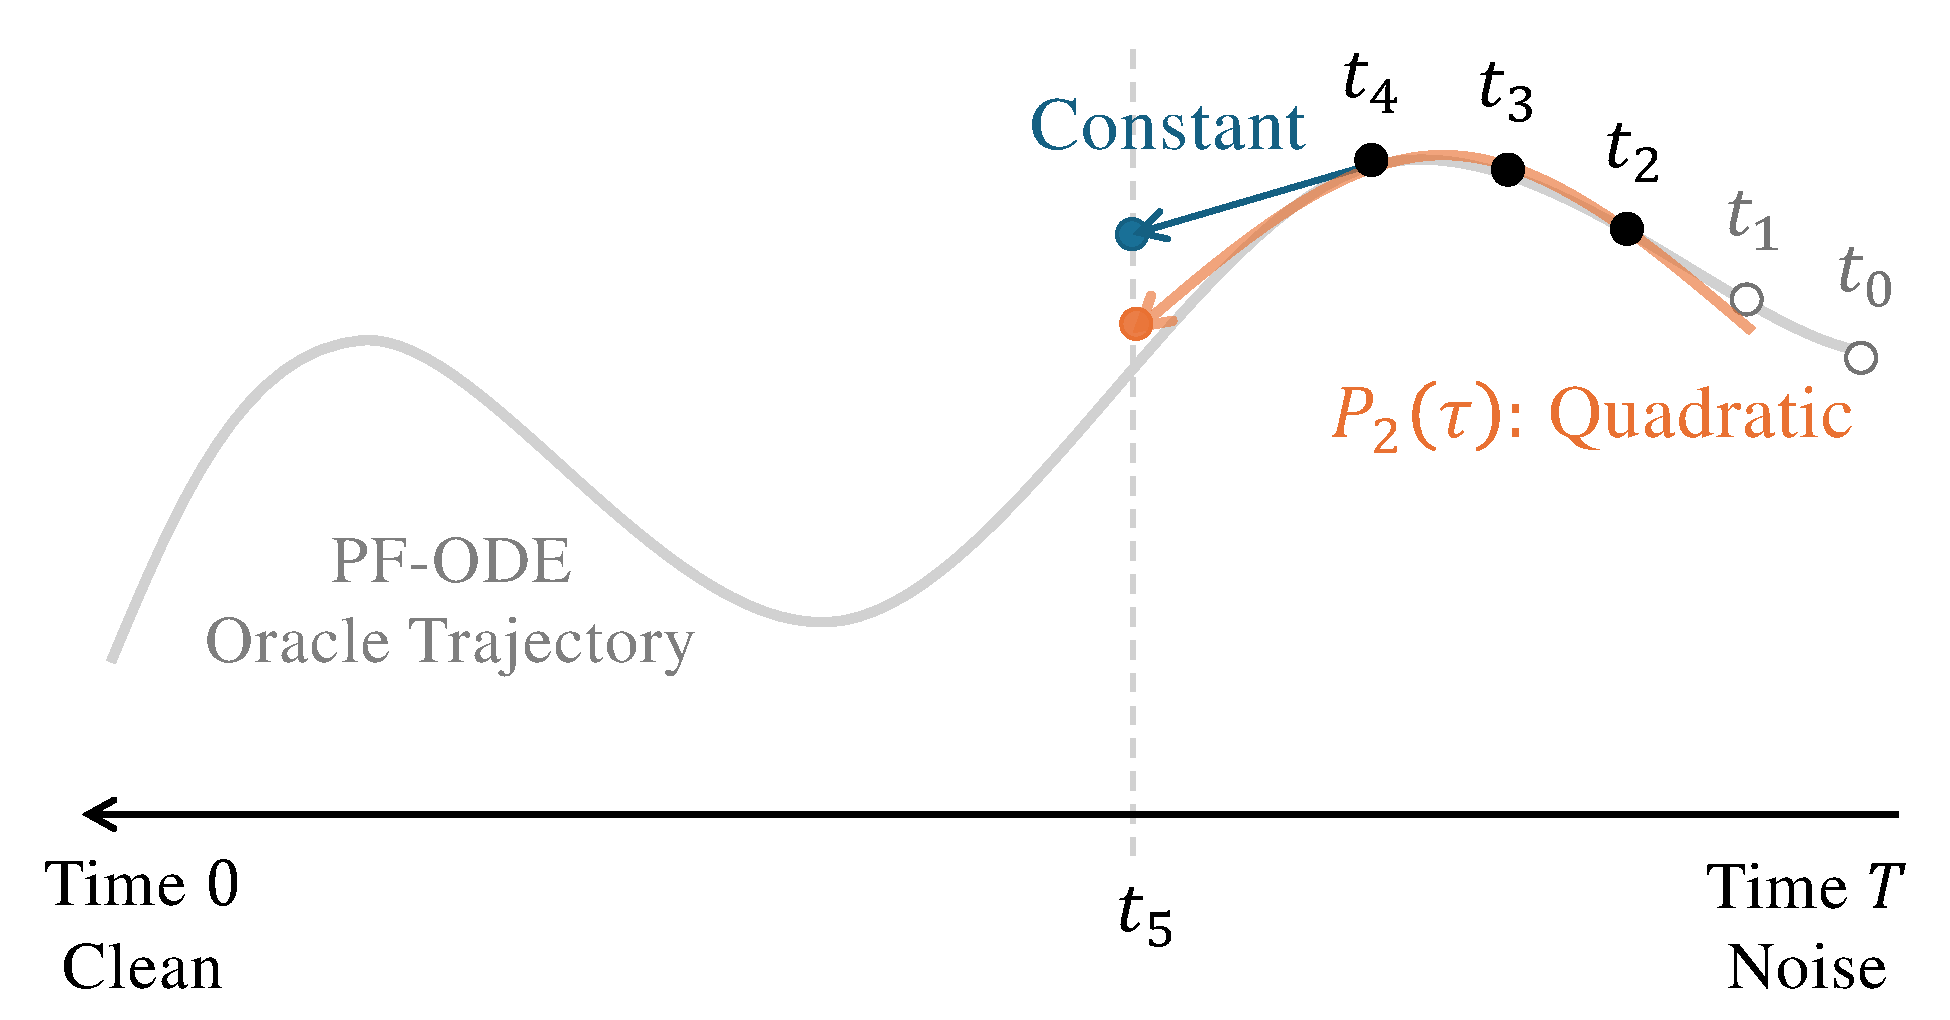
\includegraphics[width=0.85\linewidth]{Images/PartC/DEIS.pdf}
    \caption{\textbfs{DEIS 作为多步骤方法的图示。} 过去的三个锚点位于
$t_2,t_3,t_4$，DEIS 通过模型输出构建二次曲线，并通过以下步骤进行推断
$t_4$ 至 $t_5$。然后将外推多项式与已知的扩散相关权重进行积分，捕获 DDIM 使用的常数近似忽略的神经预测的变化。
\figcredit{由作者创建。}}
    \label{fig:deis_lagrange}
\end{figure}

学位-$n$ 更新需求 $n{+}1$ 锚。当它们可用时（\emph{足够的历史记录}, $i \ge n{+}1$），我们使用完整度-$n$
方案。在最初的步骤中（\emph{历史记录不足}, $i \le n$)，我们使用最高可行度， $i{-}1$，并随着更多锚点可用而增加它。我们下面分别处理这两种情况。


\paragraph{案例一： $i = n+1,\dots,M$ （足够的历史记录）。}
有了足够的历史记录，DEIS 会重用最后一个 $n{+}1$ 模型评估作为锚点，
\[
(\tau_j,\rmY_j) := \bigl(t_{i-1-j}, \bm{\epsilon}_{\bm{\phi}^\times}(\tilde{\rvx}_{t_{i-1-j}},t_{i-1-j})\bigr),
\quad j=0,\dots,n.
\]
查看
$\tau\mapsto\bm{\epsilon}_{\bm{\phi}^\times}(\rvx_\tau,\tau)$
作为沿轨迹的平滑函数，我们构造度数-$n$
拉格朗日多项式
\[
P_n(\tau)
= 
\sum_{j=0}^{n}
\underbrace{\Bigl[\prod_{\substack{k=0\\k\neq j}}^{n}
\frac{\tau - t_{i-1-k}}{\,t_{i-1-j} - t_{i-1-k}\,}\Bigr]}_{=:~\ell_j^{(i)}(\tau)}
\bm{\epsilon}_{\bm{\phi}^\times}\bigl(\tilde{\mathbf x}_{t_{i-1-j}}, t_{i-1-j}\bigr)
\]
通过构造满足 $P_n(\tau_j)=\rmY_j$ 对于每个锚点：
\[
P_n\bigl(\tau_j\bigr)
= \rmY_j =
\bm{\epsilon}_{\bm{\phi}^\times}\bigl(\tilde{\mathbf x}_{t_{i-1-j}}, t_{i-1-j}\bigr),
\quad
 j=0,\ldots,n.
\]
每个 $\ell_j^{(i)}$ 满足
\[
\ell_j^{(i)}\bigl(t_{i-1-m}\bigr)
=
\begin{cases}
1,&m=j,\\
0,&m\neq j.
\end{cases}
\]然后将多项式外推到最新锚点之外
$t_{i-1}$ 新步骤：
\[
\bm{\epsilon}_{\bm{\phi}^\times}(\rvx_\tau,\tau) \approx
P_n(\tau)=\sum_{j=0}^{n}\ell_j^{(i)}(\tau) 
\bm{\epsilon}_{\bm{\phi}^\times}\bigl(\tilde{\rvx}_{t_{i-1-j}}, t_{i-1-j}\bigr), 
\quad \tau \in [t_i,t_{i-1}].
\]
然后我们将 $P_n(\tau)$ 替换为
$\beps_{\bm{\phi}^\times}(\rvx_\tau,\tau)$ 中
指数--积分器公式（\Cref{eq:variation_of_constants}）：
\begin{align*}
\int_{t_{i-1}}^{t_i}
\frac{g^2(\tau)}{2\sigma_\tau}
\mathcal{E}(\tau\to t_i)
\beps_{\bm{\phi}^\times}(\rvx_\tau,\tau)\diff\tau
&\approx
\sum_{j=0}^{n}
\underbrace{
\int_{t_{i-1}}^{t_i}
\frac{g^2(\tau)}{2\sigma_\tau}
\mathcal{E}(\tau\to t_i)
\ell_j^{(i)}(\tau)\diff\tau
}_{=:~C_{i,j}}
\\
&\qquad\cdot
\beps_{\bm{\phi}^\times}
(\tilde\rvx_{t_{i-1-j}},t_{i-1-j}).
\end{align*}
系数
\[
C_{i,j}
:=
\frac{1}{2}
\int_{t_{i-1}}^{t_i}
\frac{g^2(\tau)}{\sigma_\tau}
\mathcal{E}(\tau\to t_i)
\ell_j^{(i)}(\tau)\diff\tau
\]
仅取决于噪声时间表和所选时间网格，因此可以
被预先计算。对于承认合适的反导数的时间表，这些
系数以封闭形式提供；否则可以对其进行评估
数值上达到高精度。

将线性部分与
$\mathcal{E}(t_{i-1}\to t_i)$ 提供 \emph{AB-DEIS-$n$} 更新
\[
\tilde\rvx_{t_i}
=
\mathcal{E}(t_{i-1}\to t_i)\tilde\rvx_{t_{i-1}}
+
\sum_{j=0}^{n}
C_{i,j}
\beps_{\bm{\phi}^\times}
(\tilde\rvx_{t_{i-1-j}},t_{i-1-j}).
\]
对于下面的局部截断语句，让 $h$ 表示一个特征
局部步长并假设相邻步长比率保持有界。下
沿经验模型预测的标准平滑度假设
与计划相关的权重的轨迹和规律性，全历史
度-$n$ 施工有正式订单$n+1$，有一步局部缺陷
$\mathcal O(h^{n+2})$。


\paragraph{案例二：$i=1,\dots,n$（历史记录不足）.}
在初始步骤中，仅 $i$ 过去的模型评估可用。
因此，我们使用所有可用的锚并将多项式次数设置为
$i{-}1$：
\[
P_{i-1}(\tau)
=
\sum_{j=0}^{i-1}
\ell_j^{(i)}(\tau) 
\bm{\epsilon}_{\bm{\phi}^\times}\bigl(\tilde{\mathbf x}_{t_{i-1-j}},  t_{i-1-j}\bigr),
\]
其中 $\ell_j^{(i)}$ 是在时刻节点上建立的次数 $i{-}1$ 的拉格朗日基
$\{t_{i-1}, t_{i-2},\ldots,t_{0}\}$。这匹配所有可用的锚点并且
一旦 $i\ge n{+}1$ 就转换为完整历史公式。

这是多步骤方法的标准热启动情况。第一个
步骤使用常数近似，第二个使用线性外推，
第三个使用二次外推法，依此类推，直到目标度数
$n$ 上市。


\exm{拉格朗日多项式的特例}{
\noindent \textbfs{度$0$（一锚）：}
\[
P_0(\tau) = \bm{\epsilon}_{\bm{\phi}^\times}(\tilde\rvx_{t_{i-1}}, t_{i-1}).
\]
这使得神经预测固定在其起始步骤值，正如
一阶 DDIM 近似。

\medskip
\noindent \textbfs{Degree $1$（两个锚点）：} 拉格朗日多项式是通过两个预先指定的锚点的线性映射。
\[
P_1(\tau)
= 
\underbrace{\frac{\tau - t_{i-2}}{t_{i-1} - t_{i-2}}}_{\displaystyle \ell_{i-1}(\tau)}
\,\bm{\epsilon}_{\bm{\phi}^\times}(\tilde\rvx_{t_{i-1}}, t_{i-1})
 + 
\underbrace{\frac{\tau - t_{i-1}}{t_{i-2} - t_{i-1}}}_{\displaystyle \ell_{i-2}(\tau)}
\,\bm{\epsilon}_{\bm{\phi}^\times}(\tilde\rvx_{t_{i-2}}, t_{i-2}).
\]
这里 $\ell_{i-1}(\tau)$ 和 $\ell_{i-2}(\tau)$ 是拉格朗日基重。
它们满足插值条件：\newline
$P_1(t_{i-1})=\bm{\epsilon}_{\bm{\phi}^\times}(\tilde\rvx_{t_{i-1}}, t_{i-1})$，\newline
$P_1(t_{i-2})=\bm{\epsilon}_{\bm{\phi}^\times}(\tilde\rvx_{t_{i-2}}, t_{i-2})$，
与
$\ell_{i-1}(\tau)+\ell_{i-2}(\tau)=1$。 
}

\paragraph{ AB-DEIS-$n$ 更新摘要。}
结合足够历史记录和热启动案例可以得出
\emph{AB-DEIS-$n$} update\footnote{“AB”指的是 Adams--Bashforth
多步原理，此处应用于指数积分器
公式~\citep{hochbruck2010exponential}.} 这里，$n$ 是目标
多项式次数，使用最多 $n{+}1$ 过去的评估：
\begin{mdframed}
\begin{align*}
\tilde\rvx_{t_i}
= \mathcal{E}(t_{i-1} \to t_i)\,\tilde\rvx_{t_{i-1}}
+ \sum_{j=0}^{\min\{n,\, i-1\}} C_{i,j}\,\beps_{\bm{\phi}^\times}(\tilde\rvx_{t_{i-1-j}},\,t_{i-1-j}),
\end{align*}
有系数
\begin{align*}
C_{i,j}
:= \frac{1}{2} \int_{t_{i-1}}^{t_i}
\frac{g^2(\tau)}{\sigma_\tau}\,\mathcal{E}(\tau \to t_i)\,
\Bigg[\prod_{\substack{k=0\\k\neq j}}^{\min\{n,\, i-1\}}
\frac{\tau - t_{i-1-k}}{\,t_{i-1-j} - t_{i-1-k}\,}\Bigg]\,d\tau.
\end{align*}
\end{mdframed}

当 $i\ge n{+}1$ （足够的历史记录）， $\min\{n,\,i-1\}=n$，以及完整的历史学位-$n$ 步骤存在单步局部截断错误
$\mathcal O(h^{n+2})$ 在上面的假设下，对应的是order方法 $n+1$。热启动期间（$i\le n$)，学位为 $i-1$，所以一步局部截断误差为 $\mathcal O(h^{i+1})$，对应的步骤是正式的命令 $i$。因此，顺序从 $1$ 第一步并达到满订单 $n+1$ 一次 $n+1$ 可以使用锚。与标准多步骤方法一样，低阶热启动步骤本身并不建立全局顺序 -$(n+1)$ 保证；这种保证还需要稳定性和足够准确的起始值。非常大 $n$ 可能会降低数值行为，因为高度外推对锚点间距、存储模型预测中的错误以及稳定性考虑变得越来越敏感。因此，在实践中优选相对小的多项式次数。正如我们将在下一小节中看到的，特殊情况 $n{=}0$ 精确简化为确定性 DDIM，即一阶因式分解指数积分器更新。
\subsection{DDIM = AB-DEIS-0}
\label{sec:ddim-deis}

与 DDIM 的连接在某种程度上变得立即 $n=0$。在这种情况下，拉格朗日多项式是常数，因此 DEIS 在整个下一步中仅使用最新的模型预测。相应的系数简化为
\[
C_{i0} = \frac{1}{2} \int_{t_{i-1}}^{t_{i}} \frac{g^2(\tau)}{\sigma_\tau} \mathcal{E}(\tau \shortrightarrow t_i)   \mathrm{d}\tau.
\]
代入更新公式得到零阶 AB-DEIS 格式：
\begin{align}\label{eq:deis-0}
  \tilde\rvx_{t_{i}} &=  \mathcal{E}(t_{i-1} \shortrightarrow t_{i})\tilde\rvx_{t_{i-1}} + C_{i0} \bm{\epsilon}_{\bm{\phi}^\times}(\tilde\rvx_{t_{i-1}}, t_{i-1})\nonumber\\
  &=e^{\int_{t_{i-1}}^{t_{i}}f(u)\diff u} \tilde\rvx_{t_{i-1}} + \Big( \int_{t_{i-1}}^{t_{i}} \frac{g^2(\tau)}{2\sigma_\tau} e^{\int_{\tau}^{t_{i}}f(u)\diff u}   \mathrm{d}\tau
\Big) \bm{\epsilon}_{\bm{\phi}^\times}(\tilde\rvx_{t_{i-1}}, t_{i-1}).  
\end{align}
这与确定性 DDIM 使用的一阶分解近似完全相同：神经预测固定在
$t_{i-1}$，而已知的积分因子和调度相关系数保留在积分内并在整个步骤中传播。因此，AB-DEIS-0 和 DDIM 不仅仅是一阶等效；他们给出相同的有限步更新。

\proppnp{DDIM = AB-DEIS-0}{ddim-deis}{\Cref{eq:deis-0} 与 DDIM 更新相同 \Cref{eq:ddim-euler}.}

这也阐明了 DEIS 在求解器层次结构中的作用。我们注意到索引``$0$'' 指的是 \emph{多项式次数}，不是数字顺序：AB-DEIS-0 仍然是一阶方法。更高阶的 DEIS 对已知的扩散动力学保持相同的分析处理，但通过从额外的过去模型评估中进行多项式外推来取代这种恒定的预测。因此，DDIM 是 DEIS 多步构造自然延伸的零度基本情况。稍后，在\Cref{subsec:dpm-solver++-multi}，我们会遇到另一条路线
多步扩散求解器；即 DPM-Solver\texttt{++}(2M)。一切从本地开始
对数 SNR 时间中的数据预测进行泰勒展开并循环使用之前的数据
通过后向有限差分模型评估来估计所需的
衍生品。尽管它的表示和推导与
DEIS，两种方法都使用过去的模型评估来捕获
神经预测，无需引入额外的步内阶段。我们返回
到 \Cref{subsec:dpm-deis} 中的这种连接，我们在其中比较两者
结构更加明确。
    
\clearpage
\newpage



\section{\texorpdfstring{DPM-Solver}{DPM-Solver}}\label{sec:dpm}

DPM-Solver~\citep{lu2022dpm} 为经验问题开发高阶求解器
PF-ODE 通过利用与中出现的相同的扩散特定结构
我们对 DDIM 的讨论。中心目标是使用以下方法获得准确的样本
神经网络评估比一阶采样器少得多。原来的
DPM-Solver 专注于噪声预测并构建第一、第二和
三阶单步求解器；后来的扩展，包括
DPM-Solver\texttt{++}~\citep{lu2022dpm2} 和
DPM-Solver-v3~\citep{zheng2023dpm}，进一步开发该系列。

\paragraph{DPM-Solver的高级思想.}
\Cref{sec:revisit-ddim} 中的 DDIM 讨论表明，在
$\beps$-预测，通过保留可以得到一阶更新
在保持神经预测的同时分析已知的扩散时间表
固定在每个步骤上，
\[
\beps_{\bm{\phi}^\times}(\rvx_\tau,\tau)
\approx
\beps_{\bm{\phi}^\times}(\tilde\rvx_s,s).
\]
DPM-Solver~\citep{lu2022dpm} 自然地建立在这个想法之上：而不是
将神经预测视为常数，它寻求高阶
预测如何沿着轨迹变化的近似值。与DEIS一样，
它从 PF-ODE 的半线性 $\beps$ 预测形式开始，
\begin{align}
\label{eq:noise-alpha-sigma}
\frac{\diff \rvx_t}{\diff t}
=
\frac{\alpha_t'}{\alpha_t}\rvx_t
-
\sigma_t
\left(
\frac{\alpha_t'}{\alpha_t}
-
\frac{\sigma_t'}{\sigma_t}
\right)
\beps_{\bphi^\times}(\rvx_t,t),
\end{align}
及其在序言中引入的常数变体表示法。
其关键的附加成分是通过以下方式重新参数化时间
\emph{半对数信噪比}，遵循对数SNR
VDM~\citep{kingma2021variational}的参数化，
\begin{align}
\label{eq:lambda}
\lambda_t
:=
\log\frac{\alpha_t}{\sigma_t}.
\end{align}
该坐标与 DDIM 的调度对齐时钟直接相关
$\rho_t=\sigma_t/\alpha_t$（围绕\Cref{eq:ddim-coordinate-ode-t}讨论）到$\rho_t=e^{-\lambda_t}$，并将
将剩余的模型相关项转化为特别方便的指数形式
加权积分。神经预测的局部泰勒近似
然后可以对 $\lambda$ 进行分析集成，提供系统路线
从一阶 DDIM 更新到高阶扩散求解器。


\subsection{DPM-Solver的见解：通过 Log-SNR} 进行时间重新参数化
\label{subsec:dpm-method}   

我们现在使 \Cref{eq:lambda} 中的对数 SNR 重新参数化变得精确且
推导相应的 PF-ODE 表示。

\paragraph{将变量更改为 PF-ODE 中的对数 SNR。}
假设 $\alpha_t>0$, $\sigma_t>0$，以及 log-SNR 坐标
$\lambda_t$ 在 \Cref{eq:lambda} 在感兴趣的区间上严格单调。然后它承认一个反函数 $t_\lambda(\cdot)$ 满意
\[
t=t_\lambda(\lambda(t)).
\]
对于包含以下内容的时间表 $\sigma_0=0$，一个有 $\lambda_t\to+\infty$ 如
$t\to0$，因此涉及端点的公式 $t=0$ 是通过相应的限制或通过小正端子时间来实现的数值实现。然后我们在中表达状态、时间表和神经预测
$\lambda$-坐标。一顶帽子（$\hat{\cdot}$) 连同 $\lambda$ 表示在此重新参数化的时间坐标中查看相应的数量。更准确地说，定义
\begin{align}
\begin{aligned}
\label{eq:change-of-var-x-epsilon}
\hat{\rvx}_{\lambda}
&:=
\rvx_{t_\lambda(\lambda)},
\\
\alpha_\lambda
&:=
\alpha_{t_\lambda(\lambda)},
\qquad
\sigma_\lambda
:=
\sigma_{t_\lambda(\lambda)},
\\
\hat{\bm{\epsilon}}_{\bm{\phi}^\times}(\rvx,\lambda)
&:=
\bm{\epsilon}_{\bm{\phi}^\times}
\bigl(
\rvx,
t_\lambda(\lambda)
\bigr).
\end{aligned}
\end{align}
因此，沿着经验 PF-ODE 轨迹，
\[
\hat{\bm{\epsilon}}_{\bm{\phi}^\times}
(\hat\rvx_\lambda,\lambda)
=
\bm{\epsilon}_{\bm{\phi}^\times}
\bigl(
\rvx_{t_\lambda(\lambda)},
t_\lambda(\lambda)
\bigr).
\]
自
\[
\frac{\diff\lambda_t}{\diff t}
=
\frac{\alpha_t'}{\alpha_t}
-
\frac{\sigma_t'}{\sigma_t},
\]
PF-ODE \Cref{eq:noise-alpha-sigma} 可以写成
\[
\frac{\diff\rvx_t}{\diff t}
=
\frac{\diff\log\alpha_t}{\diff t}\rvx_t
-
\sigma_t
\frac{\diff\lambda_t}{\diff t}
\bm{\epsilon}_{\bm{\phi}^\times}(\rvx_t,t).
\]
应用链式法则，
\[
\frac{\diff\rvx_t}{\diff t}
=
\frac{\diff\hat\rvx_\lambda}{\diff\lambda}
\frac{\diff\lambda_t}{\diff t},
\qquad
\frac{\diff\log\alpha_t}{\diff t}
=
\frac{\diff\log\alpha_\lambda}{\diff\lambda}
\frac{\diff\lambda_t}{\diff t},
\]
给出对数 SNR 时间的 PF-ODE：
\begin{mdframed}
\begin{align}
\label{eq:diffusion_ode_lambda_eps}
\frac{\diff\hat{\rvx}_\lambda}{\diff\lambda}
=
\frac{\diff\log\alpha_\lambda}{\diff\lambda}
\hat{\rvx}_\lambda
-
\sigma_\lambda
\hat{\bm{\epsilon}}_{\bm{\phi}^\times}
(\hat{\rvx}_\lambda,\lambda).
\end{align}
\end{mdframed}

应用相同的指数积分器（常数变体）技术 \Cref{eq:diffusion_ode_lambda_eps} 给出以下精确解。

\proppp{指数加权精确解}{exp-wgt-exact-sol}{
给定初始值 $\rvx_s$ 当时 $s>0$，精确的经验 PF-ODE 解 $\widetilde\bPsi_{s\to t}(\rvx_s)$ 当时 $t\in(0,s]$ 可以重新表示为
\begin{equation}
\label{eq:analytic_solution}
\widetilde\bPsi_{s\to t}(\rvx_s)
=
\frac{\alpha_t}{\alpha_s}\rvx_s
-
\alpha_t
\int_{\lambda_s}^{\lambda_t}
e^{-\lambda}
\hat{\bm{\epsilon}}_{\bm{\phi}^\times}
(\hat\rvx_\lambda,\lambda)
\diff\lambda.
\end{equation}
当端点满足 $\sigma_0=0$，案例 $t=0$ 通过相应的限制来理解。
}{
来自 \Cref{eq:diffusion_ode_lambda_eps}，与线性项相关的积分因子满足
\[
\exp\left(
\int_{\lambda_s}^{\lambda_t}
\frac{\diff\log\alpha_\lambda}{\diff\lambda}
\diff\lambda
\right)
=
\frac{\alpha_t}{\alpha_s}.
\]
因此，常数变分公式给出
\begin{align*}
\widetilde\bPsi_{s\to t}(\rvx_s)
&=
\frac{\alpha_t}{\alpha_s}\rvx_s
-
\int_{\lambda_s}^{\lambda_t}
\frac{\alpha_t}{\alpha_\lambda}
\sigma_\lambda
\hat{\bm{\epsilon}}_{\bm{\phi}^\times}
(\hat\rvx_\lambda,\lambda)
\diff\lambda
\\
&=
\frac{\alpha_t}{\alpha_s}\rvx_s
-
\alpha_t
\int_{\lambda_s}^{\lambda_t}
e^{-\lambda}
\hat{\bm{\epsilon}}_{\bm{\phi}^\times}
(\hat\rvx_\lambda,\lambda)
\diff\lambda,
\end{align*}
最后一个等式来自
$\sigma_\lambda/\alpha_\lambda=e^{-\lambda}$.
}

关键的数字结果现在已经很明确了。在 $\lambda$-时间，精确解中唯一与模型相关的量出现在里面
\[
\int_{\lambda_s}^{\lambda_t}
e^{-\lambda}
\hat{\bm{\epsilon}}_{\bm{\phi}^\times}
(\hat\rvx_\lambda,\lambda)\diff\lambda.
\]
当模型输出由泰勒多项式局部近似时
$\lambda$，生成的指数加权多项式项可以以封闭形式积分，产生显式的高阶更新系数。因此，正如序言的分解观点一样，已知的时间表依赖性在分析上被保留，而近似集中在神经预测上。

\paragraph{为什么要重新参数化时间？}
对于严格单调 $\lambda(t)$，变量的局部一阶变化给出
\[
|\Delta t|
\approx
\frac{|\Delta\lambda|}{|\lambda'(t)|}.
\]
因此，如果数值网格使用固定步长 $|\Delta\lambda|$，诱导步骤 $t$ 较小，其中 $|\lambda'(t)|$ 更大（即，其中 $\lambda$ 变化迅速 $t$)，以及更大的位置
$|\lambda'(t)|$ 较小。重新参数化本身不会改变 PF-ODE 求解路径；它只改变相同路径的参数化方式：
\[
\frac{\diff \hat\rvx_\lambda}{\diff \lambda}
=
\frac{1}{\lambda'(t)}
\frac{\diff \rvx_t}{\diff t}.
\]
因此，哪里 $|\lambda'(t)|$ 很大，相对于轨迹的变化相同 $t$ 代表更大范围 $\lambda$.更重要的是，$\lambda(t)$ 通过扩散过程衡量进展情况
直接就信号和噪声之间的相对平衡而言。一个固定的
$\Delta\lambda$ 对应于固定的乘法变化
$\alpha_t/\sigma_t$，或相当于对数SNR的固定加性变化，
而相同的 $\Delta t$ 可能对应于非常不同的变化
不同时期的腐败程度。因此，选择数值节点
$\lambda$ 中的统一提供了一种自然的方式来重新分配分辨率
扩散轨迹。原时间精确感应间距
变量 $t$ 取决于所选的噪声表。两个简单的例子
说明这个效果：

\begin{itemize}
\item \textbfs{$(\alpha_t,\sigma_t)=(1-t,t)$.}
这对应于流匹配中常用的线性插值。
然后
\[
\lambda(t)
=
\log\frac{1-t}{t},
\qquad
\lambda'(t)
=
-\frac{1}{t(1-t)},
\]
所以在本地
\[
|\Delta t|
\approx
|\Delta\lambda|\,t(1-t).
\]
因此，$\lambda$ 中的均匀网格会在 $t$ 附近引起非常小的步长
端点 $t\to0$ 和 $t\to1$，以及围绕中间的较大步骤
轨迹。

\item \textbfs{$(\alpha_t,\sigma_t)=(1,t)$.}
这对应于EDM参数化~\citep{karras2022elucidating}
当自变量$t$直接作为噪声水平时
$\sigma_t$。然后
\[
\lambda(t)
=
\log\frac{1}{t},
\qquad
\lambda'(t)
=
-\frac{1}{t},
\]
因此
\[
|\Delta t|
\approx
|\Delta\lambda|\,t.
\]
事实上，$\lambda$ 中的均匀间距意味着
\[
t=e^{-\lambda},
\]
因此相应的噪声水平是几何间隔的。因此，网格
包含小噪声水平（高信噪比）下更精细的绝对间距和更粗的绝对间距
大噪声水平（低信噪比）下的绝对间距。
\end{itemize}



\subsection{利用泰勒展开估计积分}\label{subsec:dpm-method-2} 
DEIS 和 DPM-Solver 利用相同的分解原理，但获得
以不同的方式获取高阶信息。 DEIS 重复使用来自
之前完成的步骤来推断下一个的神经预测
间隔。 DPM-Solver 在 log-SNR 坐标 $\lambda$ 中工作，并且
使用神经预测的局部泰勒展开，以及所需的
从额外评估中获得的高阶信息
当前步骤。我们现在导出这个单步构造。

从 \Cref{eq:analytic_solution} 开始，精确的经验 PF-ODE 流程已初始化
当前数值状态 $\tilde\rvx_s$ 为
\begin{equation}
\label{eqn:analytic_solution_each_step}
\widetilde\bPsi_{s\to t}(\tilde\rvx_s)
=
\frac{\alpha_t}{\alpha_s}\tilde\rvx_s
-
\alpha_t
\int_{\lambda_s}^{\lambda_t}
e^{-\lambda}
\hat{\bm{\epsilon}}_{\bm{\phi}^\times}
(\hat\rvx_\lambda,\lambda)
\diff\lambda,
\end{equation}
其中
$\hat\rvx_{\lambda_s}=\tilde\rvx_s$ 和
$\hat\rvx_\lambda$ 表示相应的精确经验 PF-ODE
当前步骤的轨迹。因此，已知后
与时间表相关的因素已被分析处理，其余的
数值问题是近似
\[
\lambda
\longmapsto
\hat{\bm{\epsilon}}_{\bm{\phi}^\times}
(\hat\rvx_\lambda,\lambda)
\]
在加权积分内。

对于 $n\geq1$，我们扩展了关于 $\lambda_s$ 的神经预测：
\begin{equation*}
\hat{\bm{\epsilon}}_{\bm{\phi}^\times}
(\hat\rvx_\lambda,\lambda)
=
\sum_{k=0}^{n-1}
\frac{(\lambda-\lambda_s)^k}{k!}
\hat{\bm{\epsilon}}_{\bm{\phi}^\times}^{(k)}
(\hat\rvx_{\lambda_s},\lambda_s)
+
\mathcal O\bigl((\lambda-\lambda_s)^n\bigr),
\end{equation*}
其中
\[
\hat{\bm{\epsilon}}_{\bm{\phi}^\times}^{(k)}
(\hat\rvx_\lambda,\lambda)
:=
\frac{\diff^k}{\diff\lambda^k}
\hat{\bm{\epsilon}}_{\bm{\phi}^\times}
(\hat\rvx_\lambda,\lambda)
\]
表示沿经验 PF-ODE 的 $k$-th \emph{ 总导数
轨迹}。特别是，
\[
\frac{\diff}{\diff\lambda}
\hat{\bm{\epsilon}}_{\bm{\phi}^\times}
(\hat\rvx_\lambda,\lambda)
=
\frac{\partial}{\partial\lambda}
\hat{\bm{\epsilon}}_{\bm{\phi}^\times}
(\hat\rvx_\lambda,\lambda)
+
J_{\rvx}
\hat{\bm{\epsilon}}_{\bm{\phi}^\times}
(\hat\rvx_\lambda,\lambda)
\frac{\diff\hat\rvx_\lambda}{\diff\lambda},
\]
因此导数包括对 $\lambda$ 的显式依赖和
通过不断发展的状态的依赖。

将泰勒展开式代入
\Cref{eqn:analytic_solution_each_step} 给出
\begin{mdframed}
\begin{equation}
\label{eq:k-th-expansion}
\widetilde\bPsi_{s\to t}(\tilde\rvx_s)
=
\frac{\alpha_t}{\alpha_s}\tilde\rvx_s
-
\alpha_t
\sum_{k=0}^{n-1}
{\color{cyan}
\hat{\bm{\epsilon}}_{\bm{\phi}^\times}^{(k)}
(\hat\rvx_{\lambda_s},\lambda_s)}
\,{\color{orange}C_k}
+
\mathcal O(h^{n+1}),
\end{equation}
其中
\[
h:=\lambda_t-\lambda_s,
\qquad
{\color{orange}C_k}
:=
\int_{\lambda_s}^{\lambda_t}
e^{-\lambda}
\frac{(\lambda-\lambda_s)^k}{k!}
\diff\lambda.
\]
系数 ${\color{orange}C_k}$ 仅取决于对数 SNR 间隔，并且可以进行分析评估。
\end{mdframed}

如果所需的轨迹导数可用，则删除
$\mathcal O(h^{n+1})$ 余数将给出相应的形式
$n$第-次订单更新。 DPM-Solver 通过从附加模型评估中逼近这些导数来避免显式区分神经网络，如下一小节所述。

\exm{DPM-Solver-1}{
对于 $n=1$，精确的经验流程满足
\[
\widetilde\bPsi_{s\to t}(\tilde\rvx_s)
=
\frac{\alpha_t}{\alpha_s}\tilde\rvx_s
-
\sigma_t
\left(e^h-1\right)
\bm{\epsilon}_{\bm{\phi}^\times}(\tilde\rvx_s,s)
+
\mathcal O(h^2).
\]
放弃 $\mathcal O(h^2)$ 余数定义 DPM-Solver-1：
\begin{align}
\label{eq:dpm-1}
\tilde\rvx_t^{\mathrm{DPM\text{-}Solver\text{-}1}}
:=
\frac{\alpha_t}{\alpha_s}\tilde\rvx_s
-
\sigma_t
\left(e^h-1\right)
\bm{\epsilon}_{\bm{\phi}^\times}(\tilde\rvx_s,s).
\end{align}
这个有限步更新正是确定性DDIM更新，如图所示 \Cref{subsec:ddim=dpm-solver-1}.
}

DPM-Solver-$n$ 与 $n \geq 2$ 需要评估 $k^{\text{th}}$-导数 {\color{cyan}$\hat{\bm{\epsilon}}_{\bm{\phi}^\times}^{(k)}(\hat\rvx_\lambda, \lambda)$} 用于 $k \leq n-1$。然而，在实践中直接计算高阶导数的计算成本很高。 \citet{lu2022dpm} 还提出了这些导数的有效近似方法，这将在下一小节中详细介绍。

 
\subsection{DPM-Solver的实现-$n$}\label{subsec:dpm-n-method} 

\paragraph{DPM-Solver-$n$ 与 $n \geq 2$.}
在实践中，实现高阶 DPM-Solver-$n$ 包含以下内容：
\begin{itemize}
    \item 预计算系数 ${\color{orange}C_k}$;
    \item 近似 $k^{\text{th}}$ 衍生品 {\color{cyan}$\hat{\bm{\epsilon}}_{\bm{\phi}^\times}^{(k)}(\hat\rvx_\lambda,\lambda)$} 用于 $k \leq n-1$ 规避精确高阶导数的昂贵计算——ODE文献中充分研究的一个挑战~\citep{hochbruck2005explicit,luan2021efficient}。一种常见的策略是有限差分近似。
\end{itemize}

我们现在详细阐述前两点。


\subparagraph{预计算 ${\color{orange}C_k}$.}
让 $s$ 和 $t$ 分别表示开始时间和结束时间，定义
$h:=\lambda_t-\lambda_s$。精确经验 PF-ODE 流的泰勒展开式为
\begin{equation}
\label{eq:analytic_expansion}
\widetilde\bPsi_{s\to t}(\rvx_s)
=
\frac{\alpha_t}{\alpha_s}\rvx_s
-
\sigma_t
\sum_{k=0}^{n-1}
h^{k+1}
\varphi_{k+1}(h)
\hat{\bm{\epsilon}}_{\bm{\phi}^\times}^{(k)}
(\hat\rvx_{\lambda_s},\lambda_s)
+
\mathcal O(h^{n+1}),
\end{equation}
其中，对于 $m\geq1$,
\[
\varphi_m(h)
:=
\frac{
e^h-\sum_{j=0}^{m-1}\frac{h^j}{j!}
}{
h^m
},
\qquad
\varphi_m(0):=\frac{1}{m!}.
\]
对于前三种情况，
\begin{align*}
\varphi_1(h)
&=
\frac{e^h-1}{h},
&
\varphi_2(h)
&=
\frac{e^h-h-1}{h^2},
&
\varphi_3(h)
&=
\frac{e^h-\frac{h^2}{2}-h-1}{h^3}.
\end{align*}

\exm{具有精确导数的三阶展开式}{
对于 $n=3$, \Cref{eq:analytic_expansion} 变成
\begin{equation}
\label{eq:example-dpm-solver-3-exact}
\begin{aligned}
\widetilde\bPsi_{s\to t}(\rvx_s)
=
\frac{\alpha_t}{\alpha_s}\rvx_s
&-
\sigma_t
\left(e^h-1\right)
\hat{\bm{\epsilon}}_{\bm{\phi}^\times}
(\hat\rvx_{\lambda_s},\lambda_s)
\\
&-
\sigma_t
\left(e^h-h-1\right)
\hat{\bm{\epsilon}}_{\bm{\phi}^\times}^{(1)}
(\hat\rvx_{\lambda_s},\lambda_s)
\\
&-
\sigma_t
\left(
e^h-\frac{h^2}{2}-h-1
\right)
\hat{\bm{\epsilon}}_{\bm{\phi}^\times}^{(2)}
(\hat\rvx_{\lambda_s},\lambda_s)
+
\mathcal O(h^4).
\end{aligned}
\end{equation}
}



\subparagraph{近似值 {\color{cyan}$\hat{\bm{\epsilon}}_{\bm{\phi}^\times}^{(k)}(\hat\rvx_\lambda,\lambda)$} 用于 $k \leq n-1$.}
对于 $n \geq 2$，遵循单步 ODE 求解器的标准方法~\citep{atkinson2009numerical}, \citet{lu2022dpm} 在当前步骤中使用附加模型评估来近似高阶导数。我们举例说明这个想法 $n=2$.让 $\gamma\in(0,1]$ 指定 log-SNR 间隔中的阶段点
$[\lambda_s,\lambda_t]$。给定 $\tilde\rvx_s$ 处的估计值 $s$，定义
\[
s^{\mathrm{mid}}
=
t_\lambda\left(\lambda_s+\gamma h\right),
\qquad
h:=\lambda_t-\lambda_s.
\]
对于 $\gamma\in(0,1)$ 这是一个内点，而 $\gamma=1$ 对应
到端点 $t$。我们首先使用 DPM-Solver-1 步骤来预测
这个阶段：
\[
\rvx^{\mathrm{mid}}
=
\frac{\alpha_{s^{\mathrm{mid}}}}{\alpha_s}\tilde\rvx_s
-
\sigma_{s^{\mathrm{mid}}}
\left(e^{\gamma h}-1\right)
\bm{\epsilon}_{\bm{\phi}^\times}(\tilde\rvx_s,s).
\]
起始点和阶段点的模型预测之间的差异
然后提供一阶全导数的有限差分近似
沿着轨迹：
\[
\hat{\bm{\epsilon}}_{\bm{\phi}^\times}^{(1)}
(\hat\rvx_{\lambda_s},\lambda_s)
\approx
\frac{
\bm{\epsilon}_{\bm{\phi}^\times}
(\rvx^{\mathrm{mid}},s^{\mathrm{mid}})
-
\bm{\epsilon}_{\bm{\phi}^\times}
(\tilde\rvx_s,s)
}{
\gamma h
}.
\]
将此近似值代入二阶展开式可得
\begin{align}
\label{eq:dpm-solver-2-app}
\begin{aligned}
\widetilde\bPsi_{s\to t}(\tilde\rvx_s)
=
\frac{\alpha_t}{\alpha_s}\tilde\rvx_s
&-
\sigma_t
\left(e^h-1\right)
\bm{\epsilon}_{\bm{\phi}^\times}(\tilde\rvx_s,s)
\\
&-
\frac{\sigma_t}{\gamma h}
\left(e^h-h-1\right)
\left[
\bm{\epsilon}_{\bm{\phi}^\times}
(\rvx^{\mathrm{mid}},s^{\mathrm{mid}})
-
\bm{\epsilon}_{\bm{\phi}^\times}
(\tilde\rvx_s,s)
\right]
+
\mathcal O(h^3).
\end{aligned}
\end{align}
因此，删除 $\mathcal O(h^3)$ 余数会产生二阶
单步更新。

对于中点选择 $\gamma=\tfrac12$，DPM-Solver-2 承认更简单
\Cref{alg:dpm-solver-2} 中的两级形式。此次更新不同于
\Cref{eq:dpm-solver-2-app} 仅由 $\mathcal O(h^3)$ 提供，因此具有
相同的二阶精度。
\begin{algorithm}[H]
    \centering
    \caption{DPM-Solver-2（带$\gamma=\tfrac12$）.}
    \label{alg:dpm-solver-2}
    \begin{algorithmic}[1]
    \Require 初始值$\rvx_T$，时间步$\{t_i\}_{i=0}^M$，模型${\bm{\epsilon}}_{\bm{\phi}^\times}$
        \State $\tilde\rvx_{t_0}\gets\rvx_T$
        \For{$i\gets 1$ 至 $M$}
        \State $h_i \gets \lambda_{t_i}-\lambda_{t_{i-1}}$
        \State $s_i^{\mathrm{mid}}
        \gets
        t_\lambda\left(
        \tfrac{\lambda_{t_{i-1}}+\lambda_{t_i}}{2}
        \right)$
        \State
        $\rvx_i^{\mathrm{mid}}
        \gets
        \tfrac{\alpha_{s_i^{\mathrm{mid}}}}{\alpha_{t_{i-1}}}
        \tilde\rvx_{t_{i-1}}
        -
        \sigma_{s_i^{\mathrm{mid}}}
        \left(e^{h_i/2}-1\right)
        {\bm{\epsilon}}_{\bm{\phi}^\times}
        (\tilde\rvx_{t_{i-1}},t_{i-1})$
        \State
        $\tilde\rvx_{t_i}
        \gets
        \tfrac{\alpha_{t_i}}{\alpha_{t_{i-1}}}
        \tilde\rvx_{t_{i-1}}
        -
        \sigma_{t_i}
        \left(e^{h_i}-1\right)
        {\bm{\epsilon}}_{\bm{\phi}^\times}
        (\rvx_i^{\mathrm{mid}},s_i^{\mathrm{mid}})$
        \EndFor
        \State \Return $\tilde\rvx_{t_M}$
    \end{algorithmic}
\end{algorithm}

\rmkb{
上述有限差分近似为 \emph{total} $\lambda$ 导数
沿着经验 PF-ODE 轨迹的神经预测。低于标准
平滑度假设，
\[
\frac{
\bm{\epsilon}_{\bm{\phi}^\times}
(\rvx^{\mathrm{mid}},s^{\mathrm{mid}})
-
\bm{\epsilon}_{\bm{\phi}^\times}
(\tilde\rvx_s,s)
}{
\gamma h
}
=
\hat{\bm{\epsilon}}_{\bm{\phi}^\times}^{(1)}
(\hat\rvx_{\lambda_s},\lambda_s)
+
\mathcal O(h).
\]
这里，中间状态本身是通过一阶
DPM-Solver-1 步骤，其阶段误差为 $\mathcal O(h^2)$；光滑度下
的模型，这不会改变 $\mathcal O(h)$ 的精度
差商。

在 \Cref{eq:dpm-solver-2-app} 中，该导数近似乘以
\[
e^h-h-1=\mathcal O(h^2),
\]
所以它的诱发误差是$\mathcal O(h^3)$。因此，得到的方法是
对于任何固定的 $\gamma\in(0,1]$ 来说，二阶精度。

这种单步构造需要两次模型求值，分别位于
$(\tilde\rvx_s,s)$以及预测中间阶段
$(\rvx^{\mathrm{mid}},s^{\mathrm{mid}})$。选择$\gamma$不
改变了形式上的二阶精度，但它改变了阶段位置
和误差常数。特别是，$\gamma=\tfrac12$ 排名第二
在 log-SNR 区间的中点进行评估，给出常用的
DPM-Solver-2 的中点版本。
}

\paragraph{实现细节：采样时间步长的选择。}
由于 DPM-Solver 在 log-SNR 时间内构造其局部高阶近似
$\lambda$，自然的选择是将数值节点统一放置在
$\lambda$。对于有限的终止时间 $t_M>0$，这给出
\[
\lambda_{t_i}
=
\lambda_{t_0}
+
\frac{i}{M}
\left(
\lambda_{t_M}-\lambda_{t_0}
\right),
\qquad
i=0,\ldots,M.
\]
如果是 $\sigma_0=0$，则 $\lambda_0=+\infty$，因此在实践中，人们会使用
有限终端 log-SNR 对应于一个小的正时间，其中
由相应的限制或最终去噪步骤处理的端点。虽然推导是在$\lambda$空间中进行的，但是预训练的
型号和时间表 $(\alpha_t,\sigma_t)$ 通常由以下参数化
原始扩散时间$t$。在采样过程中，每个选定的 log-SNR 节点是
因此映射回通过
\[
t_i=t_\lambda(\lambda_{t_i})
\]
每当评估模型或需要进度系数时；
例如，参见 \Cref{alg:dpm-solver-2}。因此，$\lambda$ 用作
数值积分坐标，同时采样器继续评估
原始预训练的扩散模型在其相应的时间标签。



\subsection{DDIM $=$ DPM-Solver-1}
\label{subsec:ddim=dpm-solver-1}

一阶 DPM-Solver精确地恢复 DDIM。两种方法都从一个
相同噪声预测 PF-ODE 的精确积分表示，并使
一步中的相同近似：
\[
\beps_{\bm{\phi}^\times}(\rvx_\tau,\tau)
\approx
\beps_{\bm{\phi}^\times}(\tilde\rvx_s,s).
\]
然后对剩余的与时间表相关的项进行分析积分。
DDIM 直接以派生的时间表对齐形式应用此构造
较早，而 DPM-Solver 首先使用 log-SNR 重写积分
坐标
\[
\lambda_t
=
\log\frac{\alpha_t}{\sigma_t}.
\]
首先，数字时钟的这种变化不会改变常数
模型预测的近似值。因此，两个推导
产生完全相同的有限步更新。

\proppp{DDIM 是 DPM-Solver-1}{ddim-dpm}{
对于固定扩散时间表 $(\alpha_t,\sigma_t)$，确定性 DDIM
\Cref{eq:ddim-euler} 中的更新与 DPM-Solver-1 更新相同
\Cref{eq:dpm-1}。
}{
根据$\lambda$的定义，
\[
\frac{\sigma_s}{\alpha_s}
=
e^{-\lambda_s},
\qquad
\frac{\sigma_t}{\alpha_t}
=
e^{-\lambda_t}.
\]
让
\[
h
=
\lambda_t-\lambda_s.
\]
然后
\[
e^h
=
\frac{\alpha_t/\sigma_t}{\alpha_s/\sigma_s}
=
\frac{\alpha_t\sigma_s}{\sigma_t\alpha_s},
\]
因此
\[
-\sigma_t(e^h-1)
=
\sigma_t
-
\frac{\alpha_t}{\alpha_s}\sigma_s
=
\alpha_t
\left(
\frac{\sigma_t}{\alpha_t}
-
\frac{\sigma_s}{\alpha_s}
\right).
\]
将此恒等式代入 DPM-Solver-1 更新中可得到
\[
\tilde\rvx_t
=
\frac{\alpha_t}{\alpha_s}\tilde\rvx_s
+
\alpha_t
\left(
\frac{\sigma_t}{\alpha_t}
-
\frac{\sigma_s}{\alpha_s}
\right)
\beps_{\bm{\phi}^\times}(\tilde\rvx_s,s),
\]
这正是确定性 DDIM 更新
\Cref{eq:ddim-euler}。
}

因此，DPM-Solver-1 和 DDIM 是同一一阶的两个导数
有限步更新。 log-SNR 坐标变得比第一个更重要
order：高阶 DPM-Solver使用它来近似噪声预测的方式
沿轨迹变化，而不是将该预测视为恒定
整个步骤。


\subsection{ DPM-Solver与龙格库塔型求解器的关系}
\label{subsec:dpm-rk}

DPM-Solver-1 正是 DDIM 更新
(\Cref{subsec:ddim=dpm-solver-1})，所以它的一阶行为已经是
明白了。更高阶的问题是 DPM-Solver 如何改进这一点
一次评估更新。

连接到龙格-库塔 (RK) 方法。欧拉仅使用向量
字段在步骤的开始，而 RK 方法获得额外的
通过 \emph{stages} 的信息，即状态和时间的评估
在当前步骤中生成；参见 \Cref{app:de-solver-examples}。
高阶 DPM-Solver遵循相同的原则：而不是持有一个
神经预测在整个步骤中固定，他们引入了额外的
步内模型评估以捕获其变化。特定扩散
不同之处在于保留了已知的与时间表相关的因素
分析上，而分阶段近似仅适用于学习到的
预测。\paragraph{DPM-Solver-2 与普通中点 RK2.}
我们首先将 DPM-Solver-2 与直接应用于的经典中点 RK2 进行比较
对数 SNR 时间内的完整噪声预测 PF-ODE
\Cref{eq:diffusion_ode_lambda_eps}。为了简洁起见，表示其完整
右侧为 $\rmF(\hat\rvx_\lambda,\lambda)$。

对于中点选择 $\gamma=\tfrac12$，令
\[
\lambda_{\mathrm{mid}}
:=
\lambda_{s^{\mathrm{mid}}}
=
\lambda_s+\frac{h}{2},
\qquad
\alpha_{\mathrm{mid}}
:=
\alpha_{s^{\mathrm{mid}}},
\qquad
\sigma_{\mathrm{mid}}
:=
\sigma_{s^{\mathrm{mid}}},
\]
并缩写
\[
\hat\beps_s
:=
\hat\beps_{\bm{\phi}^\times}(\tilde\rvx_s,\lambda_s)
=
\beps_{\bm{\phi}^\times}(\tilde\rvx_s,s).
\]

经典中点 RK2 给出
\[
\rvx_{\mathrm{mid}}^{\mathrm{RK}}
=
\tilde\rvx_s
+
\frac{h}{2}
\rmF(\tilde\rvx_s,\lambda_s),
\]
随后
\[
\tilde\rvx_t^{\mathrm{RK2}}
=
\tilde\rvx_s
+
h\,
\rmF
\left(
\rvx_{\mathrm{mid}}^{\mathrm{RK}},
\lambda_{\mathrm{mid}}
\right).
\]
因此，普通 RK2 将其两级结构应用于完整的 PF-ODE
速度，包括已知的依赖于时间表的项和神经
预测。

相比之下，\Cref{alg:dpm-solver-2} 中的中点 DPM-Solver-2 首先构建
舞台
\[
\rvx_{\mathrm{mid}}^{\mathrm{DPM2}}
=
\frac{\alpha_{\mathrm{mid}}}{\alpha_s}\tilde\rvx_s
-
\sigma_{\mathrm{mid}}
\left(
e^{h/2}-1
\right)
\hat\beps_s.
\]
将相应的中点预测表示为
\[
\hat\beps_{\mathrm{mid}}^{\mathrm{DPM2}}
:=
\hat\beps_{\bm{\phi}^\times}
\left(
\rvx_{\mathrm{mid}}^{\mathrm{DPM2}},
\lambda_{\mathrm{mid}}
\right),
\]
完整更新是
\[
\tilde\rvx_t^{\mathrm{DPM2}}
=
\frac{\alpha_t}{\alpha_s}\tilde\rvx_s
-
\sigma_t
\left(
e^h-1
\right)
\hat\beps_{\mathrm{mid}}^{\mathrm{DPM2}}.
\]

结构上的差异是直接的。普通中点 RK2 离散化
完整的 PF-ODE 速度，而 DPM-Solver-2 保留已知的
分析扩散依赖演化并使用其两个模型评估
仅用于近似噪声预测的变化。

在标准平滑假设下，两者都是二阶方法
$\lambda$ 时间中的相同经验 PF-ODE。它们的中间状态一般是
$\mathcal O(h^2)$ 有所不同，因此其完整的一步更新
满足
\[
\tilde\rvx_t^{\mathrm{DPM2}}
-
\tilde\rvx_t^{\mathrm{RK2}}
=
\mathcal O(h^3).
\]
因此，DPM-Solver-2 遵循与经典相同的两阶段中点原理
RK2，同时在应用之前利用已知的扩散结构
数值近似。

\paragraph{DPM-Solver-2 与指数中点 RK2.}
更仔细的比较使半线性分解保持在
\Cref{eq:diffusion_ode_lambda_eps} 显式并对待其已知线性部分
分析地。对应\emph{指数中点RK2}构造
首先采用指数欧拉阶段到中点：
\[
\rvx_{\mathrm{mid}}^{\mathrm{ExpRK}}
=
\frac{\alpha_{\mathrm{mid}}}{\alpha_s}\tilde\rvx_s
-
\alpha_{\mathrm{mid}}\sigma_s
\left[
\int_{\lambda_s}^{\lambda_{\mathrm{mid}}}
\frac{1}{\alpha_\lambda}\diff\lambda
\right]
\hat\beps_s.
\]
评估后
\[
\hat\beps_{\mathrm{mid}}^{\mathrm{ExpRK}}
:=
\hat\beps_{\bm{\phi}^\times}
\left(
\rvx_{\mathrm{mid}}^{\mathrm{ExpRK}},
\lambda_{\mathrm{mid}}
\right),
\]
完整的指数中点更新为
\[
\tilde\rvx_t^{\mathrm{ExpRK2}}
=
\frac{\alpha_t}{\alpha_s}\tilde\rvx_s
-
\alpha_t\sigma_{\mathrm{mid}}
\left[
\int_{\lambda_s}^{\lambda_t}
\frac{1}{\alpha_\lambda}\diff\lambda
\right]
\hat\beps_{\mathrm{mid}}^{\mathrm{ExpRK}}.
\]
当线性系数一定时，这些积分系数减小
到显式指数中点 RK2 的常用 $\varphi_1$ 系数。

DPM-Solver-2 使用相同的中点分级原理，但利用了更精细的
噪声预测因子分解
\[
-\sigma_\lambda
\hat\beps_{\bm{\phi}^\times}(\hat\rvx_\lambda,\lambda).
\]
由于 $\sigma_\lambda$ 也可以从扩散表中得知，
DPM-Solver-2 将其保留在积分中，并且仅对神经网络进行分级
预测。因此，它的中点系数和全步系数为
\[
\alpha_{\mathrm{mid}}
\int_{\lambda_s}^{\lambda_{\mathrm{mid}}}
\frac{\sigma_\lambda}{\alpha_\lambda}\diff\lambda
=
\sigma_{\mathrm{mid}}
\left(e^{h/2}-1\right),
\quad \text{and}\quad
\alpha_t
\int_{\lambda_s}^{\lambda_t}
\frac{\sigma_\lambda}{\alpha_\lambda}\diff\lambda
=
\sigma_t
\left(e^h-1\right),
\]
分别恢复\Cref{alg:dpm-solver-2}中的更新。

因此，这三种结构的不同之处在于 RK 的近似值
阶段：
\[
\begin{array}{rl}
\text{\textbfs{Plain RK2:} }
&
\text{stage the complete PF-ODE velocity},
\\[4pt]

\textbf{\textbfs{ExpRK2:} }
&
\begin{aligned}[t]
&\text{propagate the linear part exactly;}\\
&\text{stage the coefficient-weighted residual }
\sigma_\lambda\hat\beps_{\bm{\phi}^\times},
\end{aligned}
\\[6pt]

\text{\textbfs{DPM-Solver-2:} }
&
\text{also retain }\sigma_\lambda\text{ analytically and stage only }
\hat\beps_{\bm{\phi}^\times}.
\end{array}
\]

指数 RK 和 DPM 中点阶段的不同之处在于
\[
\rvx_{\mathrm{mid}}^{\mathrm{DPM2}}
-
\rvx_{\mathrm{mid}}^{\mathrm{ExpRK}}
=
-
\alpha_{\mathrm{mid}}
\left[
\int_{\lambda_s}^{\lambda_{\mathrm{mid}}}
\frac{\sigma_\lambda-\sigma_s}{\alpha_\lambda}
\diff\lambda
\right]
\hat\beps_s
=
\mathcal O(h^2).
\]
对于完整的步骤，泰勒展开式为
$\lambda_{\mathrm{mid}}$ 给出
\[
\int_{\lambda_s}^{\lambda_t}
\frac{\sigma_\lambda-\sigma_{\mathrm{mid}}}{\alpha_\lambda}
\diff\lambda
=
\mathcal O(h^3),
\]
而神经预测的平滑度给出
\[
\hat\beps_{\mathrm{mid}}^{\mathrm{DPM2}}
-
\hat\beps_{\mathrm{mid}}^{\mathrm{ExpRK}}
=
\mathcal O(h^2).
\]
因此，
\[
\tilde\rvx_t^{\mathrm{DPM2}}
-
\tilde\rvx_t^{\mathrm{ExpRK2}}
=
\mathcal O(h^3).
\]
因此，DPM-Solver-2 和指数中点 RK2 通过二阶一致，
但 DPM-Solver-2 保留了一个额外的分析已知量，
$\sigma_\lambda$，加权积分里面。\rmkb{
上面的讨论涉及噪声预测公式，其中
DPM-Solver 已导出。如果预训练模型使用另一个预测
参数化，其输出可以逐点转换为噪声预测
在每个阶段通过\Cref{eq:predictions-equivalence}。就像 \Cref{subsec:ddim-classical-euler} 中的 DDIM 案例一样，这不应该是
与直接将经典 RK 方法应用于原始预测相混淆
field：逐点转换和有限步离散化是分开的
操作。
}

\msgu{DPM-Solver和龙格--库塔方法}{}{
DPM-Solver 结合了 Runge--Kutta 的步内分级原理
对已知扩散动力学进行分析处理的方法。
DPM-Solver-1 正是 DDIM，而高阶 DPM-Solvers 使用额外的
步内评估以捕获神经预测的变化。
与经典 RK 方法的联系是结构性的，而不是等式的
有限步公式：DPM-Solver 保留了已知的扩散相关
在近似学习的预测之前分析权重。
}


\clearpage
\newpage

\section{\texorpdfstring{DPM-Solver\texttt{++}}{DPM-Solver\texttt{++}}}\label{sec:dpm++}


\subsection{从 DPM-Solver到 DPM-Solver\texttt{++} 用于引导采样}

DPM-Solver\texttt{++}~\citep{lu2022dpm2} 的开发是为了改进
强指导下的高阶抽样。在这个制度下，有两个实际的
出现困难。首先，大制导尺度可以放大模型输出
及其导数，缩小高阶求解器的收敛区域
并且需要更小的数值步长。其次，引导预测可以
将最终解决方案驱动到训练数据表示的范围之外，
导致中讨论的训练-测试不匹配
\Cref{ch:guidance}。

DPM-Solver\texttt{++} 通过两种互补的方式解决这些问题。它
使用数据预测重新表述扩散 ODE，其中数据空间
可以应用动态阈值等校正，并且它开发了
多步变体，重用以前的模型评估以获得更小的
固定 NFE 预算下的有效步长。我们首先推导出
数据预测公式，然后介绍其单步和多步
二阶求解器。


\subsection{DPM-Solver\texttt{++}的方法论}

DPM-Solver\texttt{++} 保持对数 SNR 坐标 $\lambda$ 引入
DPM-Solver，而是通过数据预测来表达经验 PF-ODE
比噪声预测。回想一下 \Cref{eq:predictions-equivalence} 中的内容
\[
\beps_{\bm{\phi}^\times}(\rvx_t,t)
=
\frac{
\rvx_t-\alpha_t\rvx_{\bm{\phi}^\times}(\rvx_t,t)
}{
\sigma_t
}.
\]
将此关系代入噪声预测精确解中
\Cref{eq:analytic_solution} 给出等效的数据预测形式
\begin{equation}
\label{eq:dpmpp-data-exact}
\widetilde\bPsi_{s\to t}(\rvx_s)
=
\frac{\sigma_t}{\sigma_s}\rvx_s
+
\sigma_t
\int_{\lambda_s}^{\lambda_t}
e^\lambda
\hat{\rvx}_{\bm{\phi}^\times}
(\hat\rvx_\lambda,\lambda)
\diff\lambda,
\end{equation}
其中，在 \Cref{eq:change-of-var-x-epsilon} 之后，我们定义
$\lambda$-参数化数据预测字段
\[
\hat{\rvx}_{\bm{\phi}^\times}
(\rvx,\lambda)
:=
\rvx_{\bm{\phi}^\times}
\bigl(
\rvx,
t_\lambda(\lambda)
\bigr).
\]
因此，沿着经验 PF-ODE 轨迹，
\[
\hat{\rvx}_{\bm{\phi}^\times}
(\hat\rvx_\lambda,\lambda)
=
\rvx_{\bm{\phi}^\times}
\bigl(
\rvx_{t_\lambda(\lambda)},
t_\lambda(\lambda)
\bigr).
\]因此，该结构与 DPM-Solver 完全对偶：已知
依赖于时间表的演化是通过分析处理的，而唯一的
剩余积分内的模型相关量现在是数据
预测。 DPM-Solver\texttt{++} 开发了两个二阶实现
这个确切的形式：

\begin{itemize}
    \item \textbfs{单步求解器、DPM-Solver\texttt{++}(2S).}
    在中间阶段使用额外的模型评估
    当前步骤，类似于 DPM-Solver-2 的分阶段构建。

    \item \textbfs{多步求解器、DPM-Solver\texttt{++}(2M).}
    重用前两个已完成步骤的数据预测。之后
    热启动，每一步只需要评估一个新模型。
\end{itemize}

\rmkb{
如果没有阈值处理，将模型输出转换为数据预测是一个
相同经验 PF-ODE 的逐点代数重新表达。数值
尽管如此，方法仍然可以改变，因为有限步近似现在是
应用于数据预测而不是噪声预测。如果
使用阈值，它是对模型输出的额外修改
并且应该与下面的数字顺序分析分开看待。
}

\subsection{DPM-Solver\texttt{++} 泰勒展开式单步}
\label{subsec:dpm-solver++-single}

按照 \Cref{subsec:dpm-method-2} 中的 DPM-Solver构建，
DPM-Solver\texttt{++} 沿着经验近似数据预测
通过对数 SNR 时间内局部泰勒展开的轨迹。对于 $k\geq0$，表示
其沿经验 PF-ODE 轨迹的 $k$ 全导数为
\[
\hat{\rvx}_{\bm{\phi}^\times}^{(k)}
(\hat\rvx_\lambda,\lambda)
:=
\frac{\diff^k}{\diff\lambda^k}
\hat{\rvx}_{\bm{\phi}^\times}
(\hat\rvx_\lambda,\lambda).
\]

对于从 $t_{i-1}$ 到 $t_i$ 的一步，设 $h_i
:=
\lambda_{t_i}-\lambda_{t_{i-1}}
>0$。关于 $\lambda_{t_{i-1}}$ 的泰勒展开给出
\[
\hat{\rvx}_{\bm{\phi}^\times}
(\hat\rvx_\lambda,\lambda)
=
\sum_{k=0}^{n-1}
\frac{
(\lambda-\lambda_{t_{i-1}})^k
}{
k!
}
\hat{\rvx}_{\bm{\phi}^\times}^{(k)}
\bigl(
\hat\rvx_{\lambda_{t_{i-1}}},
\lambda_{t_{i-1}}
\bigr)
+
\mathcal O
\bigl(
(\lambda-\lambda_{t_{i-1}})^n
\bigr).
\]
将此扩展代入 \Cref{eq:dpmpp-data-exact} 得到
\begin{align}
\label{eq:dpmpp-taylor-expansion}
\widetilde\bPsi_{t_{i-1}\to t_i}
(\tilde\rvx_{t_{i-1}})
=
\frac{\sigma_{t_i}}{\sigma_{t_{i-1}}}
\tilde\rvx_{t_{i-1}}
+
\alpha_{t_i}
\sum_{k=0}^{n-1}
h_i^{k+1}
\varphi_{k+1}(-h_i)
\hat{\rvx}_{\bm{\phi}^\times}^{(k)}
\bigl(
\hat\rvx_{\lambda_{t_{i-1}}},
\lambda_{t_{i-1}}
\bigr)
+
\mathcal O(h_i^{n+1}),
\end{align}
其中 $\varphi_m$ 在 \Cref{eq:analytic_expansion} 中定义。这里我们使用了
\[
\int_{\lambda_{t_{i-1}}}^{\lambda_{t_i}}
e^\lambda
\frac{
(\lambda-\lambda_{t_{i-1}})^k
}{
k!
}
\diff\lambda
=
e^{\lambda_{t_i}}
h_i^{k+1}
\varphi_{k+1}(-h_i),
\]
与...一起
$\sigma_{t_i}e^{\lambda_{t_i}}=\alpha_{t_i}$。

对于 $n=1$，删除 $\mathcal O(h_i^2)$ 余数给出
\[
\tilde\rvx_{t_i}
=
\frac{\sigma_{t_i}}{\sigma_{t_{i-1}}}
\tilde\rvx_{t_{i-1}}
+
\alpha_{t_i}
\left(
1-e^{-h_i}
\right)
\rmD_{i-1},
\qquad
\rmD_{i-1}
:=
\rvx_{\bm{\phi}^\times}
(\tilde\rvx_{t_{i-1}},t_{i-1}),
\]
这正是数据预测形式的确定性 DDIM 更新。

对于 $n=2$，一阶全导数使用附加函数来近似
步内阶段。对于中点选择，定义
\[
s_i^{\mathrm{mid}}
:=
t_\lambda
\left(
\lambda_{t_{i-1}}+\frac{h_i}{2}
\right).
\]
一阶 DPM-Solver\texttt{++} 步骤预测中点状态
\[
\rvu_i
=
\frac{
\sigma_{s_i^{\mathrm{mid}}}
}{
\sigma_{t_{i-1}}
}
\tilde\rvx_{t_{i-1}}
+
\alpha_{s_i^{\mathrm{mid}}}
\left(
1-e^{-h_i/2}
\right)
\rmD_{i-1},
\]
我们评估
\[
\rmD_i^{\mathrm{mid}}
:=
\rvx_{\bm{\phi}^\times}
(\rvu_i,s_i^{\mathrm{mid}}).
\]
然后，中点 DPM-Solver\texttt{++}(2S) 更新特别采用
简单的形式
\[
\tilde\rvx_{t_i}
=
\frac{\sigma_{t_i}}{\sigma_{t_{i-1}}}
\tilde\rvx_{t_{i-1}}
+
\alpha_{t_i}
\left(
1-e^{-h_i}
\right)
\rmD_i^{\mathrm{mid}}.
\]
与中点 DPM-Solver-2 一样，这种简化的两阶段更新不同于
直接二阶泰勒/有限差分构造仅通过
$\mathcal O(h_i^3)$ 因此保留了二阶精度。

这会产生单步 DPM-Solver\texttt{++} 施工。当 $n=1$，它精确地简化为数据预测形式的确定性 DDIM 更新。当 $n=2$，近似第一个总数 $\lambda$-使用额外的步内模型评估的导数给出
\emph{DPM-Solver\texttt{++}(2S)}，DPM-Solver-2 的数据预测对应项 \Cref{alg:dpm-solver-2}。其中点实现总结为 \Cref{alg:dpmpp-2s-mid}.
\begin{algorithm}[H]
    \centering
    \caption{DPM-Solver\texttt{++}（2S）：中点特殊情况。}
    \label{alg:dpmpp-2s-mid}
    \begin{algorithmic}[1]
    \Require 初始值 $\rvx_T$，时间步长 $\{t_i\}_{i=0}^M$，数据预测模型 $\rvx_{\bphi^\times}$

    \State $\tilde\rvx_{t_0}\gets\rvx_T$
    \State $\lambda_{t_i}\gets\log(\alpha_{t_i}/\sigma_{t_i})$
    用于 $i=0,\ldots,M$
    \State
    $\rmD_0
    \gets
    \rvx_{\bphi^\times}(\tilde\rvx_{t_0},t_0)$
    \Comment{缓存启动预测}

    \For{$i\gets1$ \textbf{至} $M$}
        \State
        $h_i
        \gets
        \lambda_{t_i}-\lambda_{t_{i-1}}$

        \State
        $s_i^{\mathrm{mid}}
        \gets
        t_\lambda
        \left(
        \tfrac{\lambda_{t_{i-1}}+\lambda_{t_i}}{2}
        \right)$

        \State
        $\rvu_i
        \gets
        \tfrac{\sigma_{s_i^{\mathrm{mid}}}}{\sigma_{t_{i-1}}}
        \tilde\rvx_{t_{i-1}}
        +
        \alpha_{s_i^{\mathrm{mid}}}
        \left(
        1-e^{-h_i/2}
        \right)
        \rmD_{i-1}$
        \Comment{预测中点阶段}

        \State
        $\rmD_i^{\mathrm{mid}}
        \gets
        \rvx_{\bphi^\times}
        (\rvu_i,s_i^{\mathrm{mid}})$
        \Comment{在中点评估}

        \State
        $\tilde\rvx_{t_i}
        \gets
        \tfrac{\sigma_{t_i}}{\sigma_{t_{i-1}}}
        \tilde\rvx_{t_{i-1}}
        +
        \alpha_{t_i}
        \left(
        1-e^{-h_i}
        \right)
        \rmD_i^{\mathrm{mid}}$

        \If{$i<M$}
            \State
            $\rmD_i
            \gets
            \rvx_{\bphi^\times}
            (\tilde\rvx_{t_i},t_i)$
            \Comment{下一步的缓存}
        \EndIf
    \EndFor

    \State \Return $\tilde\rvx_{t_M}$
    \end{algorithmic}
\end{algorithm}


\subsection{DPM-Solver\texttt{++} 按回收历史记录进行多步骤}
\label{subsec:dpm-solver++-multi}

DPM-Solver\texttt{++}（2S）通过引入额外的模型评估获得二阶信息 \emph{在当前步骤内}。 DPM-Solver\texttt{++}(2M) 采用不同的路线：它重用之前已完成步骤的模型预测来估计相同的局部变化。初始化后，每个步骤仅需要一次新模型评估，从而在相同的 NFE 预算下允许更多、因此更小的数值步骤。这在强指导下特别有用，因为大的步长会降低数值稳定性。这个想法很简单。回想一下，二阶展开式
\Cref{eq:dpmpp-taylor-expansion} 需要当前数据预测及其相对于的一阶全导数 $\lambda$。单步方法使用新的步内阶段来估计该导数；相反，多步方法根据模型预测的最近历史记录来估计它。对于第一步，没有可用的历史记录，因此我们使用一阶数据预测更新进行初始化
\[
\tilde\rvx_{t_1}
=
\frac{\sigma_{t_1}}{\sigma_{t_0}}
\tilde\rvx_{t_0}
+
\alpha_{t_1}
\left(
1-e^{-h_1}
\right)
\rmD_0,
\qquad
\rmD_0
:=
\rvx_{\bm{\phi}^\times}
(\tilde\rvx_{t_0},t_0).
\]
这正是数据预测形式的确定性 DDIM 更新。一旦两个完成的步骤预测可用，对于 $i\geq2$ 定义
\[
\rmD_{i-1}
:=
\rvx_{\bm{\phi}^\times}
(\tilde\rvx_{t_{i-1}},t_{i-1}),
\qquad
\rmD_{i-2}
:=
\rvx_{\bm{\phi}^\times}
(\tilde\rvx_{t_{i-2}},t_{i-2}).
\]
保留前两项
\Cref{eq:dpmpp-taylor-expansion} 给出
\begin{align*}
\widetilde\bPsi_{t_{i-1}\to t_i}
(\tilde\rvx_{t_{i-1}})
=
\frac{\sigma_{t_i}}{\sigma_{t_{i-1}}}
\tilde\rvx_{t_{i-1}}
&+
\alpha_{t_i}
\left(
1-e^{-h_i}
\right)
\rmD_{i-1}
\\
&+
\alpha_{t_i}
\left(
h_i-1+e^{-h_i}
\right)
\hat{\rvx}_{\bm{\phi}^\times}^{(1)}
\bigl(
\hat\rvx_{\lambda_{t_{i-1}}},
\lambda_{t_{i-1}}
\bigr)
+
\mathcal O(h_i^3).
\end{align*}
因此，二阶更新所需的唯一额外数量是第一个总计 $\lambda$-数据预测的导数。不是在新的中间阶段评估模型，
DPM-Solver\texttt{++}(2M) 根据之前的结果估计此导数
已完成的步骤：
\[
\hat{\rvx}_{\bm{\phi}^\times}^{(1)}
\bigl(
\hat\rvx_{\lambda_{t_{i-1}}},
\lambda_{t_{i-1}}
\bigr)
\approx
\frac{
\rmD_{i-1}-\rmD_{i-2}
}{
h_{i-1}
}.
\]
在标准平滑度假设下，这种后向差分存在误差
$\mathcal O(h_{i-1})$。将其代入二阶展开式并
收集两个预测项给出
\[
\tilde\rvx_{t_i}^{\mathrm{poly}}
=
\frac{\sigma_{t_i}}{\sigma_{t_{i-1}}}
\tilde\rvx_{t_{i-1}}
+
\alpha_{t_i}
\left(
1-e^{-h_i}
\right)
\rmD_i^{\mathrm{poly}},
\]
其中
\[
\rmD_i^{\mathrm{poly}}
:=
\rmD_{i-1}
+
\frac{\beta(h_i)}{h_{i-1}}
\left(
\rmD_{i-1}-\rmD_{i-2}
\right),
\qquad
\beta(h)
:=
\frac{
h-1+e^{-h}
}{
1-e^{-h}
}.
\]
当连续步长比率保持有界时，此加权多步更新
具有一步局部缺陷 $\mathcal O(h_i^3)$。

\paragraph{实用DPM-Solver\texttt{++}(2M)更新.}
上面的表达式已经是一个有效的二阶多步构造。
DPM-Solver\texttt{++}(2M) 使用稍微简单的系数，保留
相同的顺序。自从
\[
\beta(h)
=
\frac{h}{2}
+
\frac{h^2}{12}
+
\mathcal O(h^3),
\]
定义步长比
\[
r_i
:=
\frac{h_i}{h_{i-1}}
\]
并将 $\rmD_i^{\mathrm{poly}}$ 替换为
\[
\rmD_i^{\mathrm{sim}}
:=
\rmD_{i-1}
+
\frac{r_i}{2}
\left(
\rmD_{i-1}-\rmD_{i-2}
\right).
\]
等价地，
\[
\rmD_i^{\mathrm{sim}}
=
\left(
1+\frac{r_i}{2}
\right)\rmD_{i-1}
-
\frac{r_i}{2}\rmD_{i-2}.
\]
解释很简单：两个最新的模型预测
告诉我们数据预测变化的局部方向，以及
$\rmD_i^{\mathrm{sim}}$ 将该趋势推断到当前步骤。

在相同的平滑度和有界步长比假设下，
\[
\rmD_i^{\mathrm{poly}}
-
\rmD_i^{\mathrm{sim}}
=
\mathcal O(h_i^2).
\]
自从
\[
\alpha_{t_i}
\left(
1-e^{-h_i}
\right)
=
\mathcal O(h_i),
\]
这种简化仅通过以下方式更改状态更新
$\mathcal O(h_i^3)$。因此，它保留了二阶精度，给出
实用DPM-Solver\texttt{++}(2M)更新
\begin{mdframed}
\[
\tilde\rvx_{t_i}
=
\frac{\sigma_{t_i}}{\sigma_{t_{i-1}}}
\tilde\rvx_{t_{i-1}}
+
\alpha_{t_i}
\left(
1-e^{-h_i}
\right)
\rmD_i^{\mathrm{sim}}.
\]
\end{mdframed}

计算完 $\tilde\rvx_{t_i}$ 后，模型在新的
状态，
\[
\rmD_i
=
\rvx_{\bm{\phi}^\times}
(\tilde\rvx_{t_i},t_i),
\]
并且该预测被缓存以供下一步使用。因此，在热启动后，
每个 DPM-Solver\texttt{++}(2M) 步骤仅需要一次新模型评估。

\rmkb{
对于统一的 log-SNR 步骤，$r_i=1$，所以
\[
\rmD_i^{\mathrm{sim}}
=
\frac{3}{2}\rmD_{i-1}
-
\frac{1}{2}\rmD_{i-2}.
\]
系数 $(\frac32,-\frac12)$ 是熟悉的 AB2 外推法
\emph{模型预测}的权重。完整的
DPM-Solver\texttt{++}(2M) 更新仍然不是简单的 AB2：已知
扩散依赖性因子
$\alpha_{t_i}(1-e^{-h_i})$ 被保留分析。
}

完整的热启动和两步程序总结于
\Cref{alg:dpmpp-2m}。与的主要区别
DPM-Solver\texttt{++}(2S) 是二阶信息的来源：
2S 从当前步骤内的附加阶段获取它，而 2M
从之前完成的步骤中回收模型评估。


\begin{algorithm}[H]
    \centering
    \caption{DPM-Solver\texttt{++}(2M).}
    \label{alg:dpmpp-2m}
    \begin{algorithmic}[1]
    \Require 初始值$\rvx_T$，时间步长$\{t_i\}_{i=0}^M$，
    数据预测模型 $\rvx_{\bphi^\times}$

    \State $\tilde\rvx_{t_0}\gets\rvx_T$
    \State $\lambda_{t_i}\gets\log(\alpha_{t_i}/\sigma_{t_i})$
    适用于$i=0,\ldots,M$
    \State
    $\rmD_0
    \gets
    \rvx_{\bphi^\times}
    (\tilde\rvx_{t_0},t_0)$
    \Comment{缓存启动预测}

    \Statex
    \noindent\textbfs{案例一、热启动（$i=1$）}

    \State
    $h_1
    \gets
    \lambda_{t_1}-\lambda_{t_0}$

    \State
    $\tilde\rvx_{t_1}
    \gets
    \tfrac{\sigma_{t_1}}{\sigma_{t_0}}
    \tilde\rvx_{t_0}
    +
    \alpha_{t_1}
    \left(
    1-e^{-h_1}
    \right)
    \rmD_0$
    数据预测中的\Comment{DDIM}

    \If{$M>1$}
        \State
        $\rmD_1
        \gets
        \rvx_{\bphi^\times}
        (\tilde\rvx_{t_1},t_1)$
        \Comment{多步更新缓存}
    \EndIf\Statex
    \noindent\textbfs{案例二。两步多步更新（$i\geq2$）}

    \For{$i\gets2$ \textbf{至} $M$}
        \State
        $h_i
        \gets
        \lambda_{t_i}-\lambda_{t_{i-1}}$

        \State
        $r_i
        \gets
        h_i/h_{i-1}$
        \Comment{步长比}

        \State
        $\rmD_i^{\mathrm{sim}}
        \gets
        \left(
        1+\tfrac12 r_i
        \right)
        \rmD_{i-1}
        -
        \tfrac12 r_i
        \rmD_{i-2}$

        \State
        $\tilde\rvx_{t_i}
        \gets
        \tfrac{\sigma_{t_i}}{\sigma_{t_{i-1}}}
        \tilde\rvx_{t_{i-1}}
        +
        \alpha_{t_i}
        \left(
        1-e^{-h_i}
        \right)
        \rmD_i^{\mathrm{sim}}$

        \If{$i<M$}
            \State
            $\rmD_i
            \gets
            \rvx_{\bphi^\times}
            (\tilde\rvx_{t_i},t_i)$
            \Comment{one新型号来电；下一步缓存}
        \EndIf
    \EndFor

    \State \Return $\tilde\rvx_{t_M}$
    \end{algorithmic}
\end{algorithm}

\subsection{ DPM-Solver\texttt{++}(2M) 与 DEIS} 的关系
\label{subsec:dpm-deis}

DPM-Solver\texttt{++}(2M) 和 DEIS 使用相同的基本多步思想：
重用之前完成的步骤中的模型预测来近似
神经预测在下一个时间间隔内发生变化，同时保持已知的
依赖于扩散的权重分析。区别在于表示
应用了这个想法。 DEIS 是早期使用噪声预测制定的
在原始扩散时间内，而 DPM-Solver\texttt{++}(2M) 使用数据
以对数 SNR 时间进行预测。

为了直接暴露连接，我们可以应用 DEIS 多项式
精确数据预测积分的外推原理
DPM-Solver\texttt{++}。回想一下
\[
\widetilde\bPsi_{t_{i-1}\to t_i}
(\tilde\rvx_{t_{i-1}})
=
\frac{\sigma_{t_i}}{\sigma_{t_{i-1}}}
\tilde\rvx_{t_{i-1}}
+
\sigma_{t_i}
\int_{\lambda_{t_{i-1}}}^{\lambda_{t_i}}
e^\lambda
\hat{\rvx}_{\bm{\phi}^\times}
(\hat\rvx_\lambda,\lambda)
\diff\lambda.
\]
已知重量 $e^\lambda$ 已进行分析处理。唯一的
因此，必须在步骤中近似的数量是数据
预测
\[
\lambda
\longmapsto
\hat{\rvx}_{\bm{\phi}^\times}
(\hat\rvx_\lambda,\lambda).
\]

使用两个最近缓存的预测
$\rmD_{i-2}$ 和 $\rmD_{i-1}$，最简单的非常数近似是
通过这两个锚点的唯一仿射多项式。在拉格朗日形式中，
\[
P_1(\lambda)
=
\frac{
\lambda-\lambda_{t_{i-2}}
}{
h_{i-1}
}
\rmD_{i-1}
-
\frac{
\lambda-\lambda_{t_{i-1}}
}{
h_{i-1}
}
\rmD_{i-2}.
\]
相同的多项式可以围绕最近的更透明地编写
锚定为
\[
P_1(\lambda)
=
\rmD_{i-1}
+
\frac{
\lambda-\lambda_{t_{i-1}}
}{
h_{i-1}
}
\left(
\rmD_{i-1}-\rmD_{i-2}
\right).
\]
第一个表达式是拉格朗日形式，第二个表达式是
\emph{same} 仿射多项式的后向牛顿形式。因此，拉格朗日
插值和后向差分不是数值上的不同
这里的近似值；它们只是同一事物的两种表示
双锚点外推法。

在 DPM-Solver\texttt{++} 积分内应用此外推法可得出
\[
\tilde\rvx_{t_i}^{\mathrm{poly}}
=
\frac{\sigma_{t_i}}{\sigma_{t_{i-1}}}
\tilde\rvx_{t_{i-1}}
+
\sigma_{t_i}
\int_{\lambda_{t_{i-1}}}^{\lambda_{t_i}}
e^\lambda
P_1(\lambda)
\diff\lambda.
\]
由于重量 $e^\lambda$ 已知，因此所需的两个矩可以为
准确评估：
\[
\sigma_{t_i}
\int_{\lambda_{t_{i-1}}}^{\lambda_{t_i}}
e^\lambda\diff\lambda
=
\alpha_{t_i}
\left(
1-e^{-h_i}
\right),
\]
和
\[
\sigma_{t_i}
\int_{\lambda_{t_{i-1}}}^{\lambda_{t_i}}
e^\lambda
\left(
\lambda-\lambda_{t_{i-1}}
\right)
\diff\lambda
=
\alpha_{t_i}
\left(
h_i-1+e^{-h_i}
\right).
\]
代入这些系数得出
\begin{align*}
\tilde\rvx_{t_i}^{\mathrm{poly}}
=
\frac{\sigma_{t_i}}{\sigma_{t_{i-1}}}
\tilde\rvx_{t_{i-1}}
&+
\alpha_{t_i}
\left(
1-e^{-h_i}
\right)
\rmD_{i-1}
\\
&+
\alpha_{t_i}
\left(
h_i-1+e^{-h_i}
\right)
\frac{
\rmD_{i-1}-\rmD_{i-2}
}{
h_{i-1}
}.
\end{align*}
等价地，
\[
\tilde\rvx_{t_i}^{\mathrm{poly}}
=
\frac{\sigma_{t_i}}{\sigma_{t_{i-1}}}
\tilde\rvx_{t_{i-1}}
+
\alpha_{t_i}
\left(
1-e^{-h_i}
\right)
\rmD_i^{\mathrm{poly}},
\]
其中 $\rmD_i^{\mathrm{poly}}$ 定义于
\Cref{subsec:dpm-solver++-multi}。

这显示了与 DEIS 的精确连接。实用系数前
简化后，DPM-Solver\texttt{++} 二阶多步更新为
正是通过应用一级 DEIS 外推法得到的结果
数据预测/对数 SNR 积分的原理。从这个意义上说，它是
AB-DEIS-1 的数据预测/日志 SNR 类似物。实用的 DPM-Solver\texttt{++}(2M) 更新进一步简化了这一过程
使用前序展开式的系数
\[
\beta(h_i)
=
\frac{h_i}{2}
+
\mathcal O(h_i^2),
\]
这给出了
\[
\frac{\beta(h_i)}{h_{i-1}}
=
\frac{h_i}{2h_{i-1}}
+
\mathcal O\left(
\frac{h_i^2}{h_{i-1}}
\right).
\]
因此，DPM-Solver\texttt{++}(2M) 取代
$\beta(h_i)/h_{i-1}$ 通过$h_i/(2h_{i-1})$ 进行有效预测。
自从
\[
\rmD_{i-1}-\rmD_{i-2}
=
\mathcal O(h_{i-1}),
\]
这改变了有效预测
\[
\mathcal O\left(
\frac{h_i^2}{h_{i-1}}
\right)
\mathcal O(h_{i-1})
=
\mathcal O(h_i^2).
\]
状态更新中有效预测相乘的系数为
$\alpha_{t_i}(1-e^{-h_i})=\mathcal O(h_i)$，所以由此产生的变化
状态更新仅为$\mathcal O(h_i^3)$。因此，
DPM-Solver\texttt{++}(2M) 和一次加权多项式更新为
通常不同的有限步公式，但它们通过第二个一致
订单。

这也凸显了为什么与 DEIS 的连接特定于
DPM-Solver\texttt{++}(2M)：2M获取其附加二阶信息
通过推断先前完成的步骤预测，而
DPM-Solver\texttt{++}(2S) 从新的中间阶段获得它
当前步骤。

完整的 DPM-Solver\texttt{++}(2M) 程序，包括其一阶
热启动和每一步后缓存一个新数据预测是
总结于\Cref{alg:dpmpp-2m}。


\subsection{结束语}
虽然我们的主要讨论集中在 DPM-Solver 和
DPM-Solver\texttt{++}，将它们简单地放置在更广泛的范围中是有用的
上下文。 DPM-Solver 源自噪声预测公式，而
DPM-Solver\texttt{++} 使用数据预测重新构建求解器，其中
在强大的 CFG 下可以表现得更有利。 DPM-Solver-v3~\citep{zheng2023dpm}
通过引入更通用的模型表示进一步深化了这一想法
其系数是使用预先计算的模型统计数据来选择的，以减少
局部离散化误差。从这个意义上说，它使表征本身
数值求解器设计的一部分。

另一个相关方向是预测器-校正器框架。在分数中
SDE 框架（参见 \Cref{ch:score-sde}），\emph{predictor} 推进了
使用逆时动力学的数值步长进行采样，同时
\emph{校正器}，通常是相同噪声水平下的朗之万型更新，
使用分数进一步细化样本（参见 \Cref{sec:SMLD}）。这个
预测-然后-优化模式也有一个经典的数值模拟。对于
例如，Heun 方法首先用 Euler 预测端点，然后改进
使用平均斜率进行数值更新。方法如
UniPC~\citep{zhao2023unipc} 开发预测器-校正器结构
专门用于扩散采样。我们不在这里追求这些扩展，
但它们说明了本章同样更广泛的主题：有效
扩散求解器将经典数值思想与特定结构相结合
到扩散 PF-ODE。




\clearpage
\newpage




\section{\texorpdfstring{（选读） ParaDiGMs}{（选读） ParaDiGMs}}\label{sec:picard}



\begin{figure}[th!]
  \centering
  
  \tikzset{
    >={Stealth},
    state/.style={
      rectangle,
      rounded corners=3pt,
      draw=black,
      fill=gray!10,
      minimum size=9mm,       
      inner sep=0.3pt,
      outer sep=0pt,
      align=center,
      text height=1.6ex,      
      text depth=.25ex
    }
  }

  
  \subcaptionbox{生成过程中通过时间步长估计进行顺序采样。\label{fig:chaingraph}}
      [.485\textwidth][c]{
        \begin{adjustbox}{max width=\linewidth,center}
          \begin{tikzpicture}[->,thick,font=\small, x=1.4cm, y=1.4cm]
            \useasboundingbox (-0.35,-0.9) rectangle (3.55,0.9);
            \node[state] (x0) at (0,0)   {$\rvx_T$};
            \node[state] (x1) at (1,0)   {$\rvx_{T-1}$};
            \node[state] (x2) at (2,0)   {$\rvx_{T-2}$};
            \node[state] (xT) at (3.2,0) {$\rvx_0$};
            \node at ($(x2)!0.5!(xT)$) {$\dots$};
            \draw (x0) -- (x1);
            \draw (x1) -- (x2);
          \end{tikzpicture}
        \end{adjustbox}
        \vspace{0.36cm}
      }
  \hfill
  
  \subcaptionbox{具有跳过依赖性的 Picard 迭代。\label{fig:connectedgraph}}
      [.485\textwidth][c]{
        \begin{adjustbox}{max width=\linewidth,center}
          \begin{tikzpicture}[->,thick,font=\small, x=1.4cm, y=1.4cm]
            \useasboundingbox (-0.35,-2.3) rectangle (3.55,0.9);
            \node[state] (x0k)  at (0,0)   {$\rvx_T^{k}$};
            \node[state] (x1k)  at (1,0)   {$\rvx_{T-1}^{k}$};
            \node[state] (x2k)  at (2,0)   {$\rvx_{T-2}^{k}$};
            \node[state] (xTk)  at (3.2,0) {$\rvx_0^{k}$};
            \node[state] (x0kp) at (0,-1.6)   {$\rvx_T^{k+1}$};
            \node[state] (x1kp) at (1,-1.6)   {$\rvx_{T-1}^{k+1}$};
            \node[state] (x2kp) at (2,-1.6)   {$\rvx_{T-2}^{k+1}$};
            \node[state] (xTkp) at (3.2,-1.6) {$\rvx_0^{k+1}$};
            \node at ($(x2k)!0.5!(xTk)$) {$\dots$};
            \node at ($(x2kp)!0.5!(xTkp)$) {$\dots$};
            \draw (x0k) -- (x1kp);
            \draw (x0k) -- (x2kp);
            \draw (x0k) -- (xTkp);
            \draw (x1k) -- (x2kp);
            \draw (x1k) -- (xTkp);
            \draw (x2k) -- (xTkp);
          \end{tikzpicture}
        \end{adjustbox}
      }

  \vspace{-0.4em}
  \caption{\textbfs{两个计算图的比较。}
左：传统的时间步进 ODE 求解，其中解在时间上顺序传播。右图：Picard 迭代，它通过使用前一次迭代的结果同时更新所有时间节点来实现并行计算，从而避免了时间步进的严格顺序性质。
\figcredit{改编自 \citet{shih2023parallel}.}
}
\end{figure}



\subsection{从逐步推进到时间并行求解器}

在前面的部分中，我们重点介绍了时间步进方法，该方法通过从先前时间演变来估计轨迹 $T$ 朝向任意 $t\in[0,T]$。让 
\[
\rvv_{\bphi^\times}(\rvx,t):=\rvf(\rvx, t) - \frac{1}{2}g^2(t) \rvs_{\bphi^\times}(\rvx,t)
\]
表示来自预训练扩散模型的经验 PF-ODE 漂移。确切的演变自 $T$ 到任何中间时间 $t$ 是：
\begin{equation}\label{eq:picard_T_to_t}
    \widetilde\bPsi_{T\to t}\big(\rvx(T)\big)
    =
    \rvx(T)
    + \int_{T}^{t}\rvv_{\bphi^\times}\big(\rvx(\tau),\tau\big)\diff\tau,
    \quad \rvx(T)\sim p_{\mathrm{prior}}.
\end{equation}
时间步长方案使用基于过去时间步长的离散更新来近似该积分。在本节中，我们转向 \emph{时间平行} 方法，示例为 \emph{ParaDiGMS}，它建立在经典皮卡德迭代的基础上，以实现跨时间的并行集成。 ParaDiGMS 背后的关键思想是 \emph{交换计算资源以加快模拟速度}.




\subsection{ParaDiGMS 方法论}


\paragraph{从轨迹到作为定点更新的皮卡德迭代。}
修复逆时采样的初始状态，
\[
\rvx_T\sim p_{\mathrm{prior}}.
\]
中的积分表达式 \Cref{eq:picard_T_to_t} 可以被视为一张映射，它采用整个候选轨迹并生成更新的轨迹。形式上，给定任何路径 $\{\rvy(\tau)\}_{\tau\in[0,T]}$，定义
\[
(\mathcal{L}[\rvy(\cdot)])(t)
=
\rvx_T
+
\int_T^t
\rvv_{\bphi^\times}\big(\rvy(\tau),\tau\big)\diff\tau,
\qquad
t\in[0,T].
\]
也就是说， $\mathcal{L}$ 保持初始状态 $\rvx_T$ 使用沿候选路径评估的速度修复并更新轨迹的其余部分。解轨迹 $\rvx^*(\cdot)$ 经验 PF-ODE 的
$\rvx^*(T)=\rvx_T$ 正是一个 \emph{定点} 这张映射的：
\[
\rvx^*(t)
=
\mathcal{L}[\rvx^*(\cdot)](t)
=
\rvx_T
+
\int_T^t
\rvv_{\bphi^\times}\big(\rvx^*(\tau),\tau\big)\diff\tau.
\]
因此，我们可以搜索与该积分方程一致的整个轨迹，而不是严格地一步一步地构造轨迹。从最初的猜测开始 $\rvx^{(0)}(\cdot)$ 满意
$\rvx^{(0)}(T)=\rvx_T$，例如常量路径
$\rvx^{(0)}(t)\equiv\rvx_T$，皮卡德迭代重复应用此图：
\begin{align}\label{eq:picard_iter_T_to_t}
\rvx^{(k+1)}(t)
=
\mathcal{L}[\rvx^{(k)}(\cdot)](t)
=
\rvx_T
+
\int_T^t
\rvv_{\bphi^\times}
\big(\rvx^{(k)}(\tau),\tau\big)\diff\tau,
\end{align}
与 $k=0,1,2,\ldots$。每次迭代都会评估沿先前轨迹的速度，并使用这些评估来更新所有时间点的轨迹。

\paragraph{上的离散 Picard $T$ 至 $0$ 网格。}
转动 \Cref{eq:picard_iter_T_to_t} 在实际算法中，我们在 $[0,T]$ 通过选择步数 $M$, 设置
$\Delta t := T/M$，并定义
\[
t_j := T - j \Delta t,
\quad j=0,1,\ldots,M,
\]
所以 $t_0=T$ 和 $t_M=0$。将采样迭代表示为
\[
\rvx^{(k)}_j := \rvx^{(k)}(t_j).
\]
因为网格在时间上反向运行，所以积分 $T$ 至 $t_j$ 具有负方向。通过分区上的左端点来近似它 $\{[t_{i+1},t_i]\}_{i=0}^{j-1}$ 给出
\[
\int_{T}^{t_j}\rvv_{\bphi^\times}(\rvx^{(k)}(\tau), \tau) \diff\tau
 \approx 
- \Delta t \sum_{i=0}^{j-1} \rvv_{\bphi^\times}\big(\rvx^{(k)}_{i}, t_i\big),
\]
由于每个小积分超过 $[t_{i+1},t_i]$ 等于
$- \int_{t_i}^{t_{i+1}} \cdot\diff\tau$。将此近似值代入 \Cref{eq:picard_iter_T_to_t} 产生离散 Picard 更新
\begin{equation}\label{eq:discrete_picard_decreasing}
\rvx^{(k+1)}_j
=
\rvx_T
-
\Delta t
\underbrace{
\sum_{i=0}^{j-1}
\rvv_{\bphi^\times}
\big(\rvx^{(k)}_i,t_i\big)
}_{\substack{\text{cumulative sum}\\\text{of drifts}}},
\qquad
j=1,\ldots,M.
\end{equation}
该方案简单且并行友好：每次漂移评估
$\rvv_{\bphi^\times} \big(\rvx^{(k)}_i,t_i\big)$ 仅取决于同一时间节点的前一次迭代 $t_i$，所以所有 $i=0,\dots,j - 1$
可以跨网格独立计算评估。然后通过串行或并行执行的累积和来恢复积分
\emph{前缀和（扫描/滑动窗口）}.


\paragraph{滑动窗口和并行评估。}
\begin{figure}[th!]
    \centering
    \begin{minipage}[t]{0.30\textwidth}
        \centering
        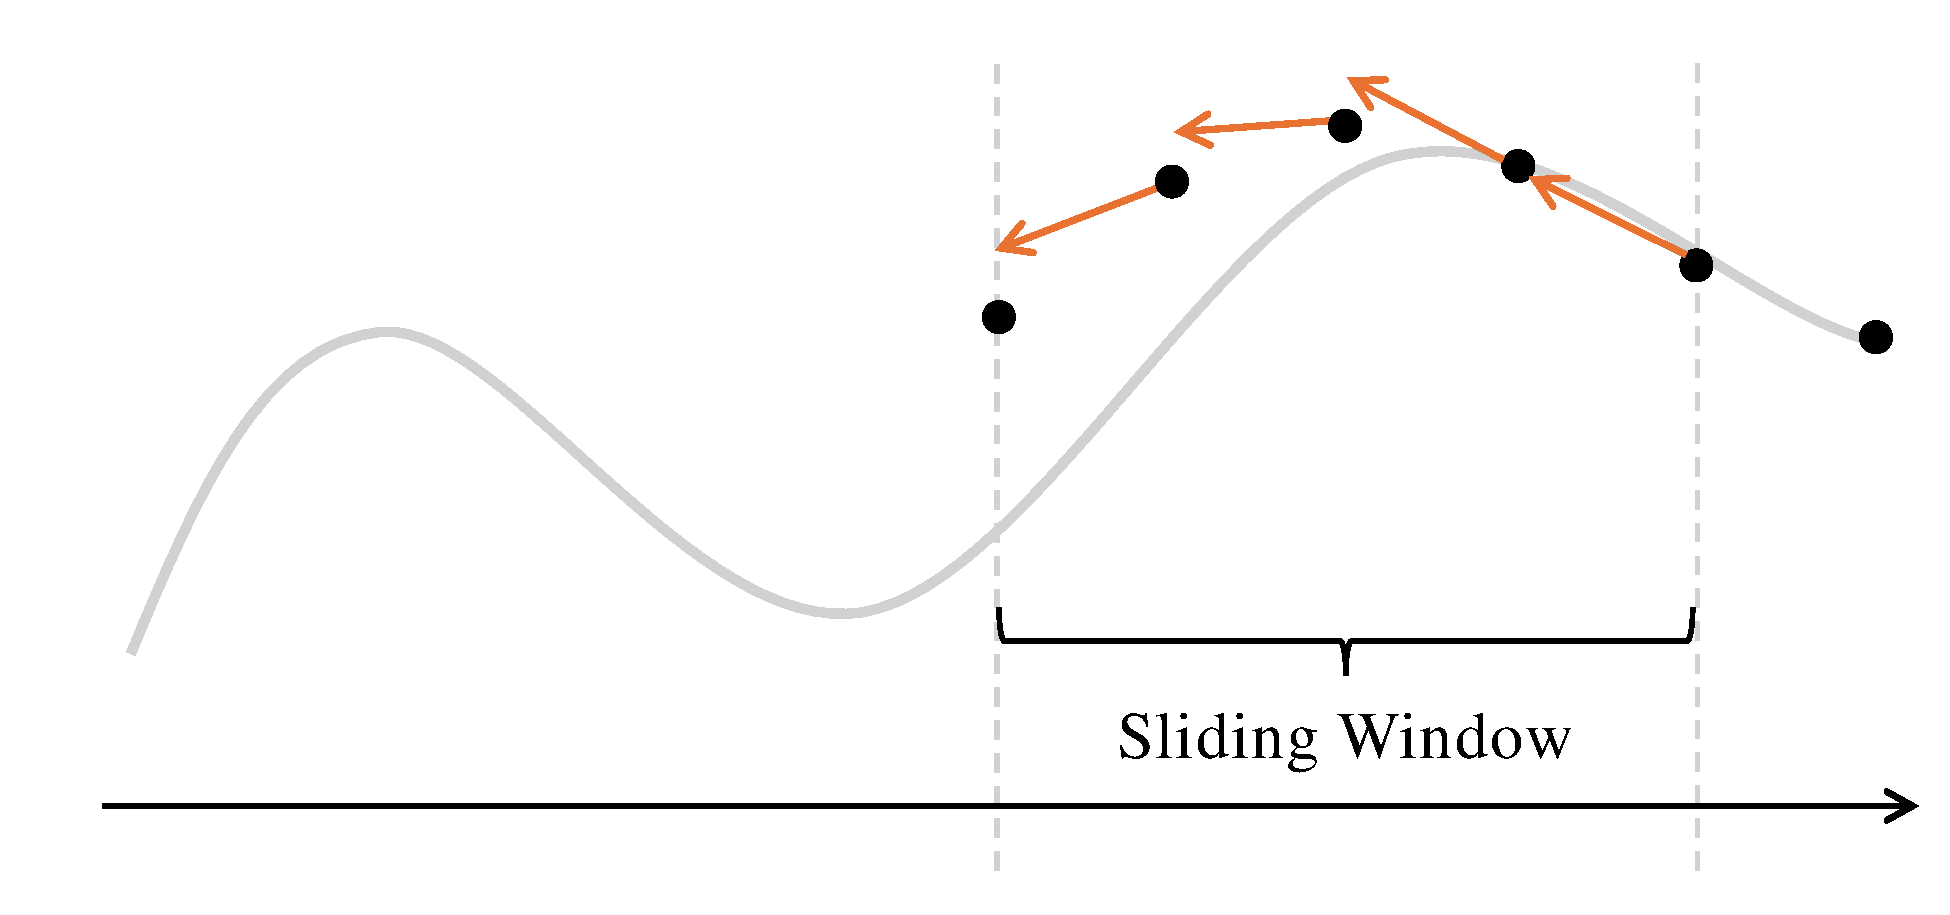
\includegraphics[width=\linewidth]{Images/PartC/paradigm-1.pdf}
        \caption{计算漂移 $\rvx^{(k)}_{\ell:\ell+p}$ 在大小的批处理窗口上 $p=4$，并联}
        \label{fig:picard_1}
    \end{minipage}
    \hspace{0.03\textwidth} 
    \begin{minipage}[t]{0.30\textwidth}
        \centering
        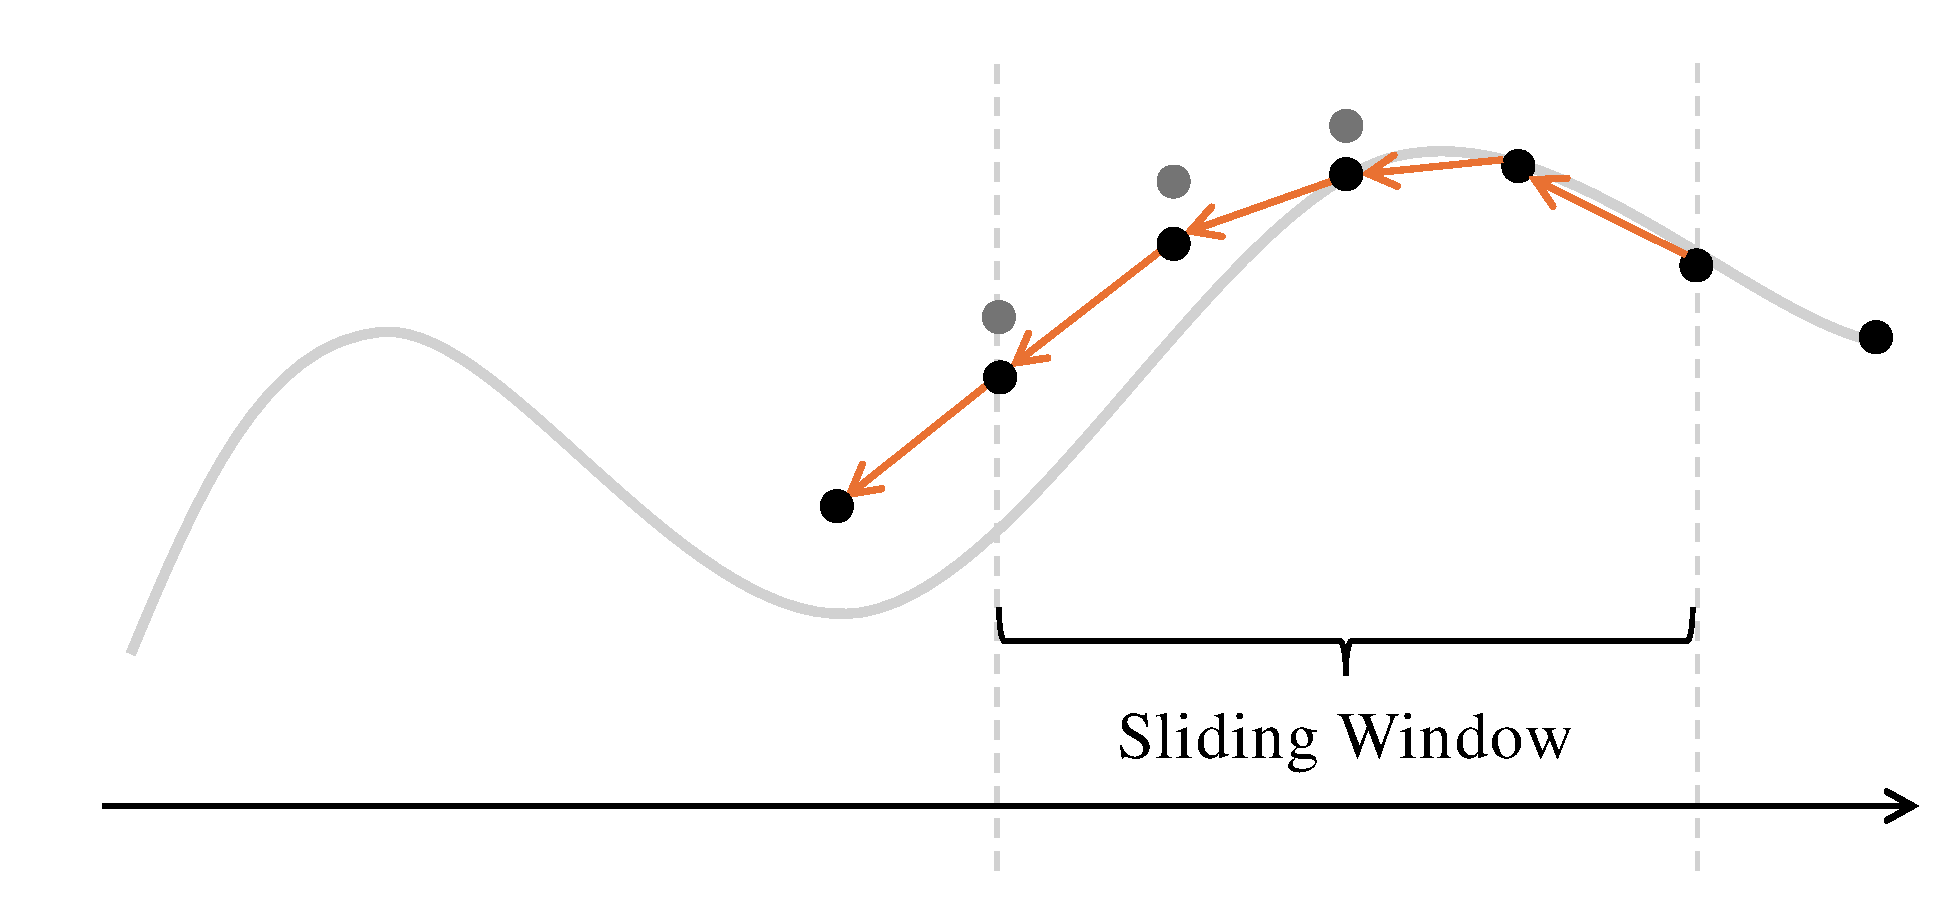
\includegraphics[width=\linewidth]{Images/PartC/paradigm-2.pdf}
        \caption{将值更新为 $\rvx^{(k+1)}_{\ell:\ell+p}$ 使用窗口中点的累积漂移}
        \label{fig:picard_2}
    \end{minipage}
    \hspace{0.03\textwidth} 
    \begin{minipage}[t]{0.30\textwidth}
        \centering
        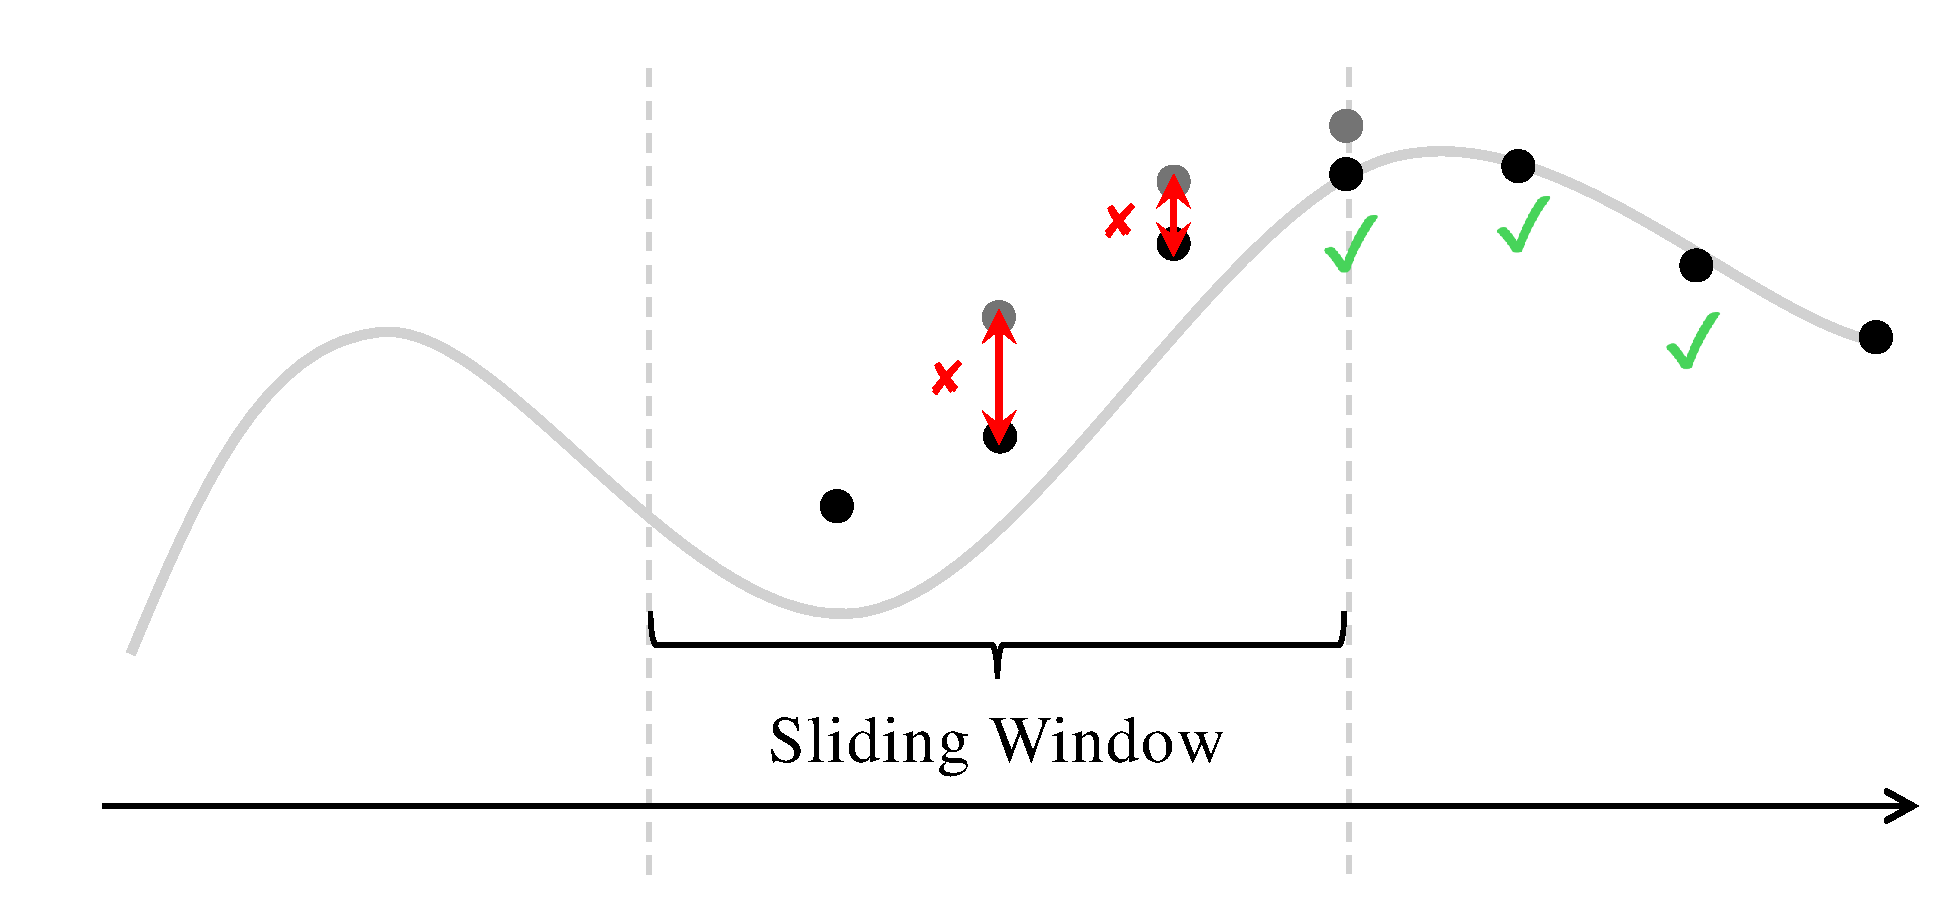
\includegraphics[width=\linewidth]{Images/PartC/paradigm-3.pdf}
        \caption{根据错误确定窗口向前滑动多远 $\lVert \rvx^{(k+1)}_i - \rvx^{(k)}_i \rVert^2$.}
        \label{fig:picard_3}
    \end{minipage}
    
    \figcredit{改编自 \citet{shih2023parallel}.}
    \label{fig:picard}
\end{figure}


离散 Picard 更新 \Cref{eq:discrete_picard_decreasing} 表示每个 $\rvx^{(k+1)}_j$ 作为固定初始值 $\rvx_T$ 减去漂移的累积和。为了限制内存并利用并行硬件，可以方便地将相同的想法局部应用到短的滑动索引块上。固定窗口长度 $p$ 和左索引 $\ell$;然后窗口覆盖
$j=\ell,\ldots,\ell+p$ 与 $t_\ell>t_{\ell+1}>\cdots>t_{\ell+p}$。迭代期间 $k$:

\subparagraph{步骤 1. 窗口上的并行漂移评估。}
并行计算并仅使用先前的迭代，
\[
\rvv_{\bphi^\times} \big(\rvx^{(k)}_{\ell+i}, t_{\ell+i}\big),
\quad i=0,1,\ldots,p-1.
\]
这些是 $p$ 从左边缘前进所需的局部增量
$t_\ell$ 窗外。\subparagraph{步骤 2. 左锚定累积更新。}
通过锚定在 $j=\ell$ 并累积子区间的漂移来形成窗口更新：
\begin{equation}\label{eq:window_update}
\rvx^{(k+1)}_{\ell+j+1}
 = 
\rvx^{(k)}_{\ell}
 - \Delta t \sum_{i=0}^{j}
\rvv_{\bphi^\times} \big(\rvx^{(k)}_{\ell+i}, t_{\ell+i}\big),
\quad j=0,1,\ldots,p-1.
\end{equation}
这是本地的、窗口化的对应项
\Cref{eq:discrete_picard_decreasing}，当前左边界值
$\rvx^{(k)}_\ell$ 用作窗口的锚点。减号
反映了时间递减的方向。内部和是前缀和
加窗漂移，因此可以有效地生成所有部分和
并行硬件。

\subparagraph{步骤 3. 进度控制和窗口前进。}
在当前窗口上形成左锚定累积更新（Step~2），
我们现在决定将该窗口滑动多远。我们测量局部收敛
通过逐点皮卡德变化
\[
\mathtt{error}_j
:=
\big\|\rvx^{(k+1)}_{\ell+j}-\rvx^{(k)}_{\ell+j}\big\|^2,
\quad j=1,\ldots,p-1,
\]
并将其与规定的公差 $\mathtt{tol}_{\ell+j}$ 进行比较。也就是说，$\mathtt{error}_j$ 测量节点 $\ell+j$ 的迭代在最后一次 Picard 期间发生了多少变化
更新。如果这个数字很小，则表明两者之间存在局部一致性
逐次逼近，从而实现定点的局部收敛
在该节点进行迭代。如果很大，说明该节点还没有稳定下来，需要
更多皮卡德平滑。


\emph{stride} 被选为窗口中失败的第一个索引
测试（如果没有失败，则使用全窗口长度 $p$）：
\[
\mathtt{stride}
:=
\min\Big(\,\{\,j\ge 1:\ \mathtt{error}_j>\mathtt{tol}_{\ell+j}\,\}\ \cup\ \{p\}\Big).
\]
然后我们通过设置$\ell \leftarrow \ell+\mathtt{stride}$来滑动窗口。  换句话说：我们接受从左边缘到（但不包括）的所有节点
第一个尚未收敛的；如果所有节点都收敛，我们接受
整个窗口。然后我们将窗口滑动到许多已接受的节点，
$\ell \leftarrow \ell+\mathtt{stride}$，然后继续。这提前了
最大窗口长度$p$，从不跳过任何未满足其要求的节点
宽容。如果滑动会超出网格末端 $M$，我们将窗口截断为
$p \leftarrow \min\{p,\,M-\ell\}$ 并继续。



当窗口向前移动时，它会发现新的时间节点
还没有值。要在那里开始 Picard 迭代，我们只需复制该值
从窗口的左边界开始，并将其用作初始猜测。这个
“不断外推”是便宜且稳定的，并且将被稍后纠正
更新。如果需要，可以用更准确的猜测来代替它，例如线性
或根据过去的点进行多项式外推。

至此，ParaDiGMS 的流程就完成了。我们总结了 \Cref{alg:paradigms} 中的算法。

\begin{algorithm}[t]
  \caption{带滑动窗口的 ParaDiGMS}
  \label{alg:paradigms}
  \begin{algorithmic}[1]
    \Require 漂移 $\rvv_{\bphi^\times}(\rvx,t)$; $\{t_j\}_{j=0}^{M}$;窗口长度 $p$; $\{\mathtt{tol}_j\}_{j=1}^{M}$
    \Ensure 近似轨迹 $\{\rvx^{(k)}_j\}_{j=0}^{M}$ 与 $\rvx^{(k)}_M$ 在 $t=0$
    \State $k \gets 0$, $\ell \gets 0$ 
    \State 样品 $\rvx^{(0)}_0 \sim p_{\mathrm{prior}}$;设置 $\rvx^{(0)}_j \gets \rvx^{(0)}_0$ 用于 $j=1,\ldots,\min(p,M)$  \Statex \Comment{常数外推}
    \While{$\ell < M$}
      \State $J \gets \min(p,  M-\ell)$   \Comment{当前窗口长度}
      \State \textbfs{第 1 步：并行} 
      \State 对于 $i=0,\ldots,J-1$: $g_i \gets \rvv_{\bphi^\times} \big(\rvx^{(k)}_{\ell+i},\, t_{\ell+i}\big)$ 
      \Statex \Comment{与先前迭代的偏差（皮卡德冻结）}
      \State 计算前缀和 $S_j \gets \sum_{i=0}^{j} g_i$ 用于 $j=0,\ldots,J-1$ 
      \Statex \Comment{扫描窗口漂移}
      \State \textbfs{步骤 2：累积更新} 
      \State 对于 $j=0,\ldots,J-1$: $\displaystyle \rvx^{(k+1)}_{\ell+j+1} \gets \rvx^{(k)}_{\ell} - \Delta t\, S_j$ 
      \Statex \Comment{左锚定更新；参见\ \Cref{eq:window_update}}
      \State \textbfs{步骤 3：进度控制和窗口前进} 
      \State 对于 $j=1,\ldots,J-1$: $\mathtt{error}_j \gets \big\|\rvx^{(k+1)}_{\ell+j}-\rvx^{(k)}_{\ell+j}\big\|^2$ \Statex \Comment{逐点皮卡德变化}
      \State $\displaystyle \mathtt{stride} \gets \min \Big(\,\{\,j\in\{1,\ldots,J-1\}:~\mathtt{error}_j>\mathtt{tol}_{\ell+j}\,\}\ \cup\ \{J\}\Big)$
      \State \textbfs{初始化新节点} 
        \State 对于 $r=1,\ldots,\min\{\mathtt{stride},\,M-\ell-J\}$:
        $\rvx^{(k+1)}_{\ell+J+r}
        \gets
        \rvx^{(k+1)}_{\ell+J}$ 
      \Statex \Comment{不断外推到新公开的指数}
      \State $\ell \gets \ell + \mathtt{stride}$;\quad $k \gets k+1$
    \EndWhile
    \State \Return $\{\rvx^{(k)}_j\}_{j=0}^{M}$
  \end{algorithmic}
\end{algorithm}




\subsection{与时间步进求解器的关系}

\paragraph{滑动窗口尺寸的选择。}
要了解窗口大小的作用，首先考虑最小的选择 $p=1$。在这种情况下，不存在时间并行性，并且该方法简化为其顺序基础更新。对于左端点离散化 \Cref{eq:window_update}，这只是一个简单的欧拉步骤。更一般地说，ParaDiGMS 指定了如何并行化不同时间点的计算，而每个步骤使用的数值更新可以单独选择。例如，Euler 更新可以替换为 DDIM 或 DPM-Solver，给出 ParaDDIM 或 ParaDPMSolver。增加 $p$ 然后将更多时间点暴露给并行计算，而不改变底层时间网格或总步数 $M$。皮卡德迭代反复修正这些状态，使其与所选的基本求解器保持一致，并由规定的局部容差控制收敛。

\paragraph{与高阶求解器（例如 DPM）的兼容性。}
Picard 框架决定了如何并行更新和评估不同时间点的状态，而用于近似每个步骤的数值规则可以单独选择。例如，而不是左端点规则
\Cref{eq:window_update}，我们可以使用梯形法则：
\begin{align*}
\rvx^{(k+1)}_{\ell+j+1}
=
\rvx^{(k)}_{\ell}
-\Delta t\Bigg[
\tfrac{1}{2}
\rvv_{\bphi^\times}
\big(\rvx^{(k)}_{\ell},t_{\ell}\big)
+
\sum_{i=1}^{j}
\rvv_{\bphi^\times}
\big(\rvx^{(k)}_{\ell+i},t_{\ell+i}\big)
+
\tfrac{1}{2}
\rvv_{\bphi^\times}
\big(\rvx^{(k)}_{\ell+j+1},t_{\ell+j+1}\big)
\Bigg],
\end{align*}
其中 $j=0,\ldots,p-1$。对于 $j=0$，这是熟悉的一步梯形更新，使用两个
端点漂移。对于较大的$j$，同样的规则累加梯形
跨过窗口的贡献。由于所有漂移都是使用
之前的皮卡德迭代，它们仍然可以并行计算，而
内部贡献可以通过前缀和来累积。

更一般地，ParaDiGMS 可以使用现有的顺序采样器，例如
DDIM 或 DPM-Solver 作为其基础离散化。在这种情况下，皮卡德
更新是根据相应的基求解器增量构造的，而不是
与上面的梯形公式相比。精确的形式取决于
选择的求解器，因为高阶方法可能使用中间阶段或
之前的模型评估。

对于基于给定顺序求解器的 ParaDiGMS 构造，精确
定点收敛恢复相应的顺序离散
轨迹。在有限停止容差的情况下，最终结果还包含
除了离散化之外的剩余定点迭代误差
基本求解器的误差。

\newpage
\section{结束语}\label{sec:ch9_cr}

本章遇到了最重要的实际限制之一
扩散模型：其缓慢的迭代采样过程。我们已经探索过
无需训练的方法，通过更好的设计来加速生成
经验 PF-ODE 的数值求解器：
\begin{enumerate}
    \item 我们从 DDIM 开始，一阶因子指数积分器
    更新，以分析方式保留已知的扩散时间表，同时
    保持神经预测固定。
    \item 然后我们研究了DEIS，它把这个想法扩展到了高阶
    通过重用过去的模型评估来推断如何进行多步更新
    神经预测发生变化。
    \item 最后，我们研究了 DPM-Solver 系列，它介绍了
    log-SNR 时间坐标并构造高阶更新
    步内模型评估。 DPM-Solver\texttt{++}进一步发展
    数据预测公式中的单步和多步变体。
\end{enumerate}

这些方法共同说明了一个共同原则：利用分析方法
已知的扩散结构并集中数值近似
学习模型预测。他们的预测和时间不同
参数化，以及是否从其中获得高阶信息
步骤内阶段或上一步历史记录。 ParaDiGMS 提供了补充
通过定点跨时间重新组织计算来确定方向
迭代和并行评估。这种求解器的开发可以减少
采样成本从数百或数千个模型评估减少到仅数十个
许多实用的设置。然而，这些免训练方法从根本上来说仍然是迭代的：它们
数值上近似连续的生成轨迹，即使部分
计算可以并行化。这就提出了一个自然的问题：
\emph{ 能否通过一步或者几步就实现高质量生成？}

本专着的最后一部分~D通过以下方式探讨了这个问题
基于训练的加速。在\Cref{ch:distillation}中，我们研究
基于蒸馏的方法，快速 \textit{student} 生成器学习
重现缓慢的预训练 \textit{teacher} 的行为。在
\Cref{ch:fast-scratch}，我们转向直接学习几步的方法
由 ODE 流从头开始定义的生成器。

这种从设计更好的数值求解器到直接学习
生成解图的快速逼近旨在结合质量
具有一步或几步生成速度的扩散模型。


\clearpage
\newpage